\documentclass[twoside]{book}

% Packages required by doxygen
\usepackage{fixltx2e}
\usepackage{calc}
\usepackage{doxygen}
\usepackage[export]{adjustbox} % also loads graphicx
\usepackage{graphicx}
\usepackage[utf8]{inputenc}
\usepackage{makeidx}
\usepackage{multicol}
\usepackage{multirow}
\PassOptionsToPackage{warn}{textcomp}
\usepackage{textcomp}
\usepackage[nointegrals]{wasysym}
\usepackage[table]{xcolor}

% Font selection
\usepackage[T1]{fontenc}
\usepackage[scaled=.90]{helvet}
\usepackage{courier}
\usepackage{amssymb}
\usepackage{sectsty}
\renewcommand{\familydefault}{\sfdefault}
\allsectionsfont{%
  \fontseries{bc}\selectfont%
  \color{darkgray}%
}
\renewcommand{\DoxyLabelFont}{%
  \fontseries{bc}\selectfont%
  \color{darkgray}%
}
\newcommand{\+}{\discretionary{\mbox{\scriptsize$\hookleftarrow$}}{}{}}

% Page & text layout
\usepackage{geometry}
\geometry{%
  letterpaper,%
  top=2.5cm,%
  bottom=2.5cm,%
  left=2.5cm,%
  right=2.5cm%
}
\tolerance=750
\hfuzz=15pt
\hbadness=750
\setlength{\emergencystretch}{15pt}
\setlength{\parindent}{0cm}
\setlength{\parskip}{3ex plus 2ex minus 2ex}
\makeatletter
\renewcommand{\paragraph}{%
  \@startsection{paragraph}{4}{0ex}{-1.0ex}{1.0ex}{%
    \normalfont\normalsize\bfseries\SS@parafont%
  }%
}
\renewcommand{\subparagraph}{%
  \@startsection{subparagraph}{5}{0ex}{-1.0ex}{1.0ex}{%
    \normalfont\normalsize\bfseries\SS@subparafont%
  }%
}
\makeatother

% Headers & footers
\usepackage{fancyhdr}
\pagestyle{fancyplain}
\fancyhead[LE]{\fancyplain{}{\bfseries\thepage}}
\fancyhead[CE]{\fancyplain{}{}}
\fancyhead[RE]{\fancyplain{}{\bfseries\leftmark}}
\fancyhead[LO]{\fancyplain{}{\bfseries\rightmark}}
\fancyhead[CO]{\fancyplain{}{}}
\fancyhead[RO]{\fancyplain{}{\bfseries\thepage}}
\fancyfoot[LE]{\fancyplain{}{}}
\fancyfoot[CE]{\fancyplain{}{}}
\fancyfoot[RE]{\fancyplain{}{\bfseries\scriptsize Generated by Doxygen }}
\fancyfoot[LO]{\fancyplain{}{\bfseries\scriptsize Generated by Doxygen }}
\fancyfoot[CO]{\fancyplain{}{}}
\fancyfoot[RO]{\fancyplain{}{}}
\renewcommand{\footrulewidth}{0.4pt}
\renewcommand{\chaptermark}[1]{%
  \markboth{#1}{}%
}
\renewcommand{\sectionmark}[1]{%
  \markright{\thesection\ #1}%
}

% Indices & bibliography
\usepackage{natbib}
\usepackage[titles]{tocloft}
\setcounter{tocdepth}{3}
\setcounter{secnumdepth}{5}
\makeindex

% Hyperlinks (required, but should be loaded last)
\usepackage{ifpdf}
\ifpdf
  \usepackage[pdftex,pagebackref=true]{hyperref}
\else
  \usepackage[ps2pdf,pagebackref=true]{hyperref}
\fi
\hypersetup{%
  colorlinks=true,%
  linkcolor=blue,%
  citecolor=blue,%
  unicode%
}

% Custom commands
\newcommand{\clearemptydoublepage}{%
  \newpage{\pagestyle{empty}\cleardoublepage}%
}

\usepackage{caption}
\captionsetup{labelsep=space,justification=centering,font={bf},singlelinecheck=off,skip=4pt,position=top}

%===== C O N T E N T S =====

\begin{document}

% Titlepage & ToC
\hypersetup{pageanchor=false,
             bookmarksnumbered=true,
             pdfencoding=unicode
            }
\pagenumbering{alph}
\begin{titlepage}
\vspace*{7cm}
\begin{center}%
{\Large C\+P\+P\+\_\+\+Birdtracker }\\
\vspace*{1cm}
{\large Generated by Doxygen 1.8.13}\\
\end{center}
\end{titlepage}
\clearemptydoublepage
\pagenumbering{roman}
\tableofcontents
\clearemptydoublepage
\pagenumbering{arabic}
\hypersetup{pageanchor=true}

%--- Begin generated contents ---
\chapter{R\+E\+A\+D\+ME}
\label{md_README}
\Hypertarget{md_README}


\section*{The Lun\+Aero Project}

Lun\+Aero is a hardware and software project using Open\+CV to automatically track birds as they migrate in front of the moon. This repository contains software used to track bird silhouettes from video produced by the Lun\+Aero moontracking robot. For information on the hardware and software for the robot, please see \href{https://github.com/BlueNalgene/LunAero_C}{\tt https\+://github.\+com/\+Blue\+Nalgene/\+Lun\+Aero\+\_\+C} .

Created by , working in the lab of -\/\+S-\/\+Bridge.

\section*{Birdtracker\+\_\+\+C\+PP vs. Lun\+Aero}

The Birdtracker\+\_\+\+C\+PP repository is an updated version of the Lun\+Aero silhouette tracking software. The previous implementation (archived at \href{https://github.com/BlueNalgene/LunAero}{\tt https\+://github.\+com/\+Blue\+Nalgene/\+Lun\+Aero}) was a Python 3 script. This updated version is C++ code designed for Linux, and includes many improvements, additional features, and is generally more mature code.

\subsection*{Software Install Instructions}

\subsubsection*{Option 1\+: Compile this Repository}

To follow my instructions, you need to use the Linux terminal, where you can copy and paste the following scripts. To open the Linux terminal, press {\ttfamily ctrl}+{\ttfamily alt}+{\ttfamily t}.

When you install this for the first time on to a Linux system, you will need certain repositories installed to make it. If you are using a Debian-\/like operating system (e.\+g. Ubuntu or Mate), use the following command in your terminal. (Note\+: this looks way more daunting than it really is, your OS will have most of these installed with a default configuration)\+:


\begin{DoxyCode}
sudo apt update
sudo apt -y install git libgcc-7-dev libc6 libstdc++-7-dev libc6-dev \(\backslash\)
libgl1 libqt5test5 libqt5opengl5 libqt5widgets5 libqt5gui5 libqt5core5a \(\backslash\)
libdc1394-22 libavcodec-extra57 libavformat57 libavutil55 libswscale4 \(\backslash\)
libpng16-16 libtiff5 libopenexr22 libtbb2 zlib1g libglx0 libglvnd0 \(\backslash\)
libharfbuzz0b libicu60 libdouble-conversion1 libglib2.0-0 libraw1394-11 \(\backslash\)
libusb-1.0-0 libswresample2 libwebp6 libcrystalhd3 libva2 libzvbi0 \(\backslash\)
libxvidcore4 libx265-146 libx264-152 libwebpmux3 libwavpack1 libvpx5 \(\backslash\)
libvorbisenc2 libvorbis0a libvo-amrwbenc0 libtwolame0 libtheora0 \(\backslash\)
libspeex1 libsnappy1v5 libshine3 librsvg2-2 libcairo2 libopus0 \(\backslash\)
libopenjp2-7 libopencore-amrwb0 libopencore-amrnb0 libmp3lame0 libgsm1 \(\backslash\)
liblzma5 libssh-gcrypt-4 libopenmpt0 libbluray2 libgnutls30 libxml2 \(\backslash\)
libgme0 libchromaprint1 libbz2-1.0 libx11-6 libdrm2 libvdpau1 \(\backslash\)
libva-x11-2 libva-drm2 libjbig0 libjpeg-turbo8 libilmbase12 libfreetype6 \(\backslash\)
libgraphite2-3 libpcre3 libudev1 libsoxr0 libnuma1 libogg0 \(\backslash\)
libgdk-pixbuf2.0-0 libpangocairo-1.0-0 libpangoft2-1.0-0 libpango-1.0-0 \(\backslash\)
libfontconfig1 libcroco3 libffi6 libpixman-1-0 libxcb-shm0 libxcb1 \(\backslash\)
libxcb-render0 libxrender1 libxext6 libgcrypt20 libgssapi-krb5-2 \(\backslash\)
libmpg123-0 libvorbisfile3 libp11-kit0 libidn2-0 libunistring2 \(\backslash\)
libtasn1-6 libnettle6 libhogweed4 libgmp10 libxfixes3 libgomp1 \(\backslash\)
libselinux1 libmount1 libthai0 libexpat1 libxau6 libxdmcp6 libgpg-error0 \(\backslash\)
libkrb5-3 libk5crypto3 libcom-err2 libkrb5support0 libblkid1 libdatrie1 \(\backslash\)
libbsd0 libkeyutils1 libuuid1
\end{DoxyCode}


Then comes the step that is actually daunting. This program requires Open\+CV compiled with {\ttfamily contrib}. This means you M\+U\+ST compile Open\+CV from source. This has been tested for Open\+CV version {\ttfamily 4.\+4.\+0-\/pre}. Older versions may not work. There are many options for compiling, I used the following on my Ubuntu box\+:


\begin{DoxyItemize}
\item Install prerequisites 
\begin{DoxyCode}
sudo apt install build-essential cmake git pkg-config libgtk-3-dev \(\backslash\)
libavcodec-dev libavformat-dev libswscale-dev libv4l-dev \(\backslash\)
libxvidcore-dev libx264-dev libjpeg-dev libpng-dev libtiff-dev \(\backslash\)
gfortran openexr libatlas-base-dev python3-dev python3-numpy \(\backslash\)
libtbb2 libtbb-dev libdc1394-22-dev
\end{DoxyCode}

\item Download files 
\begin{DoxyCode}
mkdir ~/opencv\_build && cd ~/opencv\_build
git clone https://github.com/opencv/opencv.git
git clone https://github.com/opencv/opencv\_contrib.git
\end{DoxyCode}

\item Prep make options 
\begin{DoxyCode}
cd ~/opencv\_build/opencv
mkdir build && cd build
cmake -D CMAKE\_BUILD\_TYPE=RELEASE \(\backslash\)
    -D CMAKE\_INSTALL\_PREFIX=/usr/local \(\backslash\)
    -D INSTALL\_C\_EXAMPLES=ON \(\backslash\)
    -D INSTALL\_PYTHON\_EXAMPLES=ON \(\backslash\)
    -D OPENCV\_GENERATE\_PKGCONFIG=ON \(\backslash\)
    -D OPENCV\_EXTRA\_MODULES\_PATH=~/opencv\_build/opencv\_contrib/modules \(\backslash\)
    -D BUILD\_EXAMPLES=ON ..
\end{DoxyCode}

\item Make the files using multiple threads and install. Get coffee during this step. 
\begin{DoxyCode}
make -j8
sudo make install
\end{DoxyCode}

\end{DoxyItemize}

Next, use {\ttfamily git} to pull this repository. Once the Lun\+Aero {\ttfamily git} repository is pulled, you can compile it. To do this, execute the lines in the terminal\+:


\begin{DoxyCode}
cd /home/$USER/Documents
git https://github.com/BlueNalgene/CPP\_Birdtracker.git
cd Birdtracker\_CPP
\end{DoxyCode}


This script downloads the everything you need to compile the program from this {\ttfamily git} repository. Once you have the repository on your Raspberry Pi and have installed all of the relevant packages from the {\ttfamily apt} command above, enter the Lun\+Aero\+\_\+C folder, and issue the following command\+:


\begin{DoxyCode}
make
\end{DoxyCode}


The {\ttfamily make} command follows the instructions from the {\ttfamily Makefile} to compile your program. If you ever make changes to the source material, remember to edit the {\ttfamily Makefile} to reflect changes to the packages used or the required C++ files. If {\ttfamily make} runs correctly, your terminal will print some text that looks like {\ttfamily g++ blah blah -\/o frame\+\_\+extractor.\+o} spanning a few lines. If the output is significantly longer than that and includes words like E\+R\+R\+OR or W\+A\+R\+N\+I\+NG, something may have gone wrong, and you should read the error messages to see if something needs to be fixed.

\subsubsection*{Option 2 (experimental)\+: Download a Pre-\/\+Compiled Binary Release}

\subsection*{Running Lun\+Aero}

To run the {\ttfamily frame\+\_\+extractor.\+o}, use the Linux terminal. There, you enter the command for the program and information about the video you want to run the program on. It is convenient if you navigate to the directory where you made the file\+:


\begin{DoxyCode}
/path/to/Birdtracker\_CPP
\end{DoxyCode}


\subsubsection*{Edit the Settings}

A file called {\ttfamily settings.\+cfg} has been provided to give the user the ability to modify settings without needing to recompile. Before running, Lun\+Aero for the first time, it is prudent to check that you are happy with the default settings. This is especially true for the General Settings at to top of the file.

A python3 script called {\ttfamily \hyperlink{fog__removal_8py}{fog\+\_\+removal.\+py}} has been added to simplify selecting the appropriate value for B\+L\+A\+C\+K\+O\+U\+T\+\_\+\+T\+H\+R\+E\+SH. Run this script prior to running a video to visually determine the appropriate value for this variable.

\subsubsection*{Command Options}

The following options are available for command line switches\+:

\tabulinesep=1mm
\begin{longtabu} spread 0pt [c]{*{4}{|X[-1]}|}
\hline
\rowcolor{\tableheadbgcolor}\textbf{ Full Command }&\textbf{ Short Command }&\textbf{ Expected Input }&\textbf{ Description  }\\\cline{1-4}
\endfirsthead
\hline
\endfoot
\hline
\rowcolor{\tableheadbgcolor}\textbf{ Full Command }&\textbf{ Short Command }&\textbf{ Expected Input }&\textbf{ Description  }\\\cline{1-4}
\endhead
{\ttfamily -\/-\/help} &{\ttfamily -\/h} &none &Show this info \\\cline{1-4}
{\ttfamily -\/-\/version} &{\ttfamily -\/v} &none &Print version info to terminal \\\cline{1-4}
{\ttfamily -\/-\/input} &{\ttfamily -\/i} &path to vid file&Specify path to input video \\\cline{1-4}
{\ttfamily -\/-\/config-\/file}&{\ttfamily -\/c} &path to config &Specify config file \\\cline{1-4}
{\ttfamily -\/-\/osf-\/path} &{\ttfamily -\/osf} &url to osf vid &Specify path to osf video \\\cline{1-4}
\end{longtabu}
The \char`\"{}\+Short Command\char`\"{} is just a helpful shorter version to replace the full command. Using either the {\ttfamily -\/-\/help} or {\ttfamily -\/-\/version} commands will print the relevant info to the terminal and exit, without running the full program. Each command or input must be separated by a space.

Each of the commands {\ttfamily -\/-\/input}, {\ttfamily -\/-\/config-\/file}, and {\ttfamily -\/-\/osf-\/path} require input arguments to follow the switch. These inputs are paths to the local storage location (in the case of {\ttfamily -\/-\/input} and {\ttfamily -\/-\/config-\/file}) or a url path (in the case of {\ttfamily -\/-\/osf-\/path}). If any of these switches are issued without an appropriate path argument following it, the program will crash. You may not issue both the {\ttfamily -\/-\/input} and {\ttfamily -\/-\/osf-\/path} in the same terminal command, as these switches conflict. (You can only have one source video!). You do not need to issue a {\ttfamily -\/-\/config-\/file} switch if you are using the {\ttfamily settings.\+cfg} file stored in the default location.

Some example commands\+:


\begin{DoxyCode}
./frame\_extractor.o -i /path/to/video.mp4
\end{DoxyCode}
 
\begin{DoxyCode}
./frame\_extractor.o -i "/path/to/video with spaces.mp4"
\end{DoxyCode}



\begin{DoxyCode}
./frame\_extractor.o -c /path/to/special\_config.cfg -osf osfstorage/path/to/video.mp4
\end{DoxyCode}


Remember\+: any time you want to check the usage information to view what each command switch does, use {\ttfamily -\/-\/help} in terminal, e.\+g.\+:


\begin{DoxyCode}
./frame\_extractor.o --help
\end{DoxyCode}


\subsubsection*{Using videos from O\+SF}

Run Birdtracker\+\_\+\+C\+PP on videos directly from storage repositories on Open Science Framework (O\+SF), you need to do some extra steps to pull in the A\+PI and enable access.


\begin{DoxyItemize}
\item The Python package {\ttfamily O\+S\+F\+Client} must be installed on your system. To install it, use the {\ttfamily pip} package manager e.\+g.\+: 
\begin{DoxyCode}
pip3 install OSFClient --user
\end{DoxyCode}

\item You must configure O\+S\+F\+Client on your system if you are using a password protected repository. To do this, add an environmental variable to your terminal for the entry \char`\"{}\+O\+S\+F\+\_\+\+P\+A\+S\+S\+W\+O\+R\+D\char`\"{}. On my system, this is easiest by editing the {\ttfamily .bashrc} file to contain the export command. 
\begin{DoxyCode}
nano /home/$USER/.bashrc
\end{DoxyCode}
 scroll to the bottom and add a line 
\begin{DoxyCode}
export OSF\_PASSWORD=[your password goes here]
\end{DoxyCode}
 This is the safest way to access according to the O\+S\+F\+Client maintainers, and I did not write this part of the code. Your milage may vary. If you are using a shared computer, be sure to remove your password when you are done.
\item You need to know the path to your file including the O\+SF repo ID and the storage name. The repository ID is a 5-\/digit alphanumeric code you can see when you got to the browser version of the site (osf.\+io/12345). This value must be written to the string {\ttfamily O\+S\+F\+P\+R\+O\+J\+E\+CT} in settings.\+cfg.
\item If you are using the defult O\+SF storage servers, you need to include the text \char`\"{}osfstorage\char`\"{} at the beginning of your path in the terminal. If you are using another storage server, please let me know what you have to use!
\end{DoxyItemize}

\subsubsection*{Valid Input File Formats}

The best choice for file format is M\+P4, as that is what everything is configured in the code to use. Other formats, such as the raw H264 video format which is output by Lun\+Aero, are converted to M\+P4 prior to starting the run. This video conversion may add time to your run, so consider this if you run this on shared systems with restricted time access.

Video conversion is done using {\ttfamily ffmpeg}, and this program is thus a prerequisite for use. If you are on a Linux system, you probably have {\ttfamily ffmpeg} installed already though. So don\textquotesingle{}t sweat it.

\subsection*{Behind the Curtain\+: What C\+P\+P\+\_\+\+Birdtracker does}

This program executes birdtracking efficiently by splitting tasks between C\+PU threads using the {\ttfamily fork()} command. Data which are shared between the forks such as frame numbers and matrices, is shared using memory mapping such that they can be accessed easily using pointers. The {\ttfamily wait} command is used to sync across forks, and the script executes code concurrently. When all frames of the video are completed, the data are passed through post-\/processing and the program exits. A simplified flowchart explains the process visually\+:


\begin{DoxyCode}
                    /-------\(\backslash\)
                    | start |
                    \(\backslash\)-------/
                        |
                   +---------+
                   | startup |
                   +---------+
                        |
                 +-------------+
                 | pre-process |
                 +-------------+
                        |
                   +--------+
                   | fork() |
                   +--------+
                        |
           +------------+
           |            |
       +-------+    +------+
       | fetch |  ->| sync | <------------------------\(\backslash\)
   +-->| next  |  | +------+                           \(\backslash\)
   |   | frame |  |     |                               \(\backslash\)
   |   +-------+  | +--------+                           \(\backslash\)
   |       |      | | fork() |                            \(\backslash\)
   |   +-------+  | +--------+                             \(\backslash\)
   |   | cycle |  |         |                               \(\backslash\)
   |   | frame |  |         +------------------------+       \(\backslash\)
   |   | buffer|  |         |                        |        \(\backslash\)
   |   +-------+  |         |                   +--------+    |
   |       |      |    +--------+               | cycle  |    |
   |   +-------+ /     | Tier 1 |               | frame  |    |
   |   |  wait |/      +--------+               | buf 2  |    |
   |   +-------+            |                   +--------+    |
   |       |           +--------+                    |        |
   |       ^           | Tier 2 |               +--------+    |
no |      / \(\backslash\)          +--------+               | Tier 3 |    |
   |     /   \(\backslash\)              |                   +--------+    |
   |    /     \(\backslash\)         +-------+                    |        |while
   |\_\_\_/ video \(\backslash\)        | wait/ |               +--------+    |loop
       \(\backslash\) done? /        |  sync |               | Tier 4 |    |
        \(\backslash\)     /         +-------+               +--------+    |
         \(\backslash\)   /              |                        |        |
          \(\backslash\) /               \(\backslash\)                    +-------+    |
           v                 \(\backslash\)                   | wait/ |    |
       yes |                  \(\backslash\)                  |  sync |    |
           |                   \(\backslash\)                 +-------+    |
   +--------------+             \(\backslash\)                 |           /
   | post-process |              \(\backslash\)                /          /
   +--------------+               \(\backslash\)              /          /
           |                       \(\backslash\)            /          /
           |                        \(\backslash\)          /          /
           |                         \(\backslash\)        /          /
           |                          \(\backslash\)      /          /
           |                          +------+         /
           |                          | kill |--------/
           |                          | fork |
           |                          +------+
        /-----\(\backslash\)
        | end |
        \(\backslash\)-----/
\end{DoxyCode}


Individual steps with more detail, but still simplified\+:


\begin{DoxyItemize}
\item startup\+:
\begin{DoxyItemize}
\item Parses the input commands
\item Redefines globals based on values from settings.\+cfg
\item Creates directories/empty data files
\item Instance and assign initial values to simple memory mapped regions
\end{DoxyItemize}
\item pre-\/process
\begin{DoxyItemize}
\item Load the video
\item Find the first frame where the moon is not touching the edge of the screen
\item Record initial values
\item Instance and assign initial values to complext memory mapped regions (frame buffers)
\item Prepare for fork()
\end{DoxyItemize}
\item F\+O\+RK T\+W\+I\+CE (three concurrent threads)
\begin{DoxyItemize}
\item fork0
\begin{DoxyItemize}
\item Check for exit command and sync status
\item Coordinate sync values across forks
\item Fetch the next frame
\item Prep frame (color conversion and cropping)
\item Store frame to the first buffer
\item Wait for sync.
\end{DoxyItemize}
\item fork1
\begin{DoxyItemize}
\item Check for exit command and sync status
\item Run Tier 1 and Tier 2 calculations
\item Wait for sync
\end{DoxyItemize}
\item fork2
\begin{DoxyItemize}
\item Check for exit command and sync status
\item Cycle first frame buffer with second frame buffer such that we have frame n and n-\/1 stored in the memory.
\item Run Tier 3 and Tier 4 calculations (requires n and n-\/1 frames)
\item Wait for sync
\end{DoxyItemize}
\end{DoxyItemize}
\item Kill unused fork and continue loop
\item If at end of the frames, kill all forks.
\item post-\/process
\begin{DoxyItemize}
\item Create slideshow
\item Concat data
\item Crop slideshow
\end{DoxyItemize}
\item Cleanup and Exit
\end{DoxyItemize}

\subsubsection*{Image Processing}

While there are a few image processing functions peppered through the code, most of these are simple color conversions and cropping. The meat of the image processing occurs within the \char`\"{}\+Tiers\char`\"{}. This is where contours of silhouettes crossing the moon are detected. They all operate on the same frames, but some \char`\"{}\+Tiers\char`\"{} offer different capabilities. Each have strengths and weaknesses.


\begin{DoxyItemize}
\item Tier 1\+: Strict adaptive threshold. In perfect conditions, this finds the majority of the large silhouettes. As the video becomes less perfect, the regime breaks down.
\item Tier 2\+: Loose adaptive threshold. In perfect conditions, this finds most of the smaller silhouettes which may be missed by Tier 1. However, it produces much more noise. As the video becomes less perfect, the regime breaks down.
\item Tier 3\+: Isotropic Laplacian filter. This is a very noisy filter which compares differences in the Laplacian across two frames. The result is blurred prior to detection, but much of the noise remains.
\item Tier 4\+: Un\+Canny filter. This experimental filter attempts to perform the steps used in the classic Canny filter backwards...across two frames. The Sobel and power steps of the Canny filter occur on each frame (n and n-\/1), then are added, rooted, and blurred. The result is passed through an edge thinner and the silhouettes are detected.
\end{DoxyItemize}

See the descriptions and code in the documentation \href{https://bluenalgene.github.io/CPP_Birdtracker/html/frame__extraction_8cpp.html}{\tt here}.

Each Tier process has values which may be manipulated in {\ttfamily settings.\+cfg} to customize the behavior during runtime.

\subsubsection*{Estimating Run Time}

On the test computer (Intel(\+R) Core(\+T\+M) i7-\/7500U C\+PU @ 2.\+70\+G\+Hz), the run time of this program is approximately 7 times the length of the input video, when the video is 1920x1080 at 30fps. So a 5 minute video will run in about 35 minutes.

Why does it take so long? Most of the computation time is spent opening and closing image files. This cannot be avoided.

\subsection*{The Output}

This program outputs several files during the run. The files are stored by default in the folder {\ttfamily Birdtracker\+\_\+\+Output}. Data files are stored in the {\ttfamily data} directory, if the settings are configured to output the frames, a {\ttfamily frames} directory is created containing {\ttfamily png} images of each frame in the video, this will also create an {\ttfamily output.\+mp4} slideshow of the frames.

\subsubsection*{The Data}

The data files in the {\ttfamily data} directory are as follows\+:

\tabulinesep=1mm
\begin{longtabu} spread 0pt [c]{*{2}{|X[-1]}|}
\hline
\rowcolor{\tableheadbgcolor}\textbf{ Filename }&\textbf{ Description  }\\\cline{1-2}
\endfirsthead
\hline
\endfoot
\hline
\rowcolor{\tableheadbgcolor}\textbf{ Filename }&\textbf{ Description  }\\\cline{1-2}
\endhead
log.\+log &Debugging log of run \\\cline{1-2}
metadata.\+csv &Input video metadata \\\cline{1-2}
boxes.\+csv &Boundary values of largest contour in frame \\\cline{1-2}
ellipses.\+csv &Properties of the largest contour in frame \\\cline{1-2}
Tier1.\+csv &Tier 1 detected silhouettes \\\cline{1-2}
Tier2.\+csv &Tier 2 detected silhouettes \\\cline{1-2}
Tier3.\+csv &Tier 3 detected silhouettes \\\cline{1-2}
Tier4.\+csv &Tier 4 detected silhouettes \\\cline{1-2}
mixed\+\_\+tiers.\+csv &All tier data mixed into a single file \\\cline{1-2}
offscreen\+\_\+moon.\+csv &Number of pixels where the moon is touching the screen edge \\\cline{1-2}
\end{longtabu}

\begin{DoxyItemize}
\item log.\+log -\/ If the boolean toggle {\ttfamily D\+E\+B\+U\+G\+\_\+\+C\+O\+UT} is set to {\ttfamily true} in settings.\+cfg, this log file will be created. Debugging messages are written to this file over the course of the run. Note, that this does not include any S\+T\+D\+O\+UT or S\+T\+D\+E\+RR messages. If there is an error message written to the terminal, for example, you must fetch that another way.
\item metadata.\+csv -\/ This file lists properties of the input video. Currently, that just includes the path to the input video.
\item boxes.\+csv -\/ This comma separated values (csv) file is mostly used for internal calculations. It is retained for diagnostic conveneince. The contents are values calculated which describe the location and size of the boundary points of the largest contour on each frame (presumably, this is the moon).
\item ellipses.\+csv -\/ This csv file lists properties of the largest contour on the screen more relevant to lunar calculations. Includes information such as the major and minor axis of the contour, area, and edges which touch the side of the screen.
\item Tier1.\+csv -\/ This csv lists all of the silhouettes detected using the stricter version of the {\ttfamily adaptive\+Threshold} method. See \href{https://bluenalgene.github.io/CPP_Birdtracker/html/frame__extraction_8cpp.html#a4f9b7b156d48ad3f147ff2b4edc01509}{\tt tier\+\_\+one()}
\item Tier2.\+csv -\/ This csv lists all of the silhouettes detected using the more lenient version of the {\ttfamily adaptive\+Threshold} method.
\item Tier3.\+csv -\/ This csv lists all of the silhouettes detected using isotropic Laplacian matching between frames.
\item Tier4.\+csv -\/ This csv lists all of the silhouettes detected using a new filter we are calling \char`\"{}\+Un\+Canny\char`\"{}, which is a reverse operation of the Canny filter between two frames.
\item mixed\+\_\+tiers.\+csv -\/ This csv is a convenience file which inclues everything from Tier$\ast$.csv in frame order. An additional column indicates which Tier method the line was generated from. Only created if {\ttfamily C\+O\+N\+C\+A\+T\+\_\+\+T\+I\+E\+RS} is set to {\ttfamily true}.
\item offscreen\+\_\+moon.\+csv -\/ This csv is a convenience file which edits down ellipses.\+csv to only report frames with non-\/zero values in one or more of the screen edge columns. Only created if {\ttfamily S\+I\+M\+P\+\_\+\+E\+LL} is set to {\ttfamily true}.
\end{DoxyItemize}

\subsubsection*{The Video}

If the {\ttfamily O\+U\+T\+P\+U\+T\+\_\+\+F\+R\+A\+M\+ES} value in settings is set to {\ttfamily true}, the Birdtracker will output every cropped frame to the {\ttfamily frames} directory as a {\ttfamily png} file with the naming format based on the frame number. These frames will remain in the directory unless the setting {\ttfamily E\+M\+P\+T\+Y\+\_\+\+F\+R\+A\+M\+ES} is set to {\ttfamily true}.

If the program is outputting frames, and {\ttfamily G\+E\+N\+\_\+\+S\+L\+I\+D\+E\+S\+H\+OW} is set to {\ttfamily true}, the frames will be contatenated into a slideshow saved as {\ttfamily output.\+mp4}.

If the program generates a slideshow, and {\ttfamily T\+I\+G\+H\+T\+\_\+\+C\+R\+OP} is set to {\ttfamily true}, the output video will be modified at the end of the run to crop each frame to a smaller size. The size of these frames is based on the extreme edges of the moon as reported in {\ttfamily boxes.\+csv} + 10 pixels. The cropped video is saved as {\ttfamily output.\+mp4}.

\subsection*{When Something Goes Wrong}

Something always goes wrong. It is the way of things. When something inevitably does go wrong with Lun\+Aero program, you should first check the logs. If the setting {\ttfamily D\+E\+B\+U\+G\+\_\+\+C\+O\+UT} in {\ttfamily settings.\+cfg} is set to {\ttfamily true} the program will attempt to save a log file in the same directory where the videos are saved for each run. This is very detailed, so searching for keywords like {\ttfamily W\+A\+R\+N\+I\+NG} and {\ttfamily E\+R\+R\+OR} are suggested.

\subsubsection*{Something Went Wrong...and it isn\textquotesingle{}t listed here}

If you need help, raise an Issue on this {\ttfamily git} repository with descriptive information so the package maintainer can help you.

\subsection*{What if I Want to Play with the Source Code?}

The source code is documented with the {\ttfamily Doxygen} standard. Every function and most variables are heavily commented to make it easy for you. You can view the documentation online by going to\+: \href{https://bluenalgene.github.io/CPP_Birdtracker/html/index.html}{\tt https\+://bluenalgene.\+github.\+io/\+C\+P\+P\+\_\+\+Birdtracker/html/index.\+html} . 
\chapter{File Index}
\section{File List}
Here is a list of all files with brief descriptions\+:\begin{DoxyCompactList}
\item\contentsline{section}{\hyperlink{fog__removal_8py}{fog\+\_\+removal.\+py} \\*A script to remove \char`\"{}fog\char`\"{} from around the moon prior to run }{\pageref{fog__removal_8py}}{}
\item\contentsline{section}{\hyperlink{frame__extraction_8cpp}{frame\+\_\+extraction.\+cpp} }{\pageref{frame__extraction_8cpp}}{}
\item\contentsline{section}{\hyperlink{frame__extraction_8hpp}{frame\+\_\+extraction.\+hpp} }{\pageref{frame__extraction_8hpp}}{}
\end{DoxyCompactList}

\chapter{File Documentation}
\hypertarget{frame__extraction_8cpp}{}\section{frame\+\_\+extraction.\+cpp File Reference}
\label{frame__extraction_8cpp}\index{frame\+\_\+extraction.\+cpp@{frame\+\_\+extraction.\+cpp}}
{\ttfamily \#include \char`\"{}frame\+\_\+extraction.\+hpp\char`\"{}}\newline
Include dependency graph for frame\+\_\+extraction.\+cpp\+:\nopagebreak
\begin{figure}[H]
\begin{center}
\leavevmode
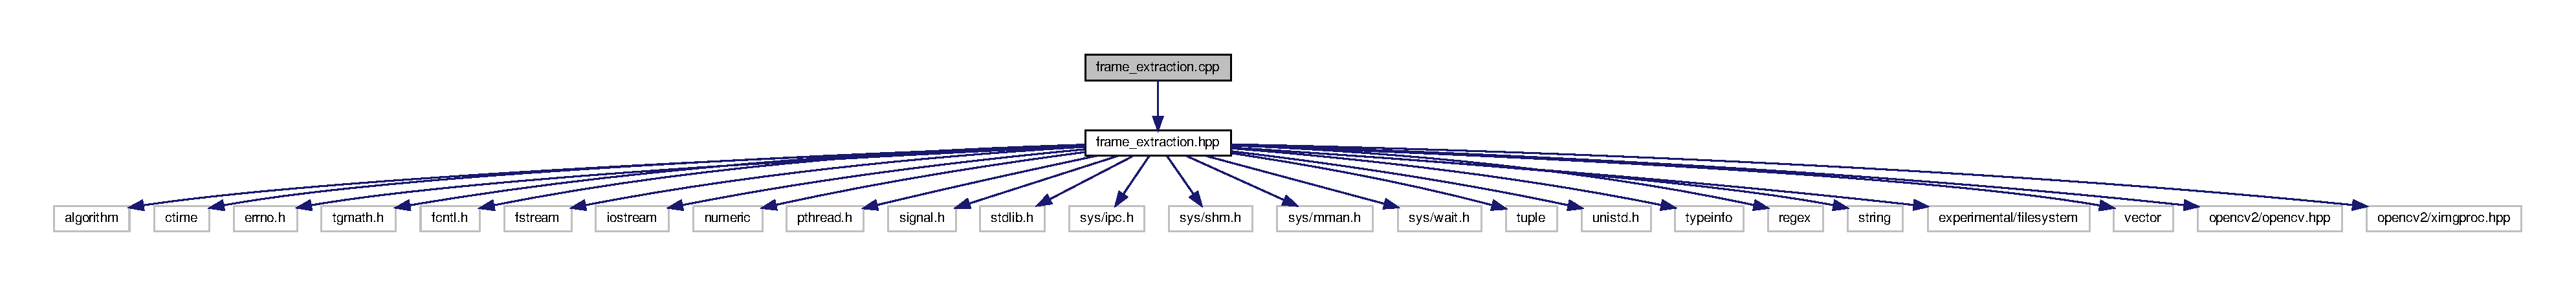
\includegraphics[width=350pt]{frame__extraction_8cpp__incl}
\end{center}
\end{figure}
\subsection*{Functions}
\begin{DoxyCompactItemize}
\item 
static Mat \hyperlink{frame__extraction_8cpp_afae27f2c8807b9a09243b93d512b504c}{shift\+\_\+frame} (Mat in\+\_\+frame, int shiftx, int shifty)
\item 
static Mat \hyperlink{frame__extraction_8cpp_a19b6b938855c1060791509f406645605}{corner\+\_\+matching} (Mat in\+\_\+frame, vector$<$ Point $>$ contour, int plusx, int plusy)
\item 
static vector$<$ int $>$ \hyperlink{frame__extraction_8cpp_a5ef2b91877d44dada29b478b53744af6}{test\+\_\+edges} (Mat in\+\_\+frame, vector$<$ Point $>$ contour, int te\+\_\+ret)
\item 
static int \hyperlink{frame__extraction_8cpp_a8b5c97016e3cad4475344f33f288bed4}{min\+\_\+square\+\_\+dim} (Mat in\+\_\+frame)
\item 
static vector$<$ int $>$ \hyperlink{frame__extraction_8cpp_a3ac94b4b4ad476fbcdd1ac7bc26b1fe1}{edge\+\_\+width} (vector$<$ Point $>$ contour)
\item 
static vector$<$ int $>$ \hyperlink{frame__extraction_8cpp_a3eefea9d7b7944b3c17145bf1f42ca1f}{edge\+\_\+height} (vector$<$ Point $>$ contour)
\item 
static int \hyperlink{frame__extraction_8cpp_a6ebd493f01eb54e528da257db0a75e99}{initial\+\_\+crop} (Mat in\+\_\+frame, int framecnt)
\item 
static int \hyperlink{frame__extraction_8cpp_a032ee30a958a27cdb3d5b419953ab584}{touching\+\_\+edges} (Mat in\+\_\+frame, vector$<$ Point $>$ contour)
\item 
static Mat \hyperlink{frame__extraction_8cpp_a8f336c75968d8ab7d3aa3c5c8ff74dbb}{traditional\+\_\+centering} (Mat in\+\_\+frame, vector$<$ vector$<$ Point $>$$>$ contours, int largest, Rect box)
\item 
static int \hyperlink{frame__extraction_8cpp_a2dab519501e6a1106a8b0b2cbfd52511}{first\+\_\+frame} (Mat in\+\_\+frame, int framecnt)
\item 
static int \hyperlink{frame__extraction_8cpp_a9c4e877be5c7a5b6c78cf2e81c09759f}{halo\+\_\+noise\+\_\+and\+\_\+center} (Mat in\+\_\+frame, int framecnt)
\item 
void \hyperlink{frame__extraction_8cpp_a89a8322bea357674e81ba9cbdefe0378}{signal\+\_\+callback\+\_\+handler} (int signum)
\item 
static Mat \hyperlink{frame__extraction_8cpp_adb0537fa8d7c5a8932f1abc66ee3d3f3}{apply\+\_\+dynamic\+\_\+mask} (Mat in\+\_\+frame, vector$<$ Point $>$ contour, int maskwidth)
\item 
static int \hyperlink{frame__extraction_8cpp_abc90f05608032b4730869812a513267f}{largest\+\_\+contour} (vector$<$ vector$<$ Point $>$$>$ contours)
\item 
static vector$<$ vector$<$ Point $>$ $>$ \hyperlink{frame__extraction_8cpp_a5a1b727e663ec81191fd584338c88227}{contours\+\_\+only} (Mat in\+\_\+frame)
\item 
static int \hyperlink{frame__extraction_8cpp_ab82da2f54d3288500af385f722ee691e}{box\+\_\+finder} (Mat in\+\_\+frame, bool do\+\_\+thresh)
\item 
static int \hyperlink{frame__extraction_8cpp_a3fe52ab2a13802c64a500f3b3fac618c}{box\+\_\+data} (Rect box, int framecnt)
\item 
static int \hyperlink{frame__extraction_8cpp_a5c53b5dffc43d3917a312ade756e53ee}{show\+\_\+usage} (string name)
\item 
static vector$<$ Point $>$ \hyperlink{frame__extraction_8cpp_a7564e59e35a0ba92812018e6ff847141}{qhe\+\_\+bigone} (Mat in\+\_\+frame)
\item 
static vector$<$ vector$<$ Point $>$ $>$ \hyperlink{frame__extraction_8cpp_ae9d9ad905beac19a35c93ee874a2c84c}{quiet\+\_\+halo\+\_\+elim} (vector$<$ vector$<$ Point $>$$>$ contours, vector$<$ Point $>$ bigone)
\item 
int \hyperlink{frame__extraction_8cpp_a26d746fc8b9f07ddace0bc9eef68c1c1}{tier\+\_\+one} (int framecnt, Mat in\+\_\+frame, vector$<$ Point $>$ bigone)
\item 
int \hyperlink{frame__extraction_8cpp_ad1e0683d8ff18ab579fbb2fcce6da1cc}{tier\+\_\+two} (int framecnt, Mat in\+\_\+frame, vector$<$ Point $>$ bigone)
\item 
int \hyperlink{frame__extraction_8cpp_a001a4318d62e5fcdb8b910d1f4dbab36}{tier\+\_\+three} (int framecnt, Mat in\+\_\+frame, Mat old\+\_\+frame, vector$<$ Point $>$ bigone)
\item 
int \hyperlink{frame__extraction_8cpp_abf1a9d948afc821690ec8c5c13dcee07}{tier\+\_\+four} (int framecnt, Mat in\+\_\+frame, Mat old\+\_\+frame, vector$<$ Point $>$ bigone)
\item 
int \hyperlink{frame__extraction_8cpp_aaee2ca25c5f0d375d48ec5b88dd6c1b3}{parse\+\_\+checklist} (std\+::string name, std\+::string value)
\item 
static std\+::string \hyperlink{frame__extraction_8cpp_ae5b18af36c3bf024f8a2dc5c4fe4242b}{out\+\_\+frame\+\_\+gen} (int framecnt)
\item 
std\+::string \hyperlink{frame__extraction_8cpp_a6aa2b943656a2bdc7bbb9a4f9e1adcd1}{space\+\_\+space} (std\+::string instring)
\item 
static int \hyperlink{frame__extraction_8cpp_a7e01b11733281d89519fef4c5abf705c}{edit\+\_\+contours\+\_\+for\+\_\+crop} ()
\item 
static int \hyperlink{frame__extraction_8cpp_ae3cfeeb43523e31ac7eebd51dbf58f9c}{get\+\_\+max\+\_\+ellipse\+\_\+params} ()
\item 
static int \hyperlink{frame__extraction_8cpp_a272c8275ab7a0918c5e6c9acf9afda50}{generate\+\_\+slideshow} ()
\item 
static int \hyperlink{frame__extraction_8cpp_a579a6e5cf9846789c07a88e72ef4a7a7}{concat\+\_\+tiers} ()
\item 
static int \hyperlink{frame__extraction_8cpp_aaf7c365254fb30ce3015aded4fdf1c9d}{off\+\_\+screen\+\_\+ellipse} ()
\item 
static int \hyperlink{frame__extraction_8cpp_a34a2b5ae307c281071a717fc2d1fb0c6}{post\+\_\+processing} ()
\item 
std\+::string \hyperlink{frame__extraction_8cpp_a0053c162fe33c7a2536d9b87dc7f3260}{tail} (std\+::string const \&source, size\+\_\+t const length)
\item 
int \hyperlink{frame__extraction_8cpp_a0ddf1224851353fc92bfbff6f499fa97}{main} (int argc, char $\ast$argv\mbox{[}$\,$\mbox{]})
\end{DoxyCompactItemize}


\subsection{Function Documentation}
\mbox{\Hypertarget{frame__extraction_8cpp_adb0537fa8d7c5a8932f1abc66ee3d3f3}\label{frame__extraction_8cpp_adb0537fa8d7c5a8932f1abc66ee3d3f3}} 
\index{frame\+\_\+extraction.\+cpp@{frame\+\_\+extraction.\+cpp}!apply\+\_\+dynamic\+\_\+mask@{apply\+\_\+dynamic\+\_\+mask}}
\index{apply\+\_\+dynamic\+\_\+mask@{apply\+\_\+dynamic\+\_\+mask}!frame\+\_\+extraction.\+cpp@{frame\+\_\+extraction.\+cpp}}
\subsubsection{\texorpdfstring{apply\+\_\+dynamic\+\_\+mask()}{apply\_dynamic\_mask()}}
{\footnotesize\ttfamily static Mat apply\+\_\+dynamic\+\_\+mask (\begin{DoxyParamCaption}\item[{Mat}]{in\+\_\+frame,  }\item[{vector$<$ Point $>$}]{contour,  }\item[{int}]{maskwidth }\end{DoxyParamCaption})\hspace{0.3cm}{\ttfamily [static]}}

This function masks out the edges of the input frame based on the contour. The maskwidth determines how much to mask out.


\begin{DoxyParams}{Parameters}
{\em in\+\_\+frame} & Open\+CV matrix image, 16-\/bit single depth format \\
\hline
{\em contour} & Open\+CV Point vectors of int-\/int point contour edges. Use the output from \char`\"{}bigone\char`\"{} here. \\
\hline
{\em maskwidth} & \\
\hline
\end{DoxyParams}
\begin{DoxyReturn}{Returns}
in\+\_\+frame The modified in\+\_\+frame from the input params 
\end{DoxyReturn}
Here is the caller graph for this function\+:\nopagebreak
\begin{figure}[H]
\begin{center}
\leavevmode
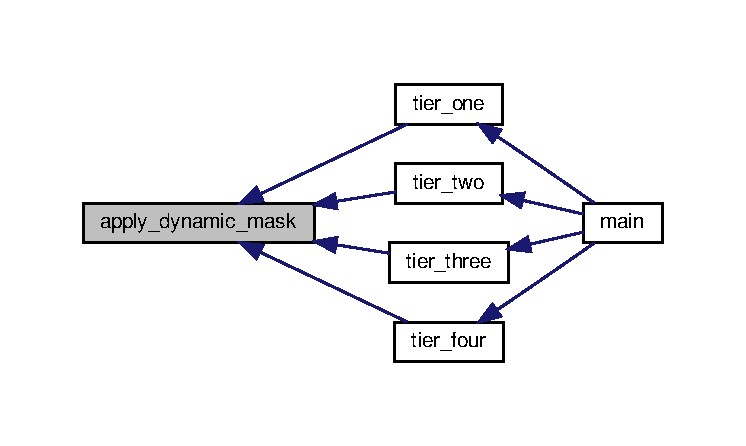
\includegraphics[width=350pt]{frame__extraction_8cpp_adb0537fa8d7c5a8932f1abc66ee3d3f3_icgraph}
\end{center}
\end{figure}
\mbox{\Hypertarget{frame__extraction_8cpp_a3fe52ab2a13802c64a500f3b3fac618c}\label{frame__extraction_8cpp_a3fe52ab2a13802c64a500f3b3fac618c}} 
\index{frame\+\_\+extraction.\+cpp@{frame\+\_\+extraction.\+cpp}!box\+\_\+data@{box\+\_\+data}}
\index{box\+\_\+data@{box\+\_\+data}!frame\+\_\+extraction.\+cpp@{frame\+\_\+extraction.\+cpp}}
\subsubsection{\texorpdfstring{box\+\_\+data()}{box\_data()}}
{\footnotesize\ttfamily static int box\+\_\+data (\begin{DoxyParamCaption}\item[{Rect}]{box,  }\item[{int}]{framecnt }\end{DoxyParamCaption})\hspace{0.3cm}{\ttfamily [static]}}


\begin{DoxyParams}{Parameters}
{\em in\+\_\+frame} & Open\+CV matrix image, 16-\/bit single depth format \\
\hline
{\em framecnt} & int of nth frame retrieved by program \\
\hline
\end{DoxyParams}
\begin{DoxyReturn}{Returns}
status 
\end{DoxyReturn}
Here is the caller graph for this function\+:\nopagebreak
\begin{figure}[H]
\begin{center}
\leavevmode
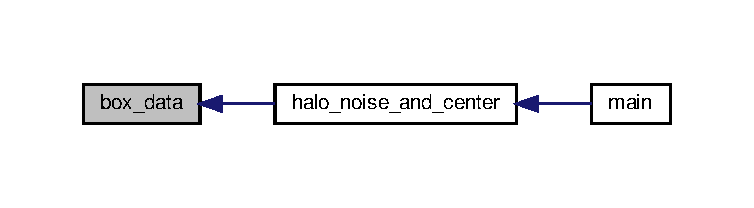
\includegraphics[width=350pt]{frame__extraction_8cpp_a3fe52ab2a13802c64a500f3b3fac618c_icgraph}
\end{center}
\end{figure}
\mbox{\Hypertarget{frame__extraction_8cpp_ab82da2f54d3288500af385f722ee691e}\label{frame__extraction_8cpp_ab82da2f54d3288500af385f722ee691e}} 
\index{frame\+\_\+extraction.\+cpp@{frame\+\_\+extraction.\+cpp}!box\+\_\+finder@{box\+\_\+finder}}
\index{box\+\_\+finder@{box\+\_\+finder}!frame\+\_\+extraction.\+cpp@{frame\+\_\+extraction.\+cpp}}
\subsubsection{\texorpdfstring{box\+\_\+finder()}{box\_finder()}}
{\footnotesize\ttfamily static int box\+\_\+finder (\begin{DoxyParamCaption}\item[{Mat}]{in\+\_\+frame,  }\item[{bool}]{do\+\_\+thresh }\end{DoxyParamCaption})\hspace{0.3cm}{\ttfamily [static]}}

This function finds the bounding box for the largest contour and reports on its properties. Stores Open\+CV Rect object bounding the largest contour (presumably the moon) to global B\+F\+\_\+\+B\+OX.


\begin{DoxyParams}{Parameters}
{\em in\+\_\+frame} & Open\+CV matrix image, 16-\/bit single depth format \\
\hline
\end{DoxyParams}
\begin{DoxyReturn}{Returns}
status 
\end{DoxyReturn}
Here is the call graph for this function\+:\nopagebreak
\begin{figure}[H]
\begin{center}
\leavevmode
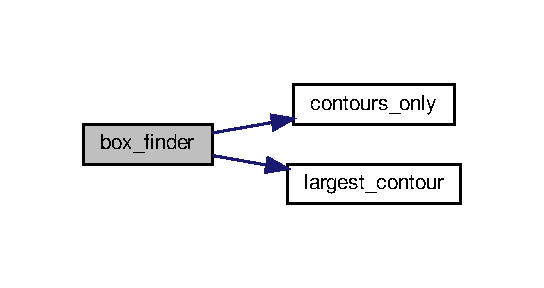
\includegraphics[width=261pt]{frame__extraction_8cpp_ab82da2f54d3288500af385f722ee691e_cgraph}
\end{center}
\end{figure}
Here is the caller graph for this function\+:\nopagebreak
\begin{figure}[H]
\begin{center}
\leavevmode
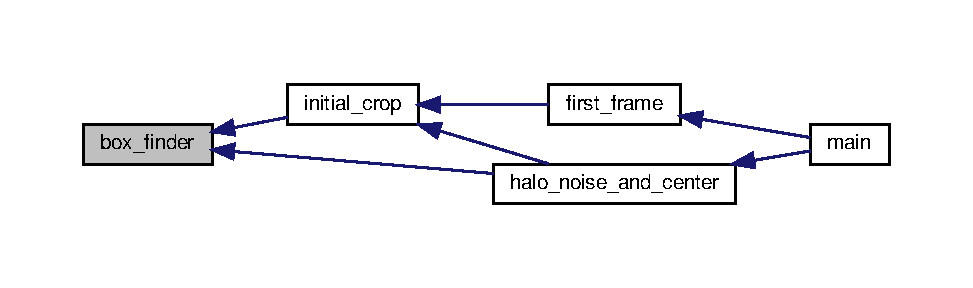
\includegraphics[width=350pt]{frame__extraction_8cpp_ab82da2f54d3288500af385f722ee691e_icgraph}
\end{center}
\end{figure}
\mbox{\Hypertarget{frame__extraction_8cpp_a579a6e5cf9846789c07a88e72ef4a7a7}\label{frame__extraction_8cpp_a579a6e5cf9846789c07a88e72ef4a7a7}} 
\index{frame\+\_\+extraction.\+cpp@{frame\+\_\+extraction.\+cpp}!concat\+\_\+tiers@{concat\+\_\+tiers}}
\index{concat\+\_\+tiers@{concat\+\_\+tiers}!frame\+\_\+extraction.\+cpp@{frame\+\_\+extraction.\+cpp}}
\subsubsection{\texorpdfstring{concat\+\_\+tiers()}{concat\_tiers()}}
{\footnotesize\ttfamily static int concat\+\_\+tiers (\begin{DoxyParamCaption}{ }\end{DoxyParamCaption})\hspace{0.3cm}{\ttfamily [static]}}

Concatenates the Tiered data files into a single file called mixed\+\_\+tiers.\+csv This requires the linux sort function to run because sorting csv in C++ ab initio is painful

\begin{DoxyReturn}{Returns}
status 
\end{DoxyReturn}
Here is the call graph for this function\+:\nopagebreak
\begin{figure}[H]
\begin{center}
\leavevmode
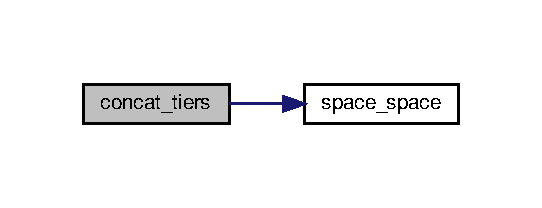
\includegraphics[width=260pt]{frame__extraction_8cpp_a579a6e5cf9846789c07a88e72ef4a7a7_cgraph}
\end{center}
\end{figure}
Here is the caller graph for this function\+:\nopagebreak
\begin{figure}[H]
\begin{center}
\leavevmode
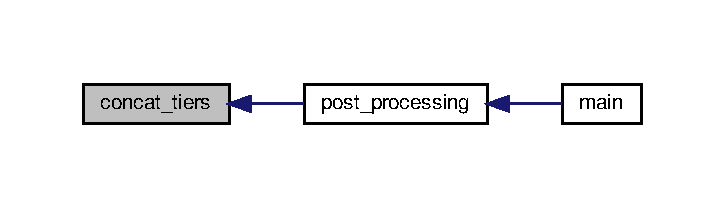
\includegraphics[width=348pt]{frame__extraction_8cpp_a579a6e5cf9846789c07a88e72ef4a7a7_icgraph}
\end{center}
\end{figure}
\mbox{\Hypertarget{frame__extraction_8cpp_a5a1b727e663ec81191fd584338c88227}\label{frame__extraction_8cpp_a5a1b727e663ec81191fd584338c88227}} 
\index{frame\+\_\+extraction.\+cpp@{frame\+\_\+extraction.\+cpp}!contours\+\_\+only@{contours\+\_\+only}}
\index{contours\+\_\+only@{contours\+\_\+only}!frame\+\_\+extraction.\+cpp@{frame\+\_\+extraction.\+cpp}}
\subsubsection{\texorpdfstring{contours\+\_\+only()}{contours\_only()}}
{\footnotesize\ttfamily static vector$<$vector$<$Point$>$ $>$ contours\+\_\+only (\begin{DoxyParamCaption}\item[{Mat}]{in\+\_\+frame }\end{DoxyParamCaption})\hspace{0.3cm}{\ttfamily [static]}}

This function returns the contours from an image. It really only needs to exist because repeatedly declaring the unused hierarchy is tedious.


\begin{DoxyParams}{Parameters}
{\em in\+\_\+frame} & Open\+CV matrix image, 16-\/bit single depth format \\
\hline
\end{DoxyParams}
\begin{DoxyReturn}{Returns}
vector of int-\/int Open\+CV Point vectors for each contour detected in the in\+\_\+frame 
\end{DoxyReturn}
Here is the caller graph for this function\+:\nopagebreak
\begin{figure}[H]
\begin{center}
\leavevmode
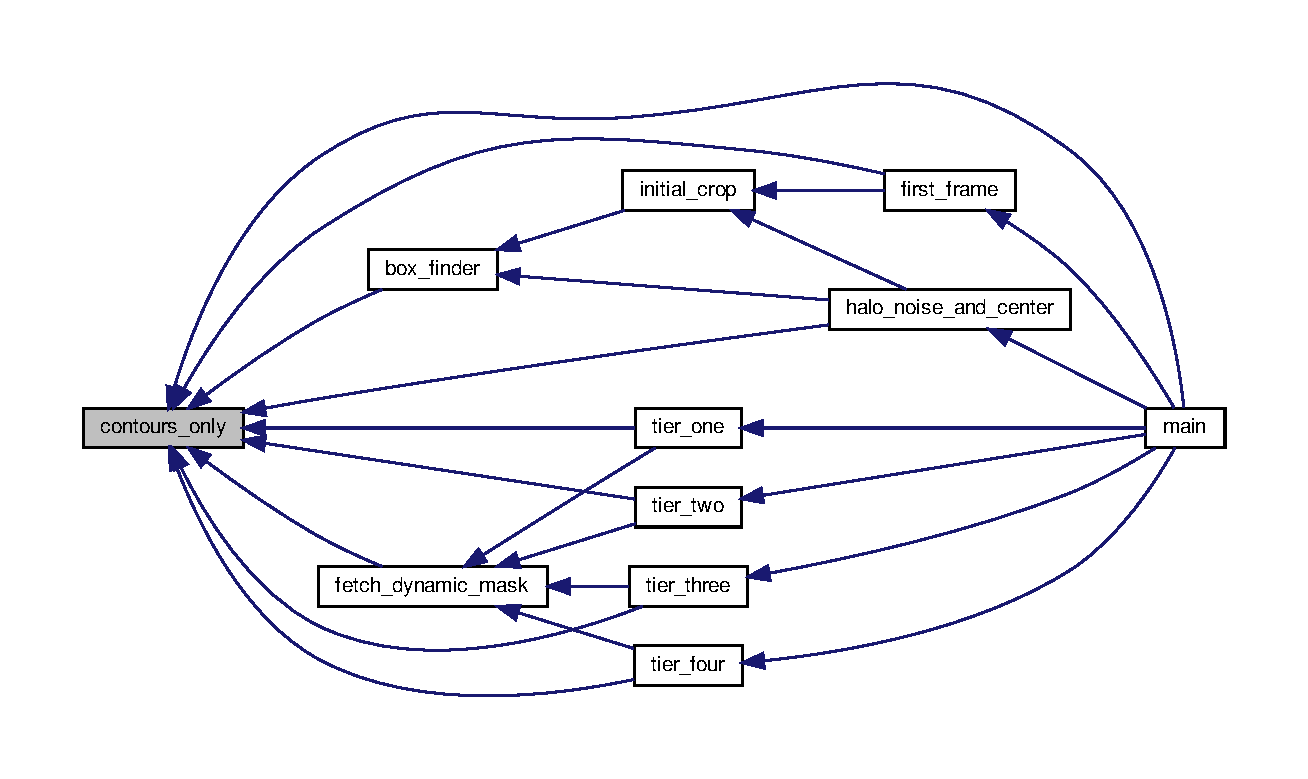
\includegraphics[width=350pt]{frame__extraction_8cpp_a5a1b727e663ec81191fd584338c88227_icgraph}
\end{center}
\end{figure}
\mbox{\Hypertarget{frame__extraction_8cpp_a19b6b938855c1060791509f406645605}\label{frame__extraction_8cpp_a19b6b938855c1060791509f406645605}} 
\index{frame\+\_\+extraction.\+cpp@{frame\+\_\+extraction.\+cpp}!corner\+\_\+matching@{corner\+\_\+matching}}
\index{corner\+\_\+matching@{corner\+\_\+matching}!frame\+\_\+extraction.\+cpp@{frame\+\_\+extraction.\+cpp}}
\subsubsection{\texorpdfstring{corner\+\_\+matching()}{corner\_matching()}}
{\footnotesize\ttfamily static Mat corner\+\_\+matching (\begin{DoxyParamCaption}\item[{Mat}]{in\+\_\+frame,  }\item[{vector$<$ Point $>$}]{contour,  }\item[{int}]{plusx,  }\item[{int}]{plusy }\end{DoxyParamCaption})\hspace{0.3cm}{\ttfamily [static]}}

If the moon cannot be centered properly using moment methods, this function is called. Here, the corner of the bounding box around the moon in the input frame is matched to the corners detected in the first frame. If the first frame of the video was centered properly, this will produce an output frame which deviates less from the intended centering function. This helps to reduce noise in when the contours are detected across all tiers. Corner matching is determined by comparison against the maximum allowable edge length declared by E\+D\+G\+E\+T\+H\+R\+E\+SH from settings.\+cfg. If this threshold is violated, corner matching will occur. Otherwise, traditional centering will occur.


\begin{DoxyParams}{Parameters}
{\em in\+\_\+frame} & Open\+CV matrix image, 16-\/bit single depth format \\
\hline
{\em contour} & Open\+CV contour, a vector of int int points \\
\hline
{\em plusx} & horizontal deviation of contour in pixels \\
\hline
{\em plusy} & vertical deviation of contour in pixels \\
\hline
\end{DoxyParams}
\begin{DoxyReturn}{Returns}
in\+\_\+frame The modified in\+\_\+frame from the input params 
\end{DoxyReturn}
Here is the call graph for this function\+:\nopagebreak
\begin{figure}[H]
\begin{center}
\leavevmode
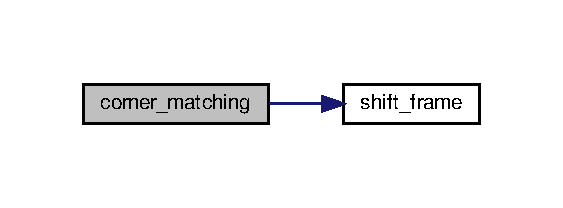
\includegraphics[width=270pt]{frame__extraction_8cpp_a19b6b938855c1060791509f406645605_cgraph}
\end{center}
\end{figure}
\mbox{\Hypertarget{frame__extraction_8cpp_a3eefea9d7b7944b3c17145bf1f42ca1f}\label{frame__extraction_8cpp_a3eefea9d7b7944b3c17145bf1f42ca1f}} 
\index{frame\+\_\+extraction.\+cpp@{frame\+\_\+extraction.\+cpp}!edge\+\_\+height@{edge\+\_\+height}}
\index{edge\+\_\+height@{edge\+\_\+height}!frame\+\_\+extraction.\+cpp@{frame\+\_\+extraction.\+cpp}}
\subsubsection{\texorpdfstring{edge\+\_\+height()}{edge\_height()}}
{\footnotesize\ttfamily static vector$<$int$>$ edge\+\_\+height (\begin{DoxyParamCaption}\item[{vector$<$ Point $>$}]{contour }\end{DoxyParamCaption})\hspace{0.3cm}{\ttfamily [static]}}

This function determines the length of the extreme left and right edges of the moon contour.


\begin{DoxyParams}{Parameters}
{\em contour} & Open\+CV contour, a vector of int int points \\
\hline
\end{DoxyParams}
\begin{DoxyReturn}{Returns}
local\+\_\+vec integer vector of the left and right edge length of the moon 
\end{DoxyReturn}
Here is the caller graph for this function\+:\nopagebreak
\begin{figure}[H]
\begin{center}
\leavevmode
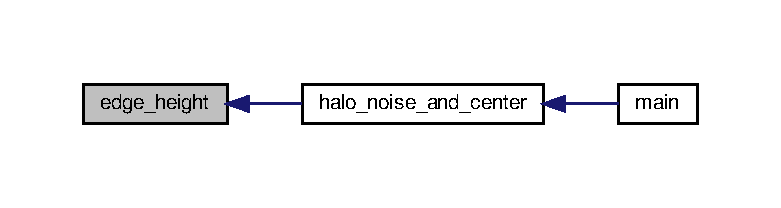
\includegraphics[width=350pt]{frame__extraction_8cpp_a3eefea9d7b7944b3c17145bf1f42ca1f_icgraph}
\end{center}
\end{figure}
\mbox{\Hypertarget{frame__extraction_8cpp_a3ac94b4b4ad476fbcdd1ac7bc26b1fe1}\label{frame__extraction_8cpp_a3ac94b4b4ad476fbcdd1ac7bc26b1fe1}} 
\index{frame\+\_\+extraction.\+cpp@{frame\+\_\+extraction.\+cpp}!edge\+\_\+width@{edge\+\_\+width}}
\index{edge\+\_\+width@{edge\+\_\+width}!frame\+\_\+extraction.\+cpp@{frame\+\_\+extraction.\+cpp}}
\subsubsection{\texorpdfstring{edge\+\_\+width()}{edge\_width()}}
{\footnotesize\ttfamily static vector$<$int$>$ edge\+\_\+width (\begin{DoxyParamCaption}\item[{vector$<$ Point $>$}]{contour }\end{DoxyParamCaption})\hspace{0.3cm}{\ttfamily [static]}}

This function determines the length of the extreme top and bottom edges of the moon contour.


\begin{DoxyParams}{Parameters}
{\em contour} & Open\+CV contour, a vector of int int points \\
\hline
\end{DoxyParams}
\begin{DoxyReturn}{Returns}
local\+\_\+vec integer vector of the top and bottom edge length of the moon 
\end{DoxyReturn}
Here is the caller graph for this function\+:\nopagebreak
\begin{figure}[H]
\begin{center}
\leavevmode
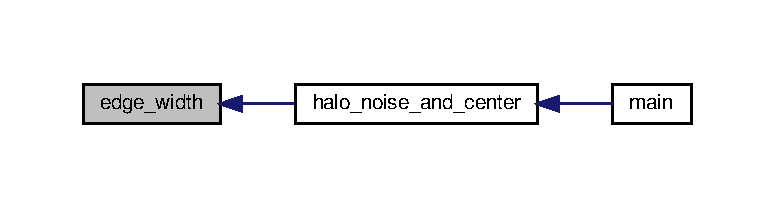
\includegraphics[width=350pt]{frame__extraction_8cpp_a3ac94b4b4ad476fbcdd1ac7bc26b1fe1_icgraph}
\end{center}
\end{figure}
\mbox{\Hypertarget{frame__extraction_8cpp_a7e01b11733281d89519fef4c5abf705c}\label{frame__extraction_8cpp_a7e01b11733281d89519fef4c5abf705c}} 
\index{frame\+\_\+extraction.\+cpp@{frame\+\_\+extraction.\+cpp}!edit\+\_\+contours\+\_\+for\+\_\+crop@{edit\+\_\+contours\+\_\+for\+\_\+crop}}
\index{edit\+\_\+contours\+\_\+for\+\_\+crop@{edit\+\_\+contours\+\_\+for\+\_\+crop}!frame\+\_\+extraction.\+cpp@{frame\+\_\+extraction.\+cpp}}
\subsubsection{\texorpdfstring{edit\+\_\+contours\+\_\+for\+\_\+crop()}{edit\_contours\_for\_crop()}}
{\footnotesize\ttfamily static int edit\+\_\+contours\+\_\+for\+\_\+crop (\begin{DoxyParamCaption}{ }\end{DoxyParamCaption})\hspace{0.3cm}{\ttfamily [static]}}

Here is the call graph for this function\+:\nopagebreak
\begin{figure}[H]
\begin{center}
\leavevmode
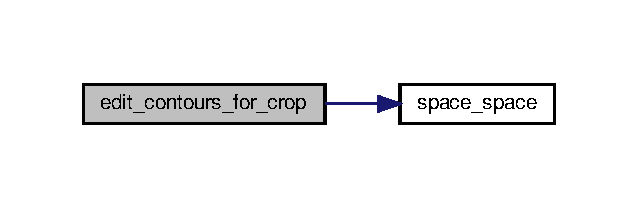
\includegraphics[width=306pt]{frame__extraction_8cpp_a7e01b11733281d89519fef4c5abf705c_cgraph}
\end{center}
\end{figure}
Here is the caller graph for this function\+:\nopagebreak
\begin{figure}[H]
\begin{center}
\leavevmode
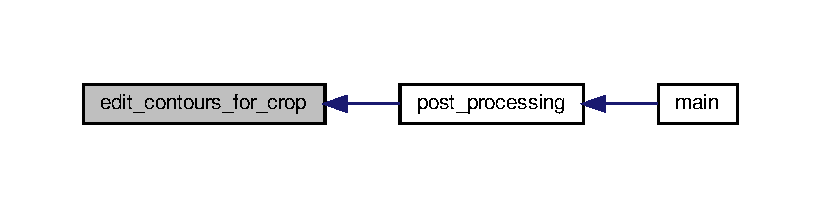
\includegraphics[width=350pt]{frame__extraction_8cpp_a7e01b11733281d89519fef4c5abf705c_icgraph}
\end{center}
\end{figure}
\mbox{\Hypertarget{frame__extraction_8cpp_a2dab519501e6a1106a8b0b2cbfd52511}\label{frame__extraction_8cpp_a2dab519501e6a1106a8b0b2cbfd52511}} 
\index{frame\+\_\+extraction.\+cpp@{frame\+\_\+extraction.\+cpp}!first\+\_\+frame@{first\+\_\+frame}}
\index{first\+\_\+frame@{first\+\_\+frame}!frame\+\_\+extraction.\+cpp@{frame\+\_\+extraction.\+cpp}}
\subsubsection{\texorpdfstring{first\+\_\+frame()}{first\_frame()}}
{\footnotesize\ttfamily static int first\+\_\+frame (\begin{DoxyParamCaption}\item[{Mat}]{in\+\_\+frame,  }\item[{int}]{framecnt }\end{DoxyParamCaption})\hspace{0.3cm}{\ttfamily [static]}}

This function is a special case of the frame preparation steps. It outputs many of the initial values which are used later (globals that start with the O\+R\+I\+G\+\_\+ template) and omits some of the masking steps not possible on the first frame.


\begin{DoxyParams}{Parameters}
{\em in\+\_\+frame} & Open\+CV matrix image, 16-\/bit single depth format \\
\hline
{\em framecnt} & int of nth frame retrieved by program \\
\hline
\end{DoxyParams}
\begin{DoxyReturn}{Returns}
in\+\_\+frame The modified in\+\_\+frame from the input params 
\end{DoxyReturn}
Here is the call graph for this function\+:\nopagebreak
\begin{figure}[H]
\begin{center}
\leavevmode
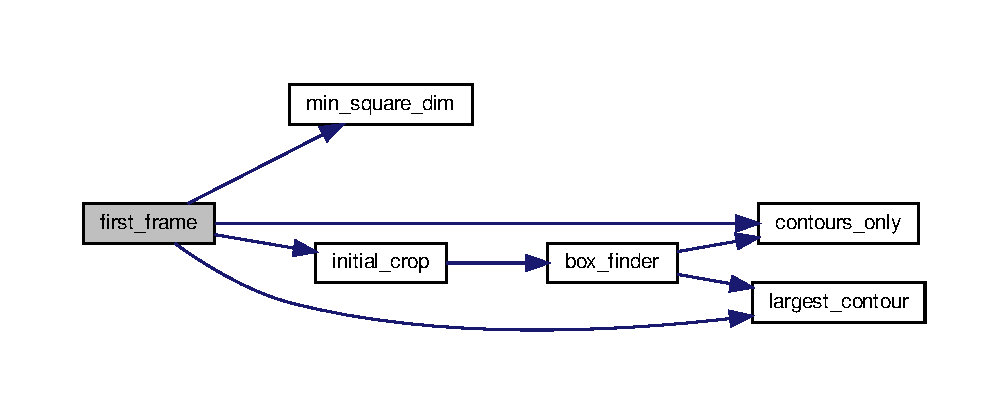
\includegraphics[width=350pt]{frame__extraction_8cpp_a2dab519501e6a1106a8b0b2cbfd52511_cgraph}
\end{center}
\end{figure}
Here is the caller graph for this function\+:\nopagebreak
\begin{figure}[H]
\begin{center}
\leavevmode
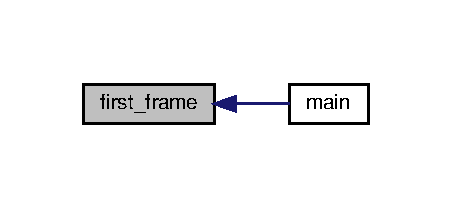
\includegraphics[width=217pt]{frame__extraction_8cpp_a2dab519501e6a1106a8b0b2cbfd52511_icgraph}
\end{center}
\end{figure}
\mbox{\Hypertarget{frame__extraction_8cpp_a272c8275ab7a0918c5e6c9acf9afda50}\label{frame__extraction_8cpp_a272c8275ab7a0918c5e6c9acf9afda50}} 
\index{frame\+\_\+extraction.\+cpp@{frame\+\_\+extraction.\+cpp}!generate\+\_\+slideshow@{generate\+\_\+slideshow}}
\index{generate\+\_\+slideshow@{generate\+\_\+slideshow}!frame\+\_\+extraction.\+cpp@{frame\+\_\+extraction.\+cpp}}
\subsubsection{\texorpdfstring{generate\+\_\+slideshow()}{generate\_slideshow()}}
{\footnotesize\ttfamily static int generate\+\_\+slideshow (\begin{DoxyParamCaption}{ }\end{DoxyParamCaption})\hspace{0.3cm}{\ttfamily [static]}}

Here is the call graph for this function\+:\nopagebreak
\begin{figure}[H]
\begin{center}
\leavevmode
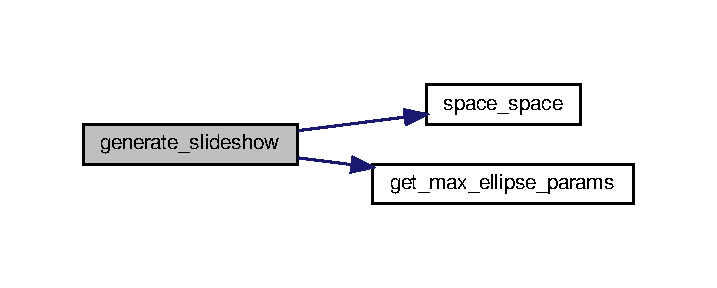
\includegraphics[width=344pt]{frame__extraction_8cpp_a272c8275ab7a0918c5e6c9acf9afda50_cgraph}
\end{center}
\end{figure}
Here is the caller graph for this function\+:\nopagebreak
\begin{figure}[H]
\begin{center}
\leavevmode
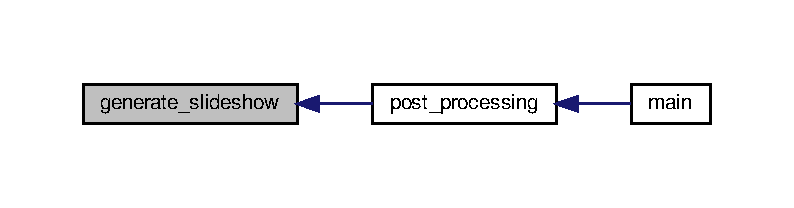
\includegraphics[width=350pt]{frame__extraction_8cpp_a272c8275ab7a0918c5e6c9acf9afda50_icgraph}
\end{center}
\end{figure}
\mbox{\Hypertarget{frame__extraction_8cpp_ae3cfeeb43523e31ac7eebd51dbf58f9c}\label{frame__extraction_8cpp_ae3cfeeb43523e31ac7eebd51dbf58f9c}} 
\index{frame\+\_\+extraction.\+cpp@{frame\+\_\+extraction.\+cpp}!get\+\_\+max\+\_\+ellipse\+\_\+params@{get\+\_\+max\+\_\+ellipse\+\_\+params}}
\index{get\+\_\+max\+\_\+ellipse\+\_\+params@{get\+\_\+max\+\_\+ellipse\+\_\+params}!frame\+\_\+extraction.\+cpp@{frame\+\_\+extraction.\+cpp}}
\subsubsection{\texorpdfstring{get\+\_\+max\+\_\+ellipse\+\_\+params()}{get\_max\_ellipse\_params()}}
{\footnotesize\ttfamily static int get\+\_\+max\+\_\+ellipse\+\_\+params (\begin{DoxyParamCaption}{ }\end{DoxyParamCaption})\hspace{0.3cm}{\ttfamily [static]}}

Determines the maximum width and height of the moon bounding box encountered in the video.

\begin{DoxyReturn}{Returns}
out\+\_\+vec a vector of ints including the maximum width and height of the moon. 
\end{DoxyReturn}
Here is the caller graph for this function\+:\nopagebreak
\begin{figure}[H]
\begin{center}
\leavevmode
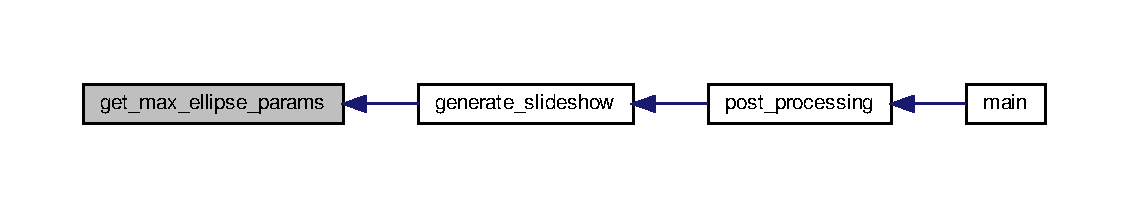
\includegraphics[width=350pt]{frame__extraction_8cpp_ae3cfeeb43523e31ac7eebd51dbf58f9c_icgraph}
\end{center}
\end{figure}
\mbox{\Hypertarget{frame__extraction_8cpp_a9c4e877be5c7a5b6c78cf2e81c09759f}\label{frame__extraction_8cpp_a9c4e877be5c7a5b6c78cf2e81c09759f}} 
\index{frame\+\_\+extraction.\+cpp@{frame\+\_\+extraction.\+cpp}!halo\+\_\+noise\+\_\+and\+\_\+center@{halo\+\_\+noise\+\_\+and\+\_\+center}}
\index{halo\+\_\+noise\+\_\+and\+\_\+center@{halo\+\_\+noise\+\_\+and\+\_\+center}!frame\+\_\+extraction.\+cpp@{frame\+\_\+extraction.\+cpp}}
\subsubsection{\texorpdfstring{halo\+\_\+noise\+\_\+and\+\_\+center()}{halo\_noise\_and\_center()}}
{\footnotesize\ttfamily static int halo\+\_\+noise\+\_\+and\+\_\+center (\begin{DoxyParamCaption}\item[{Mat}]{in\+\_\+frame,  }\item[{int}]{framecnt }\end{DoxyParamCaption})\hspace{0.3cm}{\ttfamily [static]}}

This function finds the largest contour (presumably the edge of the moon) and attempts to center the cropped image based on the centroid of the contour. It calls corner\+\_\+matching in cases where the centroid is not an appropriate method for centering. Data from this ellipse are stored in the ellipse.\+csv file. A small portion of the edge of the moon contour is removed to keep out the noisest portions. Stores modified in\+\_\+frame to H\+N\+C\+\_\+\+F\+R\+A\+ME global


\begin{DoxyParams}{Parameters}
{\em in\+\_\+frame} & Open\+CV matrix image, 16-\/bit single depth format \\
\hline
{\em framecnt} & int of nth frame retrieved by program \\
\hline
\end{DoxyParams}
\begin{DoxyReturn}{Returns}
status 
\end{DoxyReturn}
Here is the call graph for this function\+:\nopagebreak
\begin{figure}[H]
\begin{center}
\leavevmode
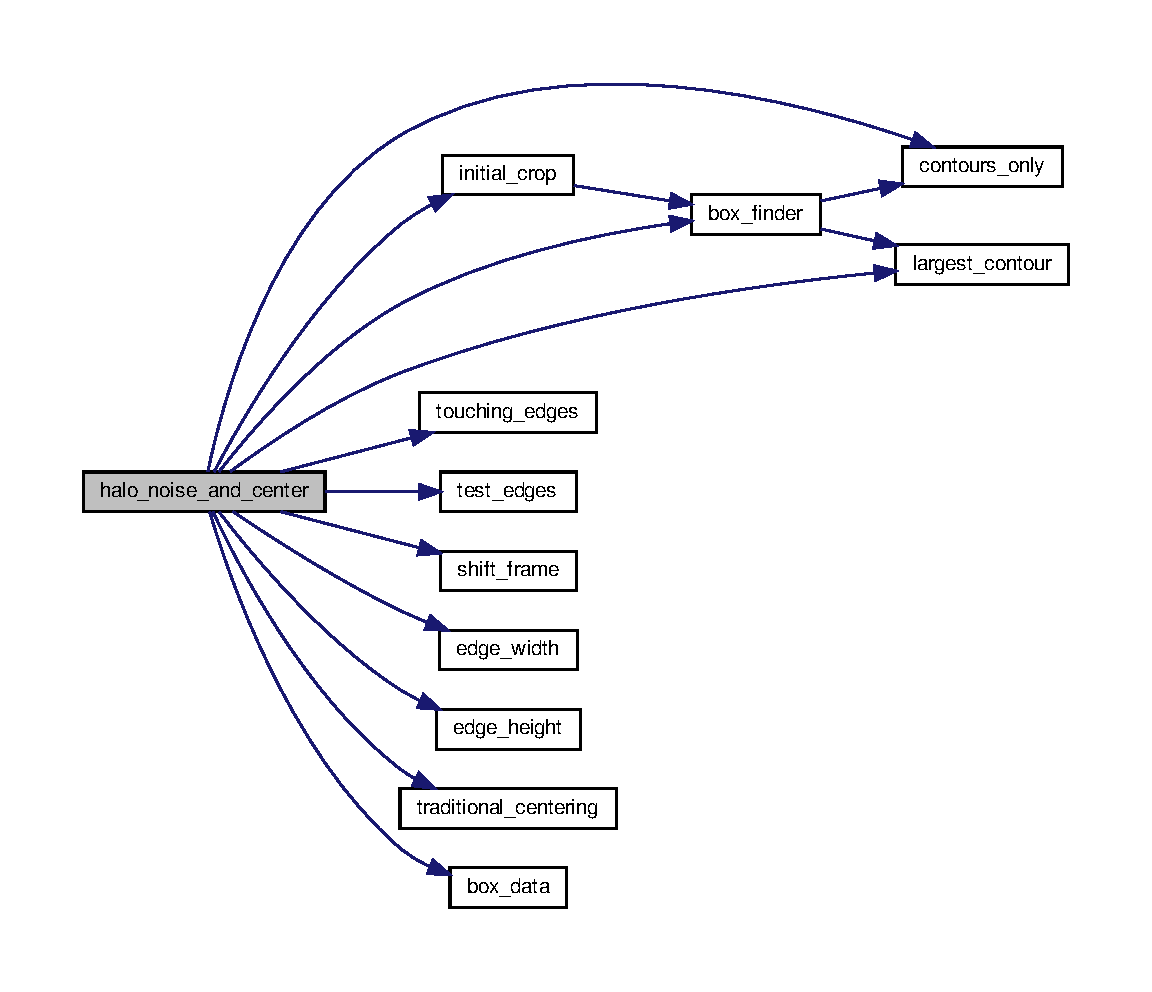
\includegraphics[width=350pt]{frame__extraction_8cpp_a9c4e877be5c7a5b6c78cf2e81c09759f_cgraph}
\end{center}
\end{figure}
Here is the caller graph for this function\+:\nopagebreak
\begin{figure}[H]
\begin{center}
\leavevmode
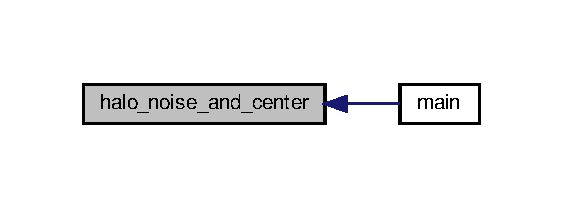
\includegraphics[width=270pt]{frame__extraction_8cpp_a9c4e877be5c7a5b6c78cf2e81c09759f_icgraph}
\end{center}
\end{figure}
\mbox{\Hypertarget{frame__extraction_8cpp_a6ebd493f01eb54e528da257db0a75e99}\label{frame__extraction_8cpp_a6ebd493f01eb54e528da257db0a75e99}} 
\index{frame\+\_\+extraction.\+cpp@{frame\+\_\+extraction.\+cpp}!initial\+\_\+crop@{initial\+\_\+crop}}
\index{initial\+\_\+crop@{initial\+\_\+crop}!frame\+\_\+extraction.\+cpp@{frame\+\_\+extraction.\+cpp}}
\subsubsection{\texorpdfstring{initial\+\_\+crop()}{initial\_crop()}}
{\footnotesize\ttfamily static int initial\+\_\+crop (\begin{DoxyParamCaption}\item[{Mat}]{in\+\_\+frame,  }\item[{int}]{framecnt }\end{DoxyParamCaption})\hspace{0.3cm}{\ttfamily [static]}}

Performs an initial rough crop on the frame. This constructs a cropped frame which contains the largest contour, but does not necessarily center the contour within the frame. That is handled by halo\+\_\+noise\+\_\+and\+\_\+center by determing whether the centering should use the corner\+\_\+matching regime or simple centroid to centroid shifting. Stores the cropped in\+\_\+frame to I\+C\+\_\+\+F\+R\+A\+ME global.


\begin{DoxyParams}{Parameters}
{\em in\+\_\+frame} & Open\+CV matrix image, 16-\/bit single depth format \\
\hline
{\em framecnt} & int of nth frame retrieved by program \\
\hline
\end{DoxyParams}
\begin{DoxyReturn}{Returns}
status 
\end{DoxyReturn}
Here is the call graph for this function\+:\nopagebreak
\begin{figure}[H]
\begin{center}
\leavevmode
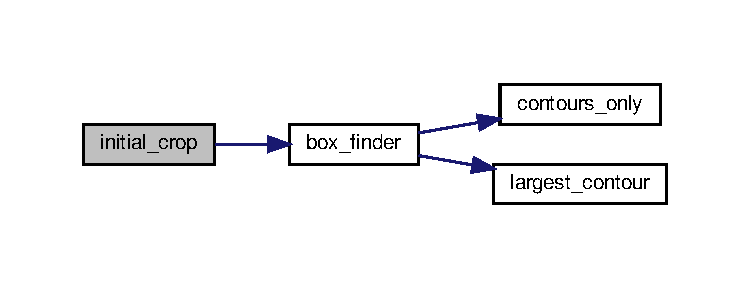
\includegraphics[width=350pt]{frame__extraction_8cpp_a6ebd493f01eb54e528da257db0a75e99_cgraph}
\end{center}
\end{figure}
Here is the caller graph for this function\+:\nopagebreak
\begin{figure}[H]
\begin{center}
\leavevmode
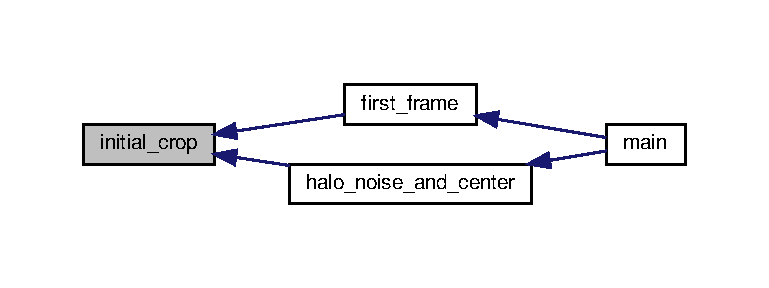
\includegraphics[width=350pt]{frame__extraction_8cpp_a6ebd493f01eb54e528da257db0a75e99_icgraph}
\end{center}
\end{figure}
\mbox{\Hypertarget{frame__extraction_8cpp_abc90f05608032b4730869812a513267f}\label{frame__extraction_8cpp_abc90f05608032b4730869812a513267f}} 
\index{frame\+\_\+extraction.\+cpp@{frame\+\_\+extraction.\+cpp}!largest\+\_\+contour@{largest\+\_\+contour}}
\index{largest\+\_\+contour@{largest\+\_\+contour}!frame\+\_\+extraction.\+cpp@{frame\+\_\+extraction.\+cpp}}
\subsubsection{\texorpdfstring{largest\+\_\+contour()}{largest\_contour()}}
{\footnotesize\ttfamily static int largest\+\_\+contour (\begin{DoxyParamCaption}\item[{vector$<$ vector$<$ Point $>$$>$}]{contours }\end{DoxyParamCaption})\hspace{0.3cm}{\ttfamily [static]}}

This function returns the index of the largest contour in a list of contours so it can be accessed in future functions.


\begin{DoxyParams}{Parameters}
{\em contours} & vector of Open\+CV vectors of int-\/int point contour edges \\
\hline
\end{DoxyParams}
\begin{DoxyReturn}{Returns}
largest\+\_\+contour\+\_\+index integer index of the largest contour in a vector of contour vectors 
\end{DoxyReturn}
Here is the caller graph for this function\+:\nopagebreak
\begin{figure}[H]
\begin{center}
\leavevmode
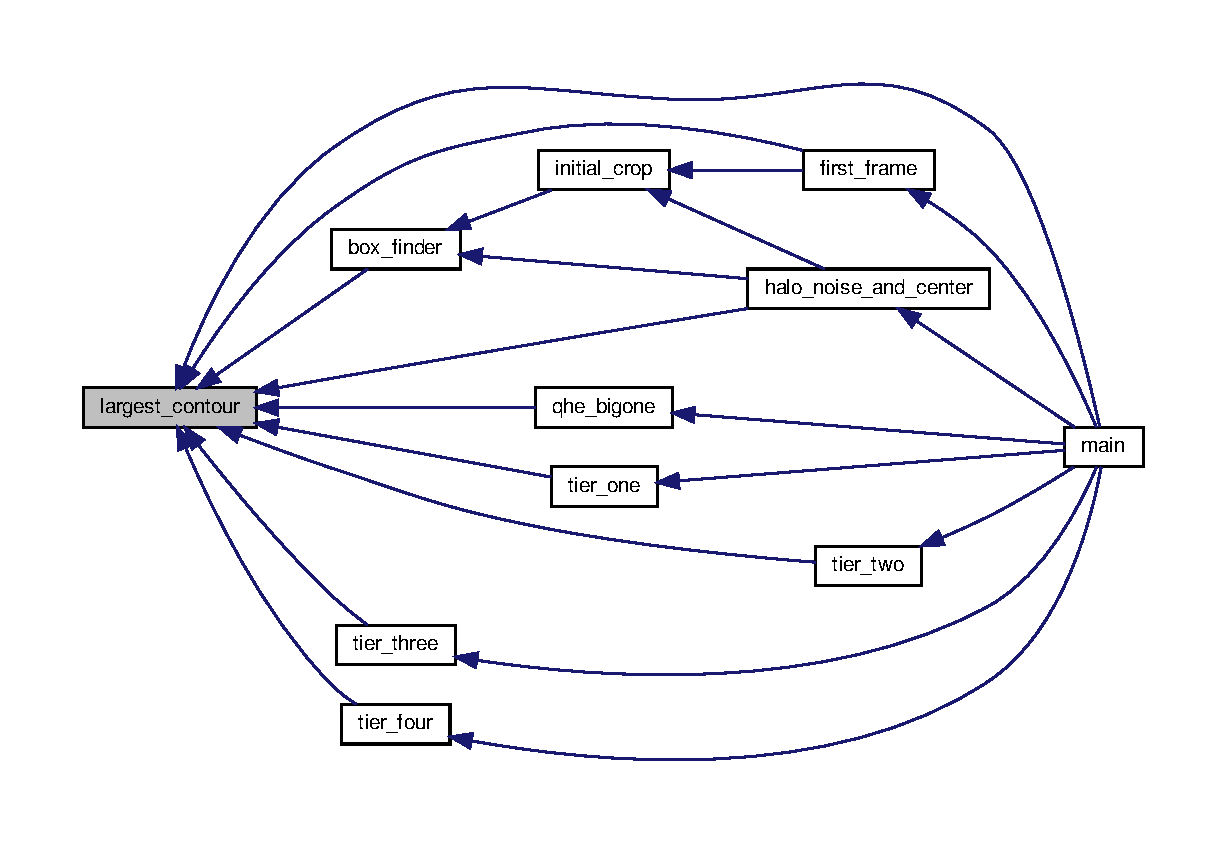
\includegraphics[width=350pt]{frame__extraction_8cpp_abc90f05608032b4730869812a513267f_icgraph}
\end{center}
\end{figure}
\mbox{\Hypertarget{frame__extraction_8cpp_a0ddf1224851353fc92bfbff6f499fa97}\label{frame__extraction_8cpp_a0ddf1224851353fc92bfbff6f499fa97}} 
\index{frame\+\_\+extraction.\+cpp@{frame\+\_\+extraction.\+cpp}!main@{main}}
\index{main@{main}!frame\+\_\+extraction.\+cpp@{frame\+\_\+extraction.\+cpp}}
\subsubsection{\texorpdfstring{main()}{main()}}
{\footnotesize\ttfamily int main (\begin{DoxyParamCaption}\item[{int}]{argc,  }\item[{char $\ast$}]{argv\mbox{[}$\,$\mbox{]} }\end{DoxyParamCaption})}

Main loop


\begin{DoxyParams}{Parameters}
{\em argc} & number of input arguments \\
\hline
{\em argv} & contents of input arguments \\
\hline
\end{DoxyParams}
\begin{DoxyReturn}{Returns}
status 
\end{DoxyReturn}
Here is the call graph for this function\+:\nopagebreak
\begin{figure}[H]
\begin{center}
\leavevmode
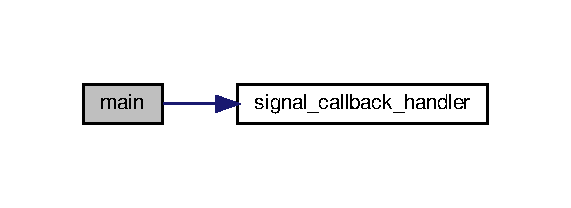
\includegraphics[width=350pt]{frame__extraction_8cpp_a0ddf1224851353fc92bfbff6f499fa97_cgraph}
\end{center}
\end{figure}
\mbox{\Hypertarget{frame__extraction_8cpp_a8b5c97016e3cad4475344f33f288bed4}\label{frame__extraction_8cpp_a8b5c97016e3cad4475344f33f288bed4}} 
\index{frame\+\_\+extraction.\+cpp@{frame\+\_\+extraction.\+cpp}!min\+\_\+square\+\_\+dim@{min\+\_\+square\+\_\+dim}}
\index{min\+\_\+square\+\_\+dim@{min\+\_\+square\+\_\+dim}!frame\+\_\+extraction.\+cpp@{frame\+\_\+extraction.\+cpp}}
\subsubsection{\texorpdfstring{min\+\_\+square\+\_\+dim()}{min\_square\_dim()}}
{\footnotesize\ttfamily static int min\+\_\+square\+\_\+dim (\begin{DoxyParamCaption}\item[{Mat}]{in\+\_\+frame }\end{DoxyParamCaption})\hspace{0.3cm}{\ttfamily [static]}}

This function stores the B\+O\+X\+S\+I\+ZE variable globally. B\+O\+X\+S\+I\+ZE is the shortest side of the input image dimensions.


\begin{DoxyParams}{Parameters}
{\em in\+\_\+frame} & Open\+CV matrix image, 16-\/bit single depth format \\
\hline
\end{DoxyParams}
\begin{DoxyReturn}{Returns}
status 
\end{DoxyReturn}
Here is the caller graph for this function\+:\nopagebreak
\begin{figure}[H]
\begin{center}
\leavevmode
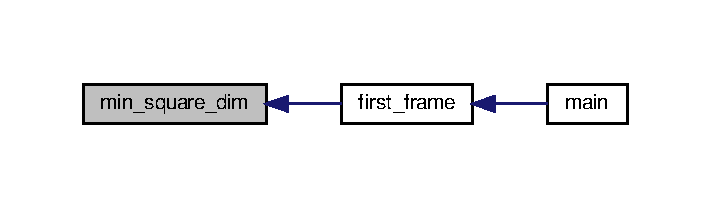
\includegraphics[width=341pt]{frame__extraction_8cpp_a8b5c97016e3cad4475344f33f288bed4_icgraph}
\end{center}
\end{figure}
\mbox{\Hypertarget{frame__extraction_8cpp_aaf7c365254fb30ce3015aded4fdf1c9d}\label{frame__extraction_8cpp_aaf7c365254fb30ce3015aded4fdf1c9d}} 
\index{frame\+\_\+extraction.\+cpp@{frame\+\_\+extraction.\+cpp}!off\+\_\+screen\+\_\+ellipse@{off\+\_\+screen\+\_\+ellipse}}
\index{off\+\_\+screen\+\_\+ellipse@{off\+\_\+screen\+\_\+ellipse}!frame\+\_\+extraction.\+cpp@{frame\+\_\+extraction.\+cpp}}
\subsubsection{\texorpdfstring{off\+\_\+screen\+\_\+ellipse()}{off\_screen\_ellipse()}}
{\footnotesize\ttfamily static int off\+\_\+screen\+\_\+ellipse (\begin{DoxyParamCaption}{ }\end{DoxyParamCaption})\hspace{0.3cm}{\ttfamily [static]}}

Simplifies the ellipse.\+csv file to only report frames where the ellispe goes off screen. Creates a new file offscreen\+\_\+moon.\+csv

\begin{DoxyReturn}{Returns}
status 
\end{DoxyReturn}
Here is the caller graph for this function\+:\nopagebreak
\begin{figure}[H]
\begin{center}
\leavevmode
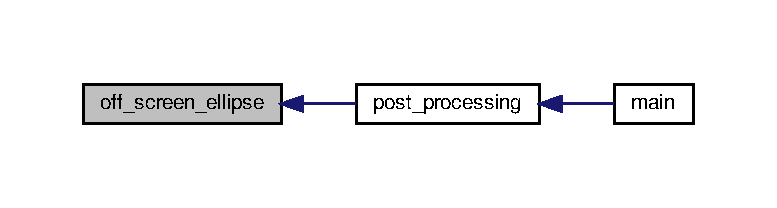
\includegraphics[width=350pt]{frame__extraction_8cpp_aaf7c365254fb30ce3015aded4fdf1c9d_icgraph}
\end{center}
\end{figure}
\mbox{\Hypertarget{frame__extraction_8cpp_ae5b18af36c3bf024f8a2dc5c4fe4242b}\label{frame__extraction_8cpp_ae5b18af36c3bf024f8a2dc5c4fe4242b}} 
\index{frame\+\_\+extraction.\+cpp@{frame\+\_\+extraction.\+cpp}!out\+\_\+frame\+\_\+gen@{out\+\_\+frame\+\_\+gen}}
\index{out\+\_\+frame\+\_\+gen@{out\+\_\+frame\+\_\+gen}!frame\+\_\+extraction.\+cpp@{frame\+\_\+extraction.\+cpp}}
\subsubsection{\texorpdfstring{out\+\_\+frame\+\_\+gen()}{out\_frame\_gen()}}
{\footnotesize\ttfamily static std\+::string out\+\_\+frame\+\_\+gen (\begin{DoxyParamCaption}\item[{int}]{framecnt }\end{DoxyParamCaption})\hspace{0.3cm}{\ttfamily [static]}}

This helper function assembles the output location for frames stored by the script.


\begin{DoxyParams}{Parameters}
{\em framecnt} & int of nth frame retrieved by program \\
\hline
\end{DoxyParams}
\begin{DoxyReturn}{Returns}
outstring the constructed path string of where to store the nth frame 
\end{DoxyReturn}
Here is the caller graph for this function\+:\nopagebreak
\begin{figure}[H]
\begin{center}
\leavevmode
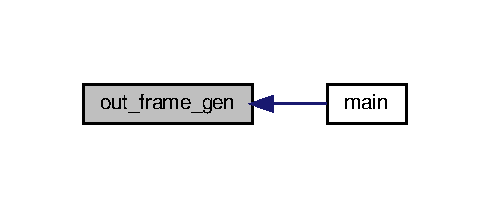
\includegraphics[width=235pt]{frame__extraction_8cpp_ae5b18af36c3bf024f8a2dc5c4fe4242b_icgraph}
\end{center}
\end{figure}
\mbox{\Hypertarget{frame__extraction_8cpp_aaee2ca25c5f0d375d48ec5b88dd6c1b3}\label{frame__extraction_8cpp_aaee2ca25c5f0d375d48ec5b88dd6c1b3}} 
\index{frame\+\_\+extraction.\+cpp@{frame\+\_\+extraction.\+cpp}!parse\+\_\+checklist@{parse\+\_\+checklist}}
\index{parse\+\_\+checklist@{parse\+\_\+checklist}!frame\+\_\+extraction.\+cpp@{frame\+\_\+extraction.\+cpp}}
\subsubsection{\texorpdfstring{parse\+\_\+checklist()}{parse\_checklist()}}
{\footnotesize\ttfamily int parse\+\_\+checklist (\begin{DoxyParamCaption}\item[{std\+::string}]{name,  }\item[{std\+::string}]{value }\end{DoxyParamCaption})}

This function handles the strings and values parsed from the settings.\+cfg file and assigns them to the global values.


\begin{DoxyParams}{Parameters}
{\em name} & String obtained while parsing the settings.\+cfg file \\
\hline
{\em value} & The value associated with name from settings.\+cfg file \\
\hline
\end{DoxyParams}
\begin{DoxyReturn}{Returns}
status 
\end{DoxyReturn}
Here is the caller graph for this function\+:\nopagebreak
\begin{figure}[H]
\begin{center}
\leavevmode
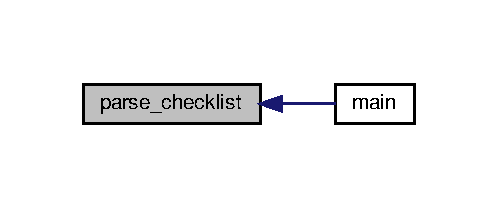
\includegraphics[width=239pt]{frame__extraction_8cpp_aaee2ca25c5f0d375d48ec5b88dd6c1b3_icgraph}
\end{center}
\end{figure}
\mbox{\Hypertarget{frame__extraction_8cpp_a34a2b5ae307c281071a717fc2d1fb0c6}\label{frame__extraction_8cpp_a34a2b5ae307c281071a717fc2d1fb0c6}} 
\index{frame\+\_\+extraction.\+cpp@{frame\+\_\+extraction.\+cpp}!post\+\_\+processing@{post\+\_\+processing}}
\index{post\+\_\+processing@{post\+\_\+processing}!frame\+\_\+extraction.\+cpp@{frame\+\_\+extraction.\+cpp}}
\subsubsection{\texorpdfstring{post\+\_\+processing()}{post\_processing()}}
{\footnotesize\ttfamily static int post\+\_\+processing (\begin{DoxyParamCaption}{ }\end{DoxyParamCaption})\hspace{0.3cm}{\ttfamily [static]}}

Holder function for processes which run after the bulk of main completes

\begin{DoxyReturn}{Returns}
status 
\end{DoxyReturn}
Here is the call graph for this function\+:\nopagebreak
\begin{figure}[H]
\begin{center}
\leavevmode
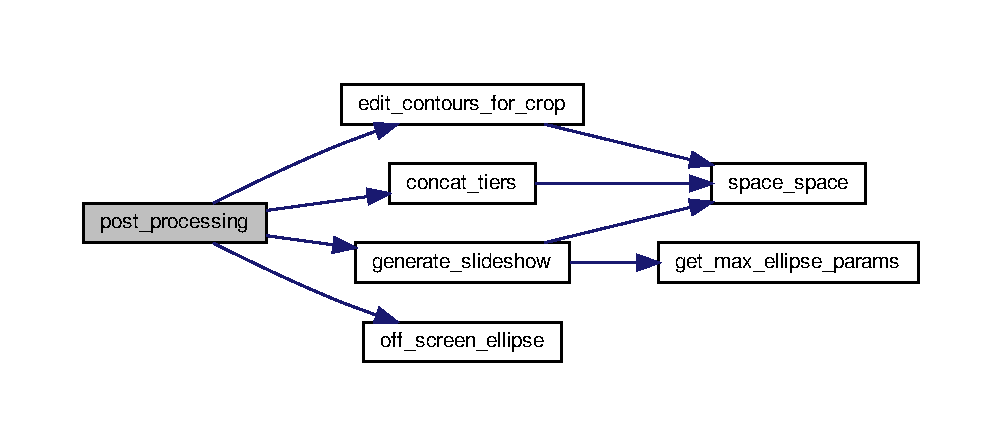
\includegraphics[width=350pt]{frame__extraction_8cpp_a34a2b5ae307c281071a717fc2d1fb0c6_cgraph}
\end{center}
\end{figure}
Here is the caller graph for this function\+:\nopagebreak
\begin{figure}[H]
\begin{center}
\leavevmode
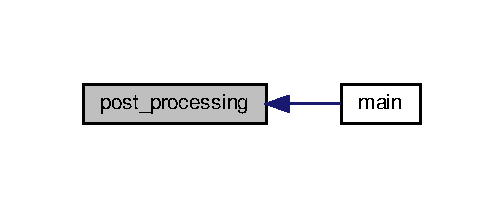
\includegraphics[width=242pt]{frame__extraction_8cpp_a34a2b5ae307c281071a717fc2d1fb0c6_icgraph}
\end{center}
\end{figure}
\mbox{\Hypertarget{frame__extraction_8cpp_a7564e59e35a0ba92812018e6ff847141}\label{frame__extraction_8cpp_a7564e59e35a0ba92812018e6ff847141}} 
\index{frame\+\_\+extraction.\+cpp@{frame\+\_\+extraction.\+cpp}!qhe\+\_\+bigone@{qhe\+\_\+bigone}}
\index{qhe\+\_\+bigone@{qhe\+\_\+bigone}!frame\+\_\+extraction.\+cpp@{frame\+\_\+extraction.\+cpp}}
\subsubsection{\texorpdfstring{qhe\+\_\+bigone()}{qhe\_bigone()}}
{\footnotesize\ttfamily static vector$<$Point$>$ qhe\+\_\+bigone (\begin{DoxyParamCaption}\item[{Mat}]{in\+\_\+frame }\end{DoxyParamCaption})\hspace{0.3cm}{\ttfamily [static]}}

Finds the largest contour within the frame after masking. Called from main thread to prevent waste of C\+PU time for each tier.


\begin{DoxyParams}{Parameters}
{\em in\+\_\+frame} & Open\+CV matrix image, 16-\/bit single depth format \\
\hline
\end{DoxyParams}
\begin{DoxyReturn}{Returns}
bigone vector of cv Points representing the largest frame in the image 
\end{DoxyReturn}
Here is the call graph for this function\+:\nopagebreak
\begin{figure}[H]
\begin{center}
\leavevmode
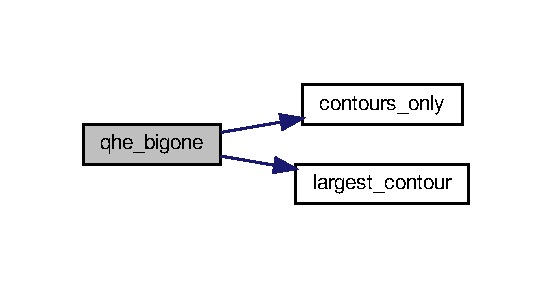
\includegraphics[width=265pt]{frame__extraction_8cpp_a7564e59e35a0ba92812018e6ff847141_cgraph}
\end{center}
\end{figure}
Here is the caller graph for this function\+:\nopagebreak
\begin{figure}[H]
\begin{center}
\leavevmode
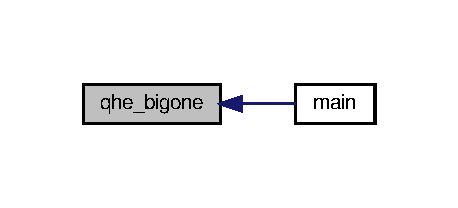
\includegraphics[width=220pt]{frame__extraction_8cpp_a7564e59e35a0ba92812018e6ff847141_icgraph}
\end{center}
\end{figure}
\mbox{\Hypertarget{frame__extraction_8cpp_ae9d9ad905beac19a35c93ee874a2c84c}\label{frame__extraction_8cpp_ae9d9ad905beac19a35c93ee874a2c84c}} 
\index{frame\+\_\+extraction.\+cpp@{frame\+\_\+extraction.\+cpp}!quiet\+\_\+halo\+\_\+elim@{quiet\+\_\+halo\+\_\+elim}}
\index{quiet\+\_\+halo\+\_\+elim@{quiet\+\_\+halo\+\_\+elim}!frame\+\_\+extraction.\+cpp@{frame\+\_\+extraction.\+cpp}}
\subsubsection{\texorpdfstring{quiet\+\_\+halo\+\_\+elim()}{quiet\_halo\_elim()}}
{\footnotesize\ttfamily static vector$<$vector$<$Point$>$ $>$ quiet\+\_\+halo\+\_\+elim (\begin{DoxyParamCaption}\item[{vector$<$ vector$<$ Point $>$$>$}]{contours,  }\item[{vector$<$ Point $>$}]{bigone }\end{DoxyParamCaption})\hspace{0.3cm}{\ttfamily [static]}}

This function removes contours which are near to the edge of the moon halo. This is a quiet kind of masking which does not alter the image, rather it quietly makes contours in violation `disappear\textquotesingle{}. The distance from the moon edge which is to be masked is determined by Q\+H\+E\+\_\+\+W\+I\+D\+TH from settings.\+cfg.


\begin{DoxyParams}{Parameters}
{\em contours} & vector of Open\+CV vectors of int-\/int point contour edges \\
\hline
{\em bigone} & vector of Opencv Points representing the largest contour from qhe\+\_\+bigone \\
\hline
\end{DoxyParams}
\begin{DoxyReturn}{Returns}
out\+\_\+contours vector of Open\+CV int-\/int Point vectors representing valid contours 
\end{DoxyReturn}
Here is the caller graph for this function\+:\nopagebreak
\begin{figure}[H]
\begin{center}
\leavevmode
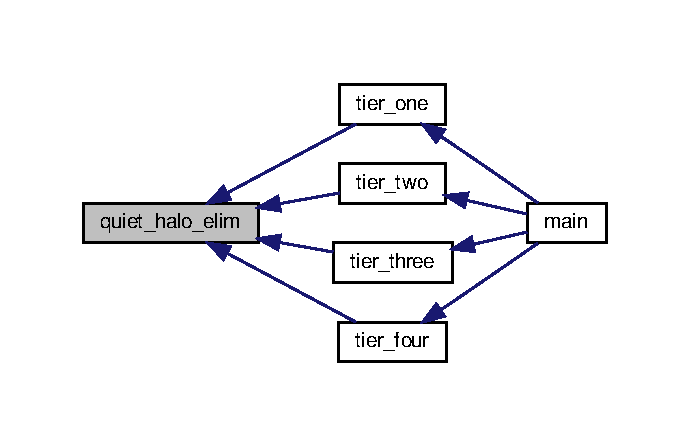
\includegraphics[width=331pt]{frame__extraction_8cpp_ae9d9ad905beac19a35c93ee874a2c84c_icgraph}
\end{center}
\end{figure}
\mbox{\Hypertarget{frame__extraction_8cpp_afae27f2c8807b9a09243b93d512b504c}\label{frame__extraction_8cpp_afae27f2c8807b9a09243b93d512b504c}} 
\index{frame\+\_\+extraction.\+cpp@{frame\+\_\+extraction.\+cpp}!shift\+\_\+frame@{shift\+\_\+frame}}
\index{shift\+\_\+frame@{shift\+\_\+frame}!frame\+\_\+extraction.\+cpp@{frame\+\_\+extraction.\+cpp}}
\subsubsection{\texorpdfstring{shift\+\_\+frame()}{shift\_frame()}}
{\footnotesize\ttfamily static Mat shift\+\_\+frame (\begin{DoxyParamCaption}\item[{Mat}]{in\+\_\+frame,  }\item[{int}]{shiftx,  }\item[{int}]{shifty }\end{DoxyParamCaption})\hspace{0.3cm}{\ttfamily [static]}}

This function performs a shifting crop of the input image based on the values shiftx and shifty. The output image will always have B\+O\+X\+O\+UT dimensions determined from the size of the original image\textquotesingle{}s shortest side.


\begin{DoxyParams}{Parameters}
{\em in\+\_\+frame} & Open\+CV matrix image, 16-\/bit single depth format \\
\hline
{\em shiftx} & number of pixels the cropped image should be shifted in the horizontal direction \\
\hline
{\em shifty} & number of pixels the cropped image should be shifted in the vertical direction \\
\hline
\end{DoxyParams}
\begin{DoxyReturn}{Returns}
in\+\_\+frame The modified in\+\_\+frame from the input params 
\end{DoxyReturn}
Here is the caller graph for this function\+:\nopagebreak
\begin{figure}[H]
\begin{center}
\leavevmode
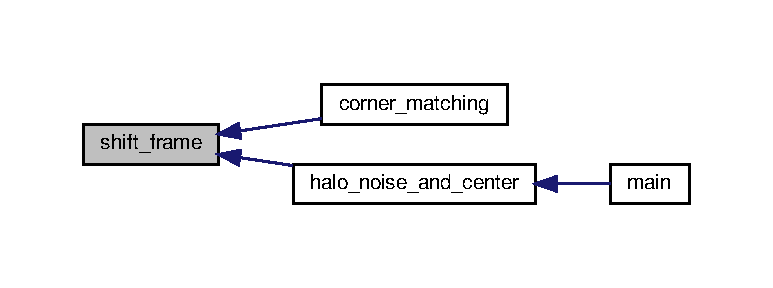
\includegraphics[width=350pt]{frame__extraction_8cpp_afae27f2c8807b9a09243b93d512b504c_icgraph}
\end{center}
\end{figure}
\mbox{\Hypertarget{frame__extraction_8cpp_a5c53b5dffc43d3917a312ade756e53ee}\label{frame__extraction_8cpp_a5c53b5dffc43d3917a312ade756e53ee}} 
\index{frame\+\_\+extraction.\+cpp@{frame\+\_\+extraction.\+cpp}!show\+\_\+usage@{show\+\_\+usage}}
\index{show\+\_\+usage@{show\+\_\+usage}!frame\+\_\+extraction.\+cpp@{frame\+\_\+extraction.\+cpp}}
\subsubsection{\texorpdfstring{show\+\_\+usage()}{show\_usage()}}
{\footnotesize\ttfamily static int show\+\_\+usage (\begin{DoxyParamCaption}\item[{string}]{name }\end{DoxyParamCaption})\hspace{0.3cm}{\ttfamily [static]}}

This is a helper function called using -\/h in terminal.


\begin{DoxyParams}{Parameters}
{\em name} & \\
\hline
\end{DoxyParams}
\begin{DoxyReturn}{Returns}
status 
\end{DoxyReturn}
Here is the caller graph for this function\+:\nopagebreak
\begin{figure}[H]
\begin{center}
\leavevmode
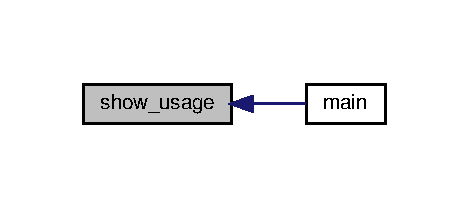
\includegraphics[width=225pt]{frame__extraction_8cpp_a5c53b5dffc43d3917a312ade756e53ee_icgraph}
\end{center}
\end{figure}
\mbox{\Hypertarget{frame__extraction_8cpp_a89a8322bea357674e81ba9cbdefe0378}\label{frame__extraction_8cpp_a89a8322bea357674e81ba9cbdefe0378}} 
\index{frame\+\_\+extraction.\+cpp@{frame\+\_\+extraction.\+cpp}!signal\+\_\+callback\+\_\+handler@{signal\+\_\+callback\+\_\+handler}}
\index{signal\+\_\+callback\+\_\+handler@{signal\+\_\+callback\+\_\+handler}!frame\+\_\+extraction.\+cpp@{frame\+\_\+extraction.\+cpp}}
\subsubsection{\texorpdfstring{signal\+\_\+callback\+\_\+handler()}{signal\_callback\_handler()}}
{\footnotesize\ttfamily void signal\+\_\+callback\+\_\+handler (\begin{DoxyParamCaption}\item[{int}]{signum }\end{DoxyParamCaption})}

This is a helper function to handle terminal signals. This shuts down the various forks properly when an interrupt is caught.


\begin{DoxyParams}{Parameters}
{\em signum} & signal number passed to this function. Only handles 2. \\
\hline
\end{DoxyParams}
Here is the caller graph for this function\+:\nopagebreak
\begin{figure}[H]
\begin{center}
\leavevmode
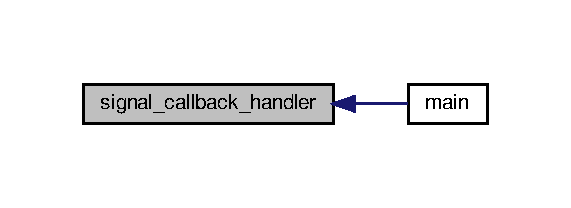
\includegraphics[width=274pt]{frame__extraction_8cpp_a89a8322bea357674e81ba9cbdefe0378_icgraph}
\end{center}
\end{figure}
\mbox{\Hypertarget{frame__extraction_8cpp_a6aa2b943656a2bdc7bbb9a4f9e1adcd1}\label{frame__extraction_8cpp_a6aa2b943656a2bdc7bbb9a4f9e1adcd1}} 
\index{frame\+\_\+extraction.\+cpp@{frame\+\_\+extraction.\+cpp}!space\+\_\+space@{space\+\_\+space}}
\index{space\+\_\+space@{space\+\_\+space}!frame\+\_\+extraction.\+cpp@{frame\+\_\+extraction.\+cpp}}
\subsubsection{\texorpdfstring{space\+\_\+space()}{space\_space()}}
{\footnotesize\ttfamily std\+::string space\+\_\+space (\begin{DoxyParamCaption}\item[{std\+::string}]{instring }\end{DoxyParamCaption})}

This helper function handles spaces in user paths.


\begin{DoxyParams}{Parameters}
{\em instring} & the input string \\
\hline
\end{DoxyParams}
\begin{DoxyReturn}{Returns}
outstring the corrected string 
\end{DoxyReturn}
Here is the caller graph for this function\+:\nopagebreak
\begin{figure}[H]
\begin{center}
\leavevmode
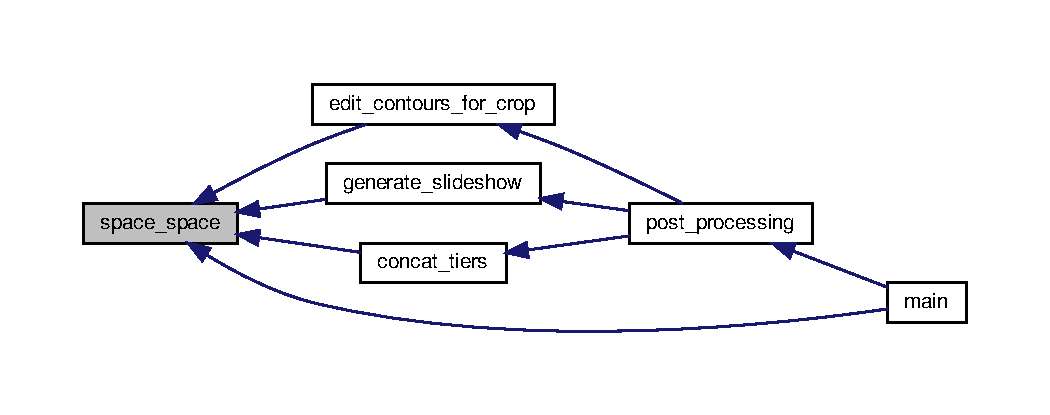
\includegraphics[width=350pt]{frame__extraction_8cpp_a6aa2b943656a2bdc7bbb9a4f9e1adcd1_icgraph}
\end{center}
\end{figure}
\mbox{\Hypertarget{frame__extraction_8cpp_a0053c162fe33c7a2536d9b87dc7f3260}\label{frame__extraction_8cpp_a0053c162fe33c7a2536d9b87dc7f3260}} 
\index{frame\+\_\+extraction.\+cpp@{frame\+\_\+extraction.\+cpp}!tail@{tail}}
\index{tail@{tail}!frame\+\_\+extraction.\+cpp@{frame\+\_\+extraction.\+cpp}}
\subsubsection{\texorpdfstring{tail()}{tail()}}
{\footnotesize\ttfamily std\+::string tail (\begin{DoxyParamCaption}\item[{std\+::string const \&}]{source,  }\item[{size\+\_\+t const}]{length }\end{DoxyParamCaption})}

Get the last n characters of a string. Handles incorrectly sized searches.


\begin{DoxyParams}{Parameters}
{\em source} & Input string \\
\hline
{\em length} & Number of characters from the back to return \\
\hline
\end{DoxyParams}
Here is the caller graph for this function\+:\nopagebreak
\begin{figure}[H]
\begin{center}
\leavevmode
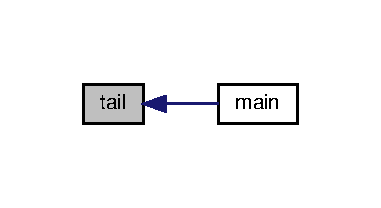
\includegraphics[width=183pt]{frame__extraction_8cpp_a0053c162fe33c7a2536d9b87dc7f3260_icgraph}
\end{center}
\end{figure}
\mbox{\Hypertarget{frame__extraction_8cpp_a5ef2b91877d44dada29b478b53744af6}\label{frame__extraction_8cpp_a5ef2b91877d44dada29b478b53744af6}} 
\index{frame\+\_\+extraction.\+cpp@{frame\+\_\+extraction.\+cpp}!test\+\_\+edges@{test\+\_\+edges}}
\index{test\+\_\+edges@{test\+\_\+edges}!frame\+\_\+extraction.\+cpp@{frame\+\_\+extraction.\+cpp}}
\subsubsection{\texorpdfstring{test\+\_\+edges()}{test\_edges()}}
{\footnotesize\ttfamily static vector$<$int$>$ test\+\_\+edges (\begin{DoxyParamCaption}\item[{Mat}]{in\+\_\+frame,  }\item[{vector$<$ Point $>$}]{contour,  }\item[{int}]{te\+\_\+ret }\end{DoxyParamCaption})\hspace{0.3cm}{\ttfamily [static]}}

This function tests the moon contour to determine the degree of shift required to center it in a frame.


\begin{DoxyParams}{Parameters}
{\em in\+\_\+frame} & Open\+CV matrix image, 16-\/bit single depth format \\
\hline
{\em contour} & Open\+CV contour, a vector of int int points \\
\hline
\end{DoxyParams}
\begin{DoxyReturn}{Returns}
outplus integer vector of horizontal and vertical deviation of the primary contour 
\end{DoxyReturn}
Here is the caller graph for this function\+:\nopagebreak
\begin{figure}[H]
\begin{center}
\leavevmode
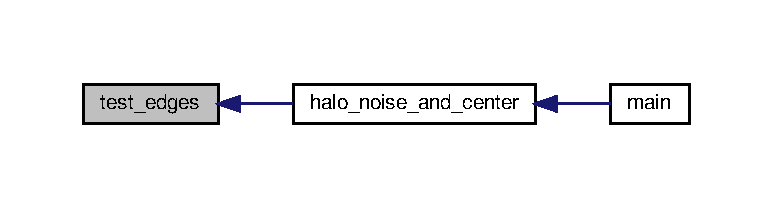
\includegraphics[width=350pt]{frame__extraction_8cpp_a5ef2b91877d44dada29b478b53744af6_icgraph}
\end{center}
\end{figure}
\mbox{\Hypertarget{frame__extraction_8cpp_abf1a9d948afc821690ec8c5c13dcee07}\label{frame__extraction_8cpp_abf1a9d948afc821690ec8c5c13dcee07}} 
\index{frame\+\_\+extraction.\+cpp@{frame\+\_\+extraction.\+cpp}!tier\+\_\+four@{tier\+\_\+four}}
\index{tier\+\_\+four@{tier\+\_\+four}!frame\+\_\+extraction.\+cpp@{frame\+\_\+extraction.\+cpp}}
\subsubsection{\texorpdfstring{tier\+\_\+four()}{tier\_four()}}
{\footnotesize\ttfamily int tier\+\_\+four (\begin{DoxyParamCaption}\item[{int}]{framecnt,  }\item[{Mat}]{in\+\_\+frame,  }\item[{Mat}]{old\+\_\+frame,  }\item[{vector$<$ Point $>$}]{bigone }\end{DoxyParamCaption})}

This is the fourth pass to detect valid contours in a frame. The parameters of the function are set in the T4 section of settings.\+cfg. This is the Un\+Canny method for detecting motion. The steps are essentially the backward operation of the steps taken during Canny filtering. The current frame is subtracted from the previous frame, and this output is threholded. The thresholded image is then passed through directional Sobel filters to separate the x and y components. These components are squared, added to each other, and square rooted. The output is rescaled to match the input value ranges, and a Gaussian blur is applied. Since this output is messy, the blurry image is processed using Zhang-\/\+Suen thinning to get distinct edges. Any details lost between the blurring and thinning steps reduce noise. Contours are then detected in the normal way.


\begin{DoxyParams}{Parameters}
{\em framecnt} & int of nth frame retrieved by program \\
\hline
{\em in\+\_\+frame} & Open\+CV matrix image, 16-\/bit single depth format \\
\hline
{\em old\+\_\+frame} & Open\+CV matrix image, 16-\/bit single depth format, stored from previous cycle \\
\hline
{\em bigone} & vector of Opencv Points representing the largest contour from qhe\+\_\+bigone \\
\hline
\end{DoxyParams}
\begin{DoxyReturn}{Returns}
status 
\end{DoxyReturn}
Here is the call graph for this function\+:\nopagebreak
\begin{figure}[H]
\begin{center}
\leavevmode
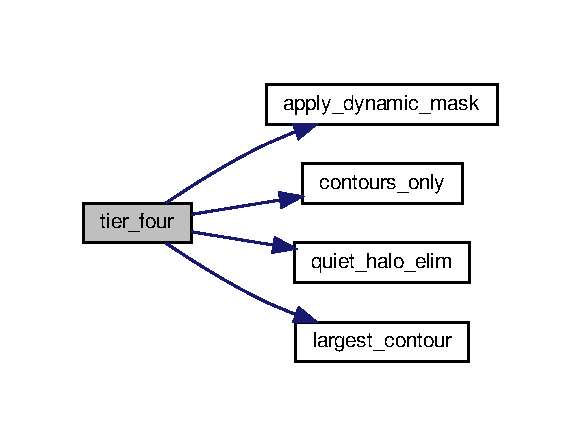
\includegraphics[width=279pt]{frame__extraction_8cpp_abf1a9d948afc821690ec8c5c13dcee07_cgraph}
\end{center}
\end{figure}
Here is the caller graph for this function\+:\nopagebreak
\begin{figure}[H]
\begin{center}
\leavevmode
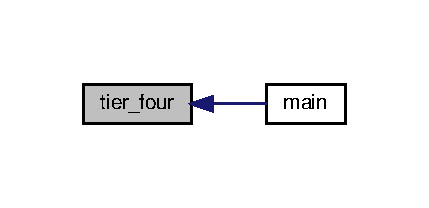
\includegraphics[width=206pt]{frame__extraction_8cpp_abf1a9d948afc821690ec8c5c13dcee07_icgraph}
\end{center}
\end{figure}
\mbox{\Hypertarget{frame__extraction_8cpp_a26d746fc8b9f07ddace0bc9eef68c1c1}\label{frame__extraction_8cpp_a26d746fc8b9f07ddace0bc9eef68c1c1}} 
\index{frame\+\_\+extraction.\+cpp@{frame\+\_\+extraction.\+cpp}!tier\+\_\+one@{tier\+\_\+one}}
\index{tier\+\_\+one@{tier\+\_\+one}!frame\+\_\+extraction.\+cpp@{frame\+\_\+extraction.\+cpp}}
\subsubsection{\texorpdfstring{tier\+\_\+one()}{tier\_one()}}
{\footnotesize\ttfamily int tier\+\_\+one (\begin{DoxyParamCaption}\item[{int}]{framecnt,  }\item[{Mat}]{in\+\_\+frame,  }\item[{vector$<$ Point $>$}]{bigone }\end{DoxyParamCaption})}

This is the first pass to detect valid contours in a frame. The parameters of the function are set in the T1 section of settings.\+cfg. Contours are detected based on a relatively strict Open\+CV adaptive\+Threshold function. These should be gauranteed \char`\"{}hits\char`\"{}.


\begin{DoxyParams}{Parameters}
{\em framecnt} & int of nth frame retrieved by program \\
\hline
{\em in\+\_\+frame} & Open\+CV matrix image, 16-\/bit single depth format \\
\hline
{\em bigone} & vector of Opencv Points representing the largest contour from qhe\+\_\+bigone \\
\hline
\end{DoxyParams}
\begin{DoxyReturn}{Returns}
status 
\end{DoxyReturn}
Here is the call graph for this function\+:\nopagebreak
\begin{figure}[H]
\begin{center}
\leavevmode
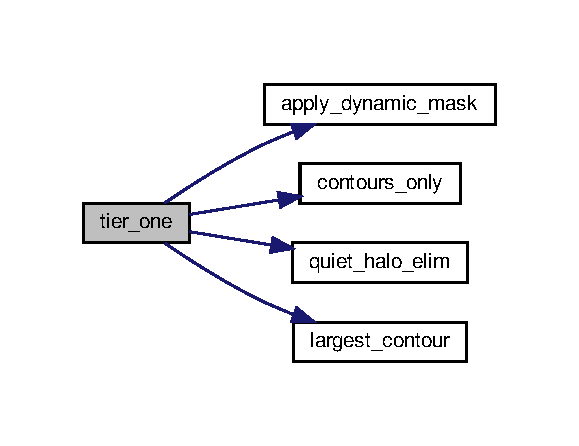
\includegraphics[width=278pt]{frame__extraction_8cpp_a26d746fc8b9f07ddace0bc9eef68c1c1_cgraph}
\end{center}
\end{figure}
Here is the caller graph for this function\+:\nopagebreak
\begin{figure}[H]
\begin{center}
\leavevmode
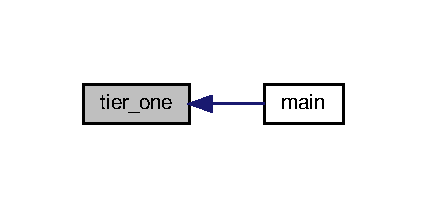
\includegraphics[width=205pt]{frame__extraction_8cpp_a26d746fc8b9f07ddace0bc9eef68c1c1_icgraph}
\end{center}
\end{figure}
\mbox{\Hypertarget{frame__extraction_8cpp_a001a4318d62e5fcdb8b910d1f4dbab36}\label{frame__extraction_8cpp_a001a4318d62e5fcdb8b910d1f4dbab36}} 
\index{frame\+\_\+extraction.\+cpp@{frame\+\_\+extraction.\+cpp}!tier\+\_\+three@{tier\+\_\+three}}
\index{tier\+\_\+three@{tier\+\_\+three}!frame\+\_\+extraction.\+cpp@{frame\+\_\+extraction.\+cpp}}
\subsubsection{\texorpdfstring{tier\+\_\+three()}{tier\_three()}}
{\footnotesize\ttfamily int tier\+\_\+three (\begin{DoxyParamCaption}\item[{int}]{framecnt,  }\item[{Mat}]{in\+\_\+frame,  }\item[{Mat}]{old\+\_\+frame,  }\item[{vector$<$ Point $>$}]{bigone }\end{DoxyParamCaption})}

This is the third pass to detect valid contours in a frame. The parameters of the function are set in the T3 section of settings.\+cfg. The detector performs an isotropic Laplacian on the current frame and the previous frame (settings.\+cfg can be modified for anisotropic Laplacian). The outputs are blurred and recombined. Values passing a cutoff threshold are retained and the contours are detected.


\begin{DoxyParams}{Parameters}
{\em framecnt} & int of nth frame retrieved by program \\
\hline
{\em in\+\_\+frame} & Open\+CV matrix image, 16-\/bit single depth format \\
\hline
{\em old\+\_\+frame} & Open\+CV matrix image, 16-\/bit single depth format, stored from previous cycle \\
\hline
{\em bigone} & vector of Opencv Points representing the largest contour from qhe\+\_\+bigone \\
\hline
\end{DoxyParams}
\begin{DoxyReturn}{Returns}
status 
\end{DoxyReturn}
Here is the call graph for this function\+:\nopagebreak
\begin{figure}[H]
\begin{center}
\leavevmode
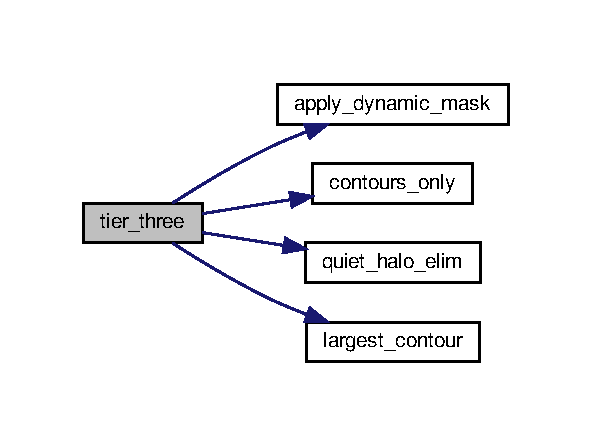
\includegraphics[width=284pt]{frame__extraction_8cpp_a001a4318d62e5fcdb8b910d1f4dbab36_cgraph}
\end{center}
\end{figure}
Here is the caller graph for this function\+:\nopagebreak
\begin{figure}[H]
\begin{center}
\leavevmode
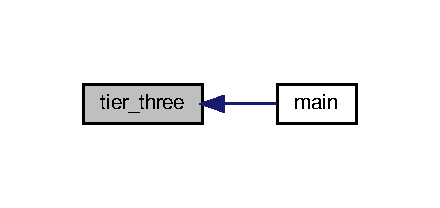
\includegraphics[width=211pt]{frame__extraction_8cpp_a001a4318d62e5fcdb8b910d1f4dbab36_icgraph}
\end{center}
\end{figure}
\mbox{\Hypertarget{frame__extraction_8cpp_ad1e0683d8ff18ab579fbb2fcce6da1cc}\label{frame__extraction_8cpp_ad1e0683d8ff18ab579fbb2fcce6da1cc}} 
\index{frame\+\_\+extraction.\+cpp@{frame\+\_\+extraction.\+cpp}!tier\+\_\+two@{tier\+\_\+two}}
\index{tier\+\_\+two@{tier\+\_\+two}!frame\+\_\+extraction.\+cpp@{frame\+\_\+extraction.\+cpp}}
\subsubsection{\texorpdfstring{tier\+\_\+two()}{tier\_two()}}
{\footnotesize\ttfamily int tier\+\_\+two (\begin{DoxyParamCaption}\item[{int}]{framecnt,  }\item[{Mat}]{in\+\_\+frame,  }\item[{vector$<$ Point $>$}]{bigone }\end{DoxyParamCaption})}

This is the second pass to detect valid contours in a frame. The parameters of the function are set in the T2 section of settings.\+cfg. Contours are detected based on a relatively loose Open\+CV adaptive\+Threshold function.


\begin{DoxyParams}{Parameters}
{\em framecnt} & int of nth frame retrieved by program \\
\hline
{\em in\+\_\+frame} & Open\+CV matrix image, 16-\/bit single depth format \\
\hline
{\em bigone} & vector of Opencv Points representing the largest contour from qhe\+\_\+bigone \\
\hline
\end{DoxyParams}
\begin{DoxyReturn}{Returns}
status 
\end{DoxyReturn}
Here is the call graph for this function\+:\nopagebreak
\begin{figure}[H]
\begin{center}
\leavevmode
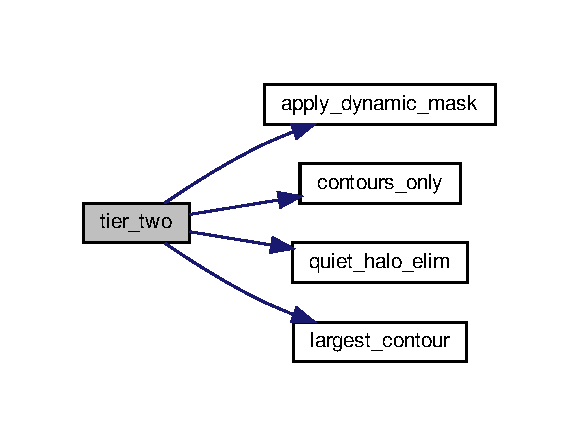
\includegraphics[width=278pt]{frame__extraction_8cpp_ad1e0683d8ff18ab579fbb2fcce6da1cc_cgraph}
\end{center}
\end{figure}
Here is the caller graph for this function\+:\nopagebreak
\begin{figure}[H]
\begin{center}
\leavevmode
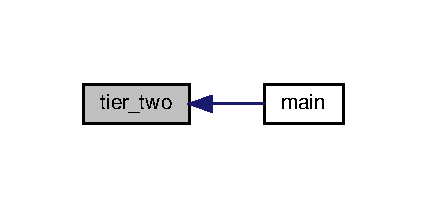
\includegraphics[width=205pt]{frame__extraction_8cpp_ad1e0683d8ff18ab579fbb2fcce6da1cc_icgraph}
\end{center}
\end{figure}
\mbox{\Hypertarget{frame__extraction_8cpp_a032ee30a958a27cdb3d5b419953ab584}\label{frame__extraction_8cpp_a032ee30a958a27cdb3d5b419953ab584}} 
\index{frame\+\_\+extraction.\+cpp@{frame\+\_\+extraction.\+cpp}!touching\+\_\+edges@{touching\+\_\+edges}}
\index{touching\+\_\+edges@{touching\+\_\+edges}!frame\+\_\+extraction.\+cpp@{frame\+\_\+extraction.\+cpp}}
\subsubsection{\texorpdfstring{touching\+\_\+edges()}{touching\_edges()}}
{\footnotesize\ttfamily static int touching\+\_\+edges (\begin{DoxyParamCaption}\item[{Mat}]{in\+\_\+frame,  }\item[{vector$<$ Point $>$}]{contour }\end{DoxyParamCaption})\hspace{0.3cm}{\ttfamily [static]}}

This function tests the input contour boundaries against the boundaries of the frame. It returns a integer value representing the edge(s) which is/are touched by the contour. If no edges are touched, this function returns zero. A negative return value indicates error. Here is a table of potential return values\+:
\begin{DoxyItemize}
\item -\/1 \+: error status
\item 0 \+: no edge touching
\item 1 \+: touching left edge only
\item 2 \+: touching right edge only
\item 3 \+: touching top and left edge
\item 4 \+: touching bottom and left edge
\item 5 \+: touching top and right edge
\item 6 \+: touching bottom and right edge
\end{DoxyItemize}


\begin{DoxyParams}{Parameters}
{\em in\+\_\+frame} & Open\+CV matrix image, 16-\/bit single depth format \\
\hline
{\em contour} & Open\+CV contour, a vector of int int points \\
\hline
\end{DoxyParams}
\begin{DoxyReturn}{Returns}
touching\+\_\+status an integer value representing if and which edge of the frame is touched by the contour. Returns negative status values if something went wrong. 
\end{DoxyReturn}
Here is the caller graph for this function\+:\nopagebreak
\begin{figure}[H]
\begin{center}
\leavevmode
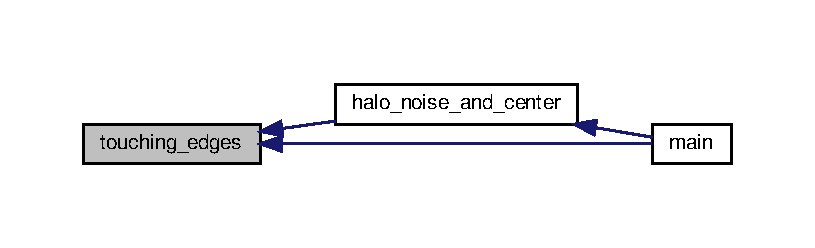
\includegraphics[width=350pt]{frame__extraction_8cpp_a032ee30a958a27cdb3d5b419953ab584_icgraph}
\end{center}
\end{figure}
\mbox{\Hypertarget{frame__extraction_8cpp_a8f336c75968d8ab7d3aa3c5c8ff74dbb}\label{frame__extraction_8cpp_a8f336c75968d8ab7d3aa3c5c8ff74dbb}} 
\index{frame\+\_\+extraction.\+cpp@{frame\+\_\+extraction.\+cpp}!traditional\+\_\+centering@{traditional\+\_\+centering}}
\index{traditional\+\_\+centering@{traditional\+\_\+centering}!frame\+\_\+extraction.\+cpp@{frame\+\_\+extraction.\+cpp}}
\subsubsection{\texorpdfstring{traditional\+\_\+centering()}{traditional\_centering()}}
{\footnotesize\ttfamily static Mat traditional\+\_\+centering (\begin{DoxyParamCaption}\item[{Mat}]{in\+\_\+frame,  }\item[{vector$<$ vector$<$ Point $>$$>$}]{contours,  }\item[{int}]{largest,  }\item[{Rect}]{box }\end{DoxyParamCaption})\hspace{0.3cm}{\ttfamily [static]}}

Here is the caller graph for this function\+:\nopagebreak
\begin{figure}[H]
\begin{center}
\leavevmode
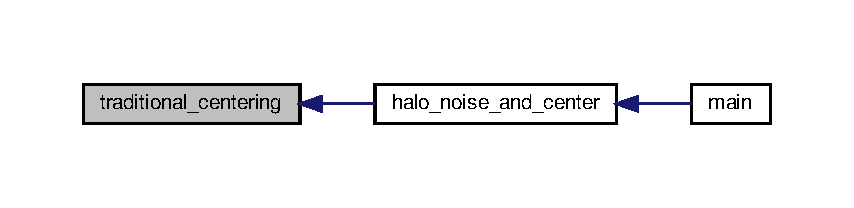
\includegraphics[width=350pt]{frame__extraction_8cpp_a8f336c75968d8ab7d3aa3c5c8ff74dbb_icgraph}
\end{center}
\end{figure}

\hypertarget{frame__extraction_8hpp}{}\section{frame\+\_\+extraction.\+hpp File Reference}
\label{frame__extraction_8hpp}\index{frame\+\_\+extraction.\+hpp@{frame\+\_\+extraction.\+hpp}}
{\ttfamily \#include $<$algorithm$>$}\newline
{\ttfamily \#include $<$ctime$>$}\newline
{\ttfamily \#include $<$errno.\+h$>$}\newline
{\ttfamily \#include $<$tgmath.\+h$>$}\newline
{\ttfamily \#include $<$fcntl.\+h$>$}\newline
{\ttfamily \#include $<$fstream$>$}\newline
{\ttfamily \#include $<$iostream$>$}\newline
{\ttfamily \#include $<$numeric$>$}\newline
{\ttfamily \#include $<$pthread.\+h$>$}\newline
{\ttfamily \#include $<$signal.\+h$>$}\newline
{\ttfamily \#include $<$stdlib.\+h$>$}\newline
{\ttfamily \#include $<$sys/ipc.\+h$>$}\newline
{\ttfamily \#include $<$sys/shm.\+h$>$}\newline
{\ttfamily \#include $<$sys/mman.\+h$>$}\newline
{\ttfamily \#include $<$sys/wait.\+h$>$}\newline
{\ttfamily \#include $<$tuple$>$}\newline
{\ttfamily \#include $<$unistd.\+h$>$}\newline
{\ttfamily \#include $<$typeinfo$>$}\newline
{\ttfamily \#include $<$regex$>$}\newline
{\ttfamily \#include $<$string$>$}\newline
{\ttfamily \#include $<$experimental/filesystem$>$}\newline
{\ttfamily \#include $<$vector$>$}\newline
{\ttfamily \#include \char`\"{}opencv2/opencv.\+hpp\char`\"{}}\newline
{\ttfamily \#include \char`\"{}opencv2/ximgproc.\+hpp\char`\"{}}\newline
Include dependency graph for frame\+\_\+extraction.\+hpp\+:\nopagebreak
\begin{figure}[H]
\begin{center}
\leavevmode
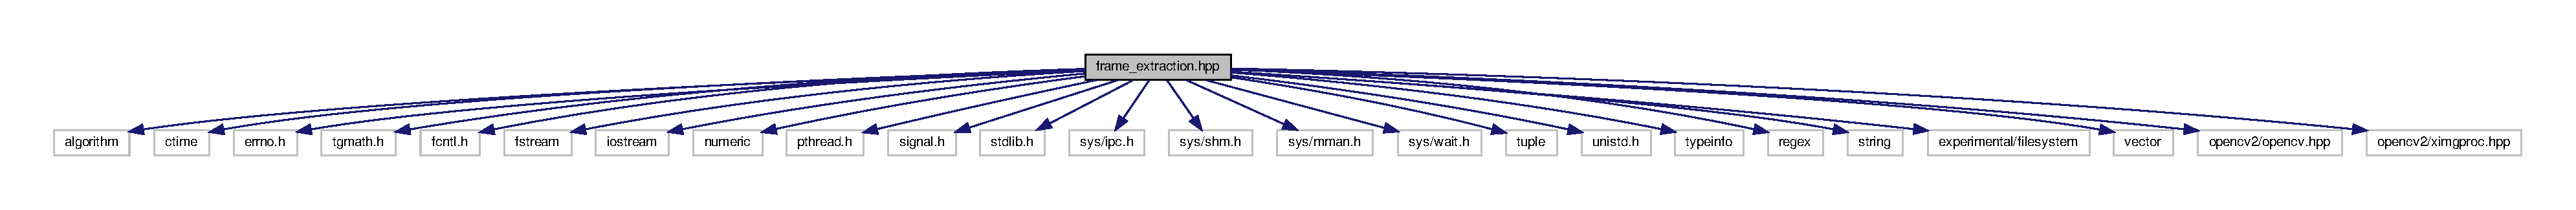
\includegraphics[width=350pt]{frame__extraction_8hpp__incl}
\end{center}
\end{figure}
This graph shows which files directly or indirectly include this file\+:\nopagebreak
\begin{figure}[H]
\begin{center}
\leavevmode
\includegraphics[width=188pt]{frame__extraction_8hpp__dep__incl}
\end{center}
\end{figure}
\subsection*{Functions}
\begin{DoxyCompactItemize}
\item 
static Mat \hyperlink{frame__extraction_8hpp_afae27f2c8807b9a09243b93d512b504c}{shift\+\_\+frame} (Mat in\+\_\+frame, int shiftx, int shifty)
\item 
static Mat \hyperlink{frame__extraction_8hpp_a19b6b938855c1060791509f406645605}{corner\+\_\+matching} (Mat in\+\_\+frame, vector$<$ Point $>$ contour, int plusx, int plusy)
\item 
static vector$<$ int $>$ \hyperlink{frame__extraction_8hpp_a5ef2b91877d44dada29b478b53744af6}{test\+\_\+edges} (Mat in\+\_\+frame, vector$<$ Point $>$ contour, int te\+\_\+ret)
\item 
static int \hyperlink{frame__extraction_8hpp_a8b5c97016e3cad4475344f33f288bed4}{min\+\_\+square\+\_\+dim} (Mat in\+\_\+frame)
\item 
static vector$<$ int $>$ \hyperlink{frame__extraction_8hpp_a3ac94b4b4ad476fbcdd1ac7bc26b1fe1}{edge\+\_\+width} (vector$<$ Point $>$ contour)
\item 
static vector$<$ int $>$ \hyperlink{frame__extraction_8hpp_a3eefea9d7b7944b3c17145bf1f42ca1f}{edge\+\_\+height} (vector$<$ Point $>$ contour)
\item 
static int \hyperlink{frame__extraction_8hpp_a6ebd493f01eb54e528da257db0a75e99}{initial\+\_\+crop} (Mat in\+\_\+frame, int framecnt)
\item 
static int \hyperlink{frame__extraction_8hpp_a032ee30a958a27cdb3d5b419953ab584}{touching\+\_\+edges} (Mat in\+\_\+frame, vector$<$ Point $>$ contour)
\item 
static Mat \hyperlink{frame__extraction_8hpp_a8f336c75968d8ab7d3aa3c5c8ff74dbb}{traditional\+\_\+centering} (Mat in\+\_\+frame, vector$<$ vector$<$ Point $>$$>$ contours, int largest, Rect box)
\item 
static int \hyperlink{frame__extraction_8hpp_a2dab519501e6a1106a8b0b2cbfd52511}{first\+\_\+frame} (Mat in\+\_\+frame, int framecnt)
\item 
static int \hyperlink{frame__extraction_8hpp_a9c4e877be5c7a5b6c78cf2e81c09759f}{halo\+\_\+noise\+\_\+and\+\_\+center} (Mat in\+\_\+frame, int framecnt)
\item 
static void \hyperlink{frame__extraction_8hpp_aade1bdfa6306f0627b8a1fe204aacfab}{signal\+\_\+callback\+\_\+handler} (int signum)
\item 
static Mat \hyperlink{frame__extraction_8hpp_a09f4cf8817c686df6a1992baf222b97a}{apply\+\_\+dynamic\+\_\+mask} (Mat in\+\_\+frame, vector$<$ vector$<$ Point $>$$>$ contours, int maskwidth)
\item 
static int \hyperlink{frame__extraction_8hpp_abc90f05608032b4730869812a513267f}{largest\+\_\+contour} (vector$<$ vector$<$ Point $>$$>$ contours)
\item 
static vector$<$ vector$<$ Point $>$ $>$ \hyperlink{frame__extraction_8hpp_a5a1b727e663ec81191fd584338c88227}{contours\+\_\+only} (Mat in\+\_\+frame)
\item 
static int \hyperlink{frame__extraction_8hpp_ab82da2f54d3288500af385f722ee691e}{box\+\_\+finder} (Mat in\+\_\+frame, bool do\+\_\+thresh)
\item 
static int \hyperlink{frame__extraction_8hpp_a3fe52ab2a13802c64a500f3b3fac618c}{box\+\_\+data} (Rect box, int framecnt)
\item 
static int \hyperlink{frame__extraction_8hpp_a5c53b5dffc43d3917a312ade756e53ee}{show\+\_\+usage} (string name)
\item 
static vector$<$ Point $>$ \hyperlink{frame__extraction_8hpp_a7564e59e35a0ba92812018e6ff847141}{qhe\+\_\+bigone} (Mat in\+\_\+frame)
\item 
static vector$<$ vector$<$ Point $>$ $>$ \hyperlink{frame__extraction_8hpp_ae9d9ad905beac19a35c93ee874a2c84c}{quiet\+\_\+halo\+\_\+elim} (vector$<$ vector$<$ Point $>$$>$ contours, vector$<$ Point $>$ bigone)
\item 
static int \hyperlink{frame__extraction_8hpp_aefb0c1bc7ceed8e1df9cb033fbc5b6a4}{tier\+\_\+one} (int cnt, Mat in\+\_\+frame, vector$<$ Point $>$ bigone)
\item 
static int \hyperlink{frame__extraction_8hpp_af68a26eb7b7f9df708af2adffc9bb826}{tier\+\_\+two} (int cnt, Mat in\+\_\+frame, vector$<$ Point $>$ bigone)
\item 
static int \hyperlink{frame__extraction_8hpp_af5e2d4f3ec9c6dba1ea50fe053228b0e}{tier\+\_\+three} (int cnt, Mat in\+\_\+frame, Mat old\+\_\+frame, vector$<$ Point $>$ bigone)
\item 
static int \hyperlink{frame__extraction_8hpp_a4045b12a555baf914c7c11f9d92f3c3f}{tier\+\_\+four} (int cnt, Mat in\+\_\+frame, Mat old\+\_\+frame, vector$<$ Point $>$ bigone)
\item 
static int \hyperlink{frame__extraction_8hpp_ae3f0a97a7bf6dcfbb91ffdbc9997841f}{parse\+\_\+checklist} (std\+::string name, std\+::string value)
\item 
static std\+::string \hyperlink{frame__extraction_8hpp_ae5b18af36c3bf024f8a2dc5c4fe4242b}{out\+\_\+frame\+\_\+gen} (int framecnt)
\item 
std\+::string \hyperlink{frame__extraction_8hpp_a6aa2b943656a2bdc7bbb9a4f9e1adcd1}{space\+\_\+space} (std\+::string instring)
\item 
static int \hyperlink{frame__extraction_8hpp_a272c8275ab7a0918c5e6c9acf9afda50}{generate\+\_\+slideshow} ()
\item 
static int \hyperlink{frame__extraction_8hpp_a579a6e5cf9846789c07a88e72ef4a7a7}{concat\+\_\+tiers} ()
\item 
static int \hyperlink{frame__extraction_8hpp_aaf7c365254fb30ce3015aded4fdf1c9d}{off\+\_\+screen\+\_\+ellipse} ()
\item 
static int \hyperlink{frame__extraction_8hpp_a34a2b5ae307c281071a717fc2d1fb0c6}{post\+\_\+processing} ()
\item 
int \hyperlink{frame__extraction_8hpp_a0ddf1224851353fc92bfbff6f499fa97}{main} (int argc, char $\ast$argv\mbox{[}$\,$\mbox{]})
\end{DoxyCompactItemize}
\subsection*{Variables}
\begin{DoxyCompactItemize}
\item 
int \hyperlink{frame__extraction_8hpp_a643246b9c7e8aae9940b95816b3ef619}{M\+A\+J\+O\+R\+\_\+\+V\+E\+R\+S\+I\+ON} = 0
\item 
int \hyperlink{frame__extraction_8hpp_abb401b86975b0d3bbe8ee218ec1dfb9e}{M\+I\+N\+O\+R\+\_\+\+V\+E\+R\+S\+I\+ON} = 3
\item 
std\+::string \hyperlink{frame__extraction_8hpp_a47b8f3b7316940a45a22887c0bbb16ff}{A\+L\+P\+H\+A\+\_\+\+B\+E\+TA} = \char`\"{}-\/alpha\char`\"{}
\item 
int \hyperlink{frame__extraction_8hpp_a4b33c72393dc53e828d8804e494eb19b}{S\+I\+G\+\_\+\+A\+L\+E\+RT} = 0
\item 
double \hyperlink{frame__extraction_8hpp_adb6bb14924c1a64069b47a1eb7cda998}{O\+R\+I\+G\+\_\+\+A\+R\+EA}
\item 
double \hyperlink{frame__extraction_8hpp_ac5f19d11a403b7ad0b79666f4a9e45be}{O\+R\+I\+G\+\_\+\+P\+E\+RI}
\item 
int \hyperlink{frame__extraction_8hpp_a4c815601b99b16edcc7a1982e70f0e9e}{O\+R\+I\+G\+\_\+\+V\+E\+RT}
\item 
int \hyperlink{frame__extraction_8hpp_a54ec76f9d069579b86e56b160a7da402}{O\+R\+I\+G\+\_\+\+H\+O\+RZ}
\item 
int \hyperlink{frame__extraction_8hpp_a1606f5f6b4b3ce7562a33541cfaa2b95}{B\+O\+X\+S\+I\+ZE}
\item 
Point \hyperlink{frame__extraction_8hpp_acb578913128994d581db4f656ec6ae00}{O\+R\+I\+G\+\_\+\+TL}
\item 
Point \hyperlink{frame__extraction_8hpp_a71965c5a7e184f68831392f8082a0db6}{O\+R\+I\+G\+\_\+\+BR}
\item 
std\+::string \hyperlink{frame__extraction_8hpp_aa44a0c0d379a7ae7b683d9154ba78049}{L\+O\+G\+O\+UT}
\item 
std\+::ofstream \hyperlink{frame__extraction_8hpp_a8a1edfd43d430d0373c6a82630d92e19}{L\+O\+G\+G\+I\+NG}
\item 
std\+::string \hyperlink{frame__extraction_8hpp_adfd48c73bc7c1ce3c8bd6cf4dc372d1b}{T\+I\+E\+R1\+F\+I\+LE}
\item 
std\+::string \hyperlink{frame__extraction_8hpp_a358c442f23ef765d997f7933db7cdee8}{T\+I\+E\+R2\+F\+I\+LE}
\item 
std\+::string \hyperlink{frame__extraction_8hpp_a5d72abb5d5323de0995523b9f9d0e4f2}{T\+I\+E\+R3\+F\+I\+LE}
\item 
std\+::string \hyperlink{frame__extraction_8hpp_a60b27aa6c536e170d7626247f25e00c0}{T\+I\+E\+R4\+F\+I\+LE}
\item 
std\+::string \hyperlink{frame__extraction_8hpp_a3490374a73148475d598efb7c402f152}{E\+L\+L\+I\+P\+S\+E\+D\+A\+TA}
\item 
std\+::string \hyperlink{frame__extraction_8hpp_a466ff90ffe29746d905f7c2c607f66dd}{B\+O\+X\+D\+A\+TA}
\item 
std\+::string \hyperlink{frame__extraction_8hpp_a0a4abfcd44b1d02d561957a51473ab87}{M\+E\+T\+A\+D\+A\+TA}
\item 
int \hyperlink{frame__extraction_8hpp_ab49dcecdf57f9a30448512927af37149}{T\+C\+\_\+W}
\item 
int \hyperlink{frame__extraction_8hpp_a1029100fd4afc96ef1203f673502a653}{T\+C\+\_\+H}
\item 
bool \hyperlink{frame__extraction_8hpp_a35bb5d6f37460d37ae05b5c0820634b0}{C\+A\+U\+G\+H\+T\+\_\+\+E\+M\+P\+TY} = false
\item 
bool \hyperlink{frame__extraction_8hpp_a10068bb1ce382c3d7de90340f52822ff}{D\+E\+B\+U\+G\+\_\+\+F\+R\+A\+M\+ES} = false
\item 
bool \hyperlink{frame__extraction_8hpp_a83dadb8aa01947b593534c053344a213}{D\+E\+B\+U\+G\+\_\+\+C\+O\+UT} = false
\item 
bool \hyperlink{frame__extraction_8hpp_aacdde62571ea0c9c4a444fb0a2e07c86}{O\+U\+T\+P\+U\+T\+\_\+\+F\+R\+A\+M\+ES} = false
\item 
bool \hyperlink{frame__extraction_8hpp_aecf9aa0f271ffbf601366d895c2c6cc8}{E\+M\+P\+T\+Y\+\_\+\+F\+R\+A\+M\+ES} = true
\item 
bool \hyperlink{frame__extraction_8hpp_a520f172801d4e425d888d5e983e2fadf}{G\+E\+N\+\_\+\+S\+L\+I\+D\+E\+S\+H\+OW} = true
\item 
bool \hyperlink{frame__extraction_8hpp_ac500b5571565b1e88603ba674fc3099e}{S\+I\+M\+P\+\_\+\+E\+LL} = true
\item 
bool \hyperlink{frame__extraction_8hpp_a8e15ce073c27310f8852293c1e63adff}{C\+O\+N\+C\+A\+T\+\_\+\+T\+I\+E\+RS} = true
\item 
bool \hyperlink{frame__extraction_8hpp_a37fe90d7f18dca0a4587be9f480bd857}{T\+I\+G\+H\+T\+\_\+\+C\+R\+OP} = true
\item 
std\+::string \hyperlink{frame__extraction_8hpp_acfbb0cca61124eb6def3b6b423ea126c}{O\+S\+F\+P\+R\+O\+J\+E\+CT} = \char`\"{}\char`\"{}
\item 
std\+::string \hyperlink{frame__extraction_8hpp_af5942e22ad18b34b76aac3198ed301a7}{O\+U\+T\+P\+U\+T\+D\+IR} = \char`\"{}Birdtracker\+\_\+\+Output/\char`\"{}
\item 
int \hyperlink{frame__extraction_8hpp_a2332079d8f52c6b83c3ad88bc07d7fc0}{E\+D\+G\+E\+T\+H\+R\+E\+SH} = 10
\item 
int \hyperlink{frame__extraction_8hpp_ab4a8b7063262f24b88b18e8fc87ef249}{Q\+H\+E\+\_\+\+W\+I\+D\+TH} = 10
\item 
int \hyperlink{frame__extraction_8hpp_a9dac10009ab7d65a666e505012a79722}{B\+L\+A\+C\+K\+O\+U\+T\+\_\+\+T\+H\+R\+E\+SH} = 51
\item 
int \hyperlink{frame__extraction_8hpp_ad146592969bbf6ece87549556561a3ff}{C\+O\+N\+V\+E\+R\+T\+\_\+\+F\+PS} = 30
\item 
int \hyperlink{frame__extraction_8hpp_a3462204ca77e6259e482b34e38a852b4}{N\+O\+N\+\_\+\+Z\+E\+R\+O\+\_\+\+S\+T\+A\+RT} = 0
\item 
int \hyperlink{frame__extraction_8hpp_aeea4b78659f16fb276d7a18056557b21}{Q\+H\+E\+\_\+\+G\+B\+\_\+\+K\+E\+R\+N\+E\+L\+\_\+X} = 15
\item 
int \hyperlink{frame__extraction_8hpp_ae528b26104cf3efbaa603349b0de72dd}{Q\+H\+E\+\_\+\+G\+B\+\_\+\+K\+E\+R\+N\+E\+L\+\_\+Y} = 15
\item 
double \hyperlink{frame__extraction_8hpp_ad7f767bdb807131c04268d9a626940d0}{Q\+H\+E\+\_\+\+G\+B\+\_\+\+S\+I\+G\+M\+A\+\_\+X} = 1
\item 
double \hyperlink{frame__extraction_8hpp_a4111a02865ed1f29b7eb2c931c67fb82}{Q\+H\+E\+\_\+\+G\+B\+\_\+\+S\+I\+G\+M\+A\+\_\+Y} = 1
\item 
double \hyperlink{frame__extraction_8hpp_a653f64d9971448710226dc272ea46d3f}{T1\+\_\+\+A\+T\+\_\+\+M\+AX} = 255
\item 
int \hyperlink{frame__extraction_8hpp_a0b965756b91cadfff1e64d0efccac874}{T1\+\_\+\+A\+T\+\_\+\+B\+L\+O\+C\+K\+S\+I\+ZE} = 65
\item 
double \hyperlink{frame__extraction_8hpp_a2cbacf3bd2938a25a3953ad5dbc2277e}{T1\+\_\+\+A\+T\+\_\+\+C\+O\+N\+S\+T\+A\+NT} = 35
\item 
int \hyperlink{frame__extraction_8hpp_a52844cd184dc85cb3e03bfd809e6ae2f}{T1\+\_\+\+D\+Y\+M\+A\+SK} = 25
\item 
double \hyperlink{frame__extraction_8hpp_a412e3790c42bd5f9501367d455b3751d}{T2\+\_\+\+A\+T\+\_\+\+M\+AX} = 255
\item 
int \hyperlink{frame__extraction_8hpp_a0587125db3966d21910b315b8891c42e}{T2\+\_\+\+A\+T\+\_\+\+B\+L\+O\+C\+K\+S\+I\+ZE} = 65
\item 
double \hyperlink{frame__extraction_8hpp_a5b70ffbccfd7d4b80c32a46be6858b7e}{T2\+\_\+\+A\+T\+\_\+\+C\+O\+N\+S\+T\+A\+NT} = 20
\item 
int \hyperlink{frame__extraction_8hpp_a2b81ffcb17284477cc35f0076629498f}{T2\+\_\+\+D\+Y\+M\+A\+SK} = 25
\item 
int \hyperlink{frame__extraction_8hpp_ac14a005bb9acc6aa5545bf39af2fa9ee}{T3\+\_\+\+L\+A\+P\+\_\+\+K\+E\+R\+N\+EL} = 11
\item 
double \hyperlink{frame__extraction_8hpp_aa55164dad8d87e7b78a9bd55ad7d1c45}{T3\+\_\+\+L\+A\+P\+\_\+\+S\+C\+A\+LE} = 0.\+0001
\item 
double \hyperlink{frame__extraction_8hpp_a4f9e67146723dce813577779d4eea9e1}{T3\+\_\+\+L\+A\+P\+\_\+\+D\+E\+L\+TA} = 0
\item 
int \hyperlink{frame__extraction_8hpp_ad89c57b77d7bd6d372dc98ce22cbb6d7}{T3\+\_\+\+G\+B\+\_\+\+K\+E\+R\+N\+E\+L\+\_\+X} = 11
\item 
int \hyperlink{frame__extraction_8hpp_afad19635c436b356711b63b7069d2357}{T3\+\_\+\+G\+B\+\_\+\+K\+E\+R\+N\+E\+L\+\_\+Y} = 11
\item 
double \hyperlink{frame__extraction_8hpp_ab2745a0941d78b709a9dd15b2af6755b}{T3\+\_\+\+G\+B\+\_\+\+S\+I\+G\+M\+A\+\_\+X} = 1
\item 
double \hyperlink{frame__extraction_8hpp_ae5d0636e04fbd69319bf21f04f1cb0ef}{T3\+\_\+\+G\+B\+\_\+\+S\+I\+G\+M\+A\+\_\+Y} = 1
\item 
int \hyperlink{frame__extraction_8hpp_ac466f080a5d1bfa01cdd96d81b2cb294}{T3\+\_\+\+C\+U\+T\+O\+F\+F\+\_\+\+T\+H\+R\+E\+SH} = 40
\item 
int \hyperlink{frame__extraction_8hpp_ad4873501452b2bf72f6db4c494bc6443}{T3\+\_\+\+D\+Y\+M\+A\+SK} = 45
\item 
double \hyperlink{frame__extraction_8hpp_abc16bb52e9f98041a153f5f4b45e0620}{T4\+\_\+\+A\+T\+\_\+\+M\+AX} = 255
\item 
int \hyperlink{frame__extraction_8hpp_a78e73af530570d6b16032c02595e48f8}{T4\+\_\+\+A\+T\+\_\+\+B\+L\+O\+C\+K\+S\+I\+ZE} = 65
\item 
double \hyperlink{frame__extraction_8hpp_a88fc5916ea23147161871a9085e763f4}{T4\+\_\+\+A\+T\+\_\+\+C\+O\+N\+S\+T\+A\+NT} = 20
\item 
double \hyperlink{frame__extraction_8hpp_abf615655f0218dcda240084c9962cbfd}{T4\+\_\+\+P\+O\+W\+ER} = 2
\item 
int \hyperlink{frame__extraction_8hpp_a2dd46160d3cb5810e1cd60dd1fcd82e5}{T4\+\_\+\+G\+B\+\_\+\+K\+E\+R\+N\+E\+L\+\_\+X} = 11
\item 
int \hyperlink{frame__extraction_8hpp_aee35e4eb8ecc472a59cd20946c5cc387}{T4\+\_\+\+G\+B\+\_\+\+K\+E\+R\+N\+E\+L\+\_\+Y} = 11
\item 
double \hyperlink{frame__extraction_8hpp_a1e7d063ef3731c780479690071535f5b}{T4\+\_\+\+G\+B\+\_\+\+S\+I\+G\+M\+A\+\_\+X} = 1
\item 
double \hyperlink{frame__extraction_8hpp_acf6f7063280f25a04a975396f48d0910}{T4\+\_\+\+G\+B\+\_\+\+S\+I\+G\+M\+A\+\_\+Y} = 1
\item 
int \hyperlink{frame__extraction_8hpp_a51c1de4947ef778b0fd580b7b7c1d3e9}{T4\+\_\+\+T\+H\+I\+N\+N\+I\+NG} = 0
\item 
int \hyperlink{frame__extraction_8hpp_a25e7cae5e0555d85c848342cfa92686c}{T4\+\_\+\+D\+Y\+M\+A\+SK} = 45
\end{DoxyCompactItemize}


\subsection{Function Documentation}
\mbox{\Hypertarget{frame__extraction_8hpp_a09f4cf8817c686df6a1992baf222b97a}\label{frame__extraction_8hpp_a09f4cf8817c686df6a1992baf222b97a}} 
\index{frame\+\_\+extraction.\+hpp@{frame\+\_\+extraction.\+hpp}!apply\+\_\+dynamic\+\_\+mask@{apply\+\_\+dynamic\+\_\+mask}}
\index{apply\+\_\+dynamic\+\_\+mask@{apply\+\_\+dynamic\+\_\+mask}!frame\+\_\+extraction.\+hpp@{frame\+\_\+extraction.\+hpp}}
\subsubsection{\texorpdfstring{apply\+\_\+dynamic\+\_\+mask()}{apply\_dynamic\_mask()}}
{\footnotesize\ttfamily static Mat apply\+\_\+dynamic\+\_\+mask (\begin{DoxyParamCaption}\item[{Mat}]{in\+\_\+frame,  }\item[{vector$<$ vector$<$ Point $>$$>$}]{contours,  }\item[{int}]{maskwidth }\end{DoxyParamCaption})\hspace{0.3cm}{\ttfamily [static]}}

\mbox{\Hypertarget{frame__extraction_8hpp_a3fe52ab2a13802c64a500f3b3fac618c}\label{frame__extraction_8hpp_a3fe52ab2a13802c64a500f3b3fac618c}} 
\index{frame\+\_\+extraction.\+hpp@{frame\+\_\+extraction.\+hpp}!box\+\_\+data@{box\+\_\+data}}
\index{box\+\_\+data@{box\+\_\+data}!frame\+\_\+extraction.\+hpp@{frame\+\_\+extraction.\+hpp}}
\subsubsection{\texorpdfstring{box\+\_\+data()}{box\_data()}}
{\footnotesize\ttfamily static int box\+\_\+data (\begin{DoxyParamCaption}\item[{Rect}]{box,  }\item[{int}]{framecnt }\end{DoxyParamCaption})\hspace{0.3cm}{\ttfamily [static]}}

\mbox{\Hypertarget{frame__extraction_8hpp_ab82da2f54d3288500af385f722ee691e}\label{frame__extraction_8hpp_ab82da2f54d3288500af385f722ee691e}} 
\index{frame\+\_\+extraction.\+hpp@{frame\+\_\+extraction.\+hpp}!box\+\_\+finder@{box\+\_\+finder}}
\index{box\+\_\+finder@{box\+\_\+finder}!frame\+\_\+extraction.\+hpp@{frame\+\_\+extraction.\+hpp}}
\subsubsection{\texorpdfstring{box\+\_\+finder()}{box\_finder()}}
{\footnotesize\ttfamily static int box\+\_\+finder (\begin{DoxyParamCaption}\item[{Mat}]{in\+\_\+frame,  }\item[{bool}]{do\+\_\+thresh }\end{DoxyParamCaption})\hspace{0.3cm}{\ttfamily [static]}}

\mbox{\Hypertarget{frame__extraction_8hpp_a579a6e5cf9846789c07a88e72ef4a7a7}\label{frame__extraction_8hpp_a579a6e5cf9846789c07a88e72ef4a7a7}} 
\index{frame\+\_\+extraction.\+hpp@{frame\+\_\+extraction.\+hpp}!concat\+\_\+tiers@{concat\+\_\+tiers}}
\index{concat\+\_\+tiers@{concat\+\_\+tiers}!frame\+\_\+extraction.\+hpp@{frame\+\_\+extraction.\+hpp}}
\subsubsection{\texorpdfstring{concat\+\_\+tiers()}{concat\_tiers()}}
{\footnotesize\ttfamily static int concat\+\_\+tiers (\begin{DoxyParamCaption}{ }\end{DoxyParamCaption})\hspace{0.3cm}{\ttfamily [static]}}

\mbox{\Hypertarget{frame__extraction_8hpp_a5a1b727e663ec81191fd584338c88227}\label{frame__extraction_8hpp_a5a1b727e663ec81191fd584338c88227}} 
\index{frame\+\_\+extraction.\+hpp@{frame\+\_\+extraction.\+hpp}!contours\+\_\+only@{contours\+\_\+only}}
\index{contours\+\_\+only@{contours\+\_\+only}!frame\+\_\+extraction.\+hpp@{frame\+\_\+extraction.\+hpp}}
\subsubsection{\texorpdfstring{contours\+\_\+only()}{contours\_only()}}
{\footnotesize\ttfamily static vector$<$vector$<$Point$>$ $>$ contours\+\_\+only (\begin{DoxyParamCaption}\item[{Mat}]{in\+\_\+frame }\end{DoxyParamCaption})\hspace{0.3cm}{\ttfamily [static]}}

\mbox{\Hypertarget{frame__extraction_8hpp_a19b6b938855c1060791509f406645605}\label{frame__extraction_8hpp_a19b6b938855c1060791509f406645605}} 
\index{frame\+\_\+extraction.\+hpp@{frame\+\_\+extraction.\+hpp}!corner\+\_\+matching@{corner\+\_\+matching}}
\index{corner\+\_\+matching@{corner\+\_\+matching}!frame\+\_\+extraction.\+hpp@{frame\+\_\+extraction.\+hpp}}
\subsubsection{\texorpdfstring{corner\+\_\+matching()}{corner\_matching()}}
{\footnotesize\ttfamily static Mat corner\+\_\+matching (\begin{DoxyParamCaption}\item[{Mat}]{in\+\_\+frame,  }\item[{vector$<$ Point $>$}]{contour,  }\item[{int}]{plusx,  }\item[{int}]{plusy }\end{DoxyParamCaption})\hspace{0.3cm}{\ttfamily [static]}}

\mbox{\Hypertarget{frame__extraction_8hpp_a3eefea9d7b7944b3c17145bf1f42ca1f}\label{frame__extraction_8hpp_a3eefea9d7b7944b3c17145bf1f42ca1f}} 
\index{frame\+\_\+extraction.\+hpp@{frame\+\_\+extraction.\+hpp}!edge\+\_\+height@{edge\+\_\+height}}
\index{edge\+\_\+height@{edge\+\_\+height}!frame\+\_\+extraction.\+hpp@{frame\+\_\+extraction.\+hpp}}
\subsubsection{\texorpdfstring{edge\+\_\+height()}{edge\_height()}}
{\footnotesize\ttfamily static vector$<$int$>$ edge\+\_\+height (\begin{DoxyParamCaption}\item[{vector$<$ Point $>$}]{contour }\end{DoxyParamCaption})\hspace{0.3cm}{\ttfamily [static]}}

\mbox{\Hypertarget{frame__extraction_8hpp_a3ac94b4b4ad476fbcdd1ac7bc26b1fe1}\label{frame__extraction_8hpp_a3ac94b4b4ad476fbcdd1ac7bc26b1fe1}} 
\index{frame\+\_\+extraction.\+hpp@{frame\+\_\+extraction.\+hpp}!edge\+\_\+width@{edge\+\_\+width}}
\index{edge\+\_\+width@{edge\+\_\+width}!frame\+\_\+extraction.\+hpp@{frame\+\_\+extraction.\+hpp}}
\subsubsection{\texorpdfstring{edge\+\_\+width()}{edge\_width()}}
{\footnotesize\ttfamily static vector$<$int$>$ edge\+\_\+width (\begin{DoxyParamCaption}\item[{vector$<$ Point $>$}]{contour }\end{DoxyParamCaption})\hspace{0.3cm}{\ttfamily [static]}}

\mbox{\Hypertarget{frame__extraction_8hpp_a2dab519501e6a1106a8b0b2cbfd52511}\label{frame__extraction_8hpp_a2dab519501e6a1106a8b0b2cbfd52511}} 
\index{frame\+\_\+extraction.\+hpp@{frame\+\_\+extraction.\+hpp}!first\+\_\+frame@{first\+\_\+frame}}
\index{first\+\_\+frame@{first\+\_\+frame}!frame\+\_\+extraction.\+hpp@{frame\+\_\+extraction.\+hpp}}
\subsubsection{\texorpdfstring{first\+\_\+frame()}{first\_frame()}}
{\footnotesize\ttfamily static int first\+\_\+frame (\begin{DoxyParamCaption}\item[{Mat}]{in\+\_\+frame,  }\item[{int}]{framecnt }\end{DoxyParamCaption})\hspace{0.3cm}{\ttfamily [static]}}

\mbox{\Hypertarget{frame__extraction_8hpp_a272c8275ab7a0918c5e6c9acf9afda50}\label{frame__extraction_8hpp_a272c8275ab7a0918c5e6c9acf9afda50}} 
\index{frame\+\_\+extraction.\+hpp@{frame\+\_\+extraction.\+hpp}!generate\+\_\+slideshow@{generate\+\_\+slideshow}}
\index{generate\+\_\+slideshow@{generate\+\_\+slideshow}!frame\+\_\+extraction.\+hpp@{frame\+\_\+extraction.\+hpp}}
\subsubsection{\texorpdfstring{generate\+\_\+slideshow()}{generate\_slideshow()}}
{\footnotesize\ttfamily static int generate\+\_\+slideshow (\begin{DoxyParamCaption}{ }\end{DoxyParamCaption})\hspace{0.3cm}{\ttfamily [static]}}

\mbox{\Hypertarget{frame__extraction_8hpp_a9c4e877be5c7a5b6c78cf2e81c09759f}\label{frame__extraction_8hpp_a9c4e877be5c7a5b6c78cf2e81c09759f}} 
\index{frame\+\_\+extraction.\+hpp@{frame\+\_\+extraction.\+hpp}!halo\+\_\+noise\+\_\+and\+\_\+center@{halo\+\_\+noise\+\_\+and\+\_\+center}}
\index{halo\+\_\+noise\+\_\+and\+\_\+center@{halo\+\_\+noise\+\_\+and\+\_\+center}!frame\+\_\+extraction.\+hpp@{frame\+\_\+extraction.\+hpp}}
\subsubsection{\texorpdfstring{halo\+\_\+noise\+\_\+and\+\_\+center()}{halo\_noise\_and\_center()}}
{\footnotesize\ttfamily static int halo\+\_\+noise\+\_\+and\+\_\+center (\begin{DoxyParamCaption}\item[{Mat}]{in\+\_\+frame,  }\item[{int}]{framecnt }\end{DoxyParamCaption})\hspace{0.3cm}{\ttfamily [static]}}

\mbox{\Hypertarget{frame__extraction_8hpp_a6ebd493f01eb54e528da257db0a75e99}\label{frame__extraction_8hpp_a6ebd493f01eb54e528da257db0a75e99}} 
\index{frame\+\_\+extraction.\+hpp@{frame\+\_\+extraction.\+hpp}!initial\+\_\+crop@{initial\+\_\+crop}}
\index{initial\+\_\+crop@{initial\+\_\+crop}!frame\+\_\+extraction.\+hpp@{frame\+\_\+extraction.\+hpp}}
\subsubsection{\texorpdfstring{initial\+\_\+crop()}{initial\_crop()}}
{\footnotesize\ttfamily static int initial\+\_\+crop (\begin{DoxyParamCaption}\item[{Mat}]{in\+\_\+frame,  }\item[{int}]{framecnt }\end{DoxyParamCaption})\hspace{0.3cm}{\ttfamily [static]}}

\mbox{\Hypertarget{frame__extraction_8hpp_abc90f05608032b4730869812a513267f}\label{frame__extraction_8hpp_abc90f05608032b4730869812a513267f}} 
\index{frame\+\_\+extraction.\+hpp@{frame\+\_\+extraction.\+hpp}!largest\+\_\+contour@{largest\+\_\+contour}}
\index{largest\+\_\+contour@{largest\+\_\+contour}!frame\+\_\+extraction.\+hpp@{frame\+\_\+extraction.\+hpp}}
\subsubsection{\texorpdfstring{largest\+\_\+contour()}{largest\_contour()}}
{\footnotesize\ttfamily static int largest\+\_\+contour (\begin{DoxyParamCaption}\item[{vector$<$ vector$<$ Point $>$$>$}]{contours }\end{DoxyParamCaption})\hspace{0.3cm}{\ttfamily [static]}}

\mbox{\Hypertarget{frame__extraction_8hpp_a0ddf1224851353fc92bfbff6f499fa97}\label{frame__extraction_8hpp_a0ddf1224851353fc92bfbff6f499fa97}} 
\index{frame\+\_\+extraction.\+hpp@{frame\+\_\+extraction.\+hpp}!main@{main}}
\index{main@{main}!frame\+\_\+extraction.\+hpp@{frame\+\_\+extraction.\+hpp}}
\subsubsection{\texorpdfstring{main()}{main()}}
{\footnotesize\ttfamily int main (\begin{DoxyParamCaption}\item[{int}]{argc,  }\item[{char $\ast$}]{argv\mbox{[}$\,$\mbox{]} }\end{DoxyParamCaption})}

Main loop


\begin{DoxyParams}{Parameters}
{\em argc} & number of input arguments \\
\hline
{\em argv} & contents of input arguments \\
\hline
\end{DoxyParams}
\begin{DoxyReturn}{Returns}
status 
\end{DoxyReturn}
Here is the call graph for this function\+:\nopagebreak
\begin{figure}[H]
\begin{center}
\leavevmode
\includegraphics[width=350pt]{frame__extraction_8hpp_a0ddf1224851353fc92bfbff6f499fa97_cgraph}
\end{center}
\end{figure}
\mbox{\Hypertarget{frame__extraction_8hpp_a8b5c97016e3cad4475344f33f288bed4}\label{frame__extraction_8hpp_a8b5c97016e3cad4475344f33f288bed4}} 
\index{frame\+\_\+extraction.\+hpp@{frame\+\_\+extraction.\+hpp}!min\+\_\+square\+\_\+dim@{min\+\_\+square\+\_\+dim}}
\index{min\+\_\+square\+\_\+dim@{min\+\_\+square\+\_\+dim}!frame\+\_\+extraction.\+hpp@{frame\+\_\+extraction.\+hpp}}
\subsubsection{\texorpdfstring{min\+\_\+square\+\_\+dim()}{min\_square\_dim()}}
{\footnotesize\ttfamily static int min\+\_\+square\+\_\+dim (\begin{DoxyParamCaption}\item[{Mat}]{in\+\_\+frame }\end{DoxyParamCaption})\hspace{0.3cm}{\ttfamily [static]}}

\mbox{\Hypertarget{frame__extraction_8hpp_aaf7c365254fb30ce3015aded4fdf1c9d}\label{frame__extraction_8hpp_aaf7c365254fb30ce3015aded4fdf1c9d}} 
\index{frame\+\_\+extraction.\+hpp@{frame\+\_\+extraction.\+hpp}!off\+\_\+screen\+\_\+ellipse@{off\+\_\+screen\+\_\+ellipse}}
\index{off\+\_\+screen\+\_\+ellipse@{off\+\_\+screen\+\_\+ellipse}!frame\+\_\+extraction.\+hpp@{frame\+\_\+extraction.\+hpp}}
\subsubsection{\texorpdfstring{off\+\_\+screen\+\_\+ellipse()}{off\_screen\_ellipse()}}
{\footnotesize\ttfamily static int off\+\_\+screen\+\_\+ellipse (\begin{DoxyParamCaption}{ }\end{DoxyParamCaption})\hspace{0.3cm}{\ttfamily [static]}}

\mbox{\Hypertarget{frame__extraction_8hpp_ae5b18af36c3bf024f8a2dc5c4fe4242b}\label{frame__extraction_8hpp_ae5b18af36c3bf024f8a2dc5c4fe4242b}} 
\index{frame\+\_\+extraction.\+hpp@{frame\+\_\+extraction.\+hpp}!out\+\_\+frame\+\_\+gen@{out\+\_\+frame\+\_\+gen}}
\index{out\+\_\+frame\+\_\+gen@{out\+\_\+frame\+\_\+gen}!frame\+\_\+extraction.\+hpp@{frame\+\_\+extraction.\+hpp}}
\subsubsection{\texorpdfstring{out\+\_\+frame\+\_\+gen()}{out\_frame\_gen()}}
{\footnotesize\ttfamily static std\+::string out\+\_\+frame\+\_\+gen (\begin{DoxyParamCaption}\item[{int}]{framecnt }\end{DoxyParamCaption})\hspace{0.3cm}{\ttfamily [static]}}

\mbox{\Hypertarget{frame__extraction_8hpp_ae3f0a97a7bf6dcfbb91ffdbc9997841f}\label{frame__extraction_8hpp_ae3f0a97a7bf6dcfbb91ffdbc9997841f}} 
\index{frame\+\_\+extraction.\+hpp@{frame\+\_\+extraction.\+hpp}!parse\+\_\+checklist@{parse\+\_\+checklist}}
\index{parse\+\_\+checklist@{parse\+\_\+checklist}!frame\+\_\+extraction.\+hpp@{frame\+\_\+extraction.\+hpp}}
\subsubsection{\texorpdfstring{parse\+\_\+checklist()}{parse\_checklist()}}
{\footnotesize\ttfamily static int parse\+\_\+checklist (\begin{DoxyParamCaption}\item[{std\+::string}]{name,  }\item[{std\+::string}]{value }\end{DoxyParamCaption})\hspace{0.3cm}{\ttfamily [static]}}

This function handles the strings and values parsed from the settings.\+cfg file and assigns them to the global values.


\begin{DoxyParams}{Parameters}
{\em name} & String obtained while parsing the settings.\+cfg file \\
\hline
{\em value} & The value associated with name from settings.\+cfg file \\
\hline
\end{DoxyParams}
\begin{DoxyReturn}{Returns}
status 
\end{DoxyReturn}
Here is the caller graph for this function\+:\nopagebreak
\begin{figure}[H]
\begin{center}
\leavevmode
\includegraphics[width=239pt]{frame__extraction_8hpp_ae3f0a97a7bf6dcfbb91ffdbc9997841f_icgraph}
\end{center}
\end{figure}
\mbox{\Hypertarget{frame__extraction_8hpp_a34a2b5ae307c281071a717fc2d1fb0c6}\label{frame__extraction_8hpp_a34a2b5ae307c281071a717fc2d1fb0c6}} 
\index{frame\+\_\+extraction.\+hpp@{frame\+\_\+extraction.\+hpp}!post\+\_\+processing@{post\+\_\+processing}}
\index{post\+\_\+processing@{post\+\_\+processing}!frame\+\_\+extraction.\+hpp@{frame\+\_\+extraction.\+hpp}}
\subsubsection{\texorpdfstring{post\+\_\+processing()}{post\_processing()}}
{\footnotesize\ttfamily static int post\+\_\+processing (\begin{DoxyParamCaption}{ }\end{DoxyParamCaption})\hspace{0.3cm}{\ttfamily [static]}}

\mbox{\Hypertarget{frame__extraction_8hpp_a7564e59e35a0ba92812018e6ff847141}\label{frame__extraction_8hpp_a7564e59e35a0ba92812018e6ff847141}} 
\index{frame\+\_\+extraction.\+hpp@{frame\+\_\+extraction.\+hpp}!qhe\+\_\+bigone@{qhe\+\_\+bigone}}
\index{qhe\+\_\+bigone@{qhe\+\_\+bigone}!frame\+\_\+extraction.\+hpp@{frame\+\_\+extraction.\+hpp}}
\subsubsection{\texorpdfstring{qhe\+\_\+bigone()}{qhe\_bigone()}}
{\footnotesize\ttfamily static vector$<$Point$>$ qhe\+\_\+bigone (\begin{DoxyParamCaption}\item[{Mat}]{in\+\_\+frame }\end{DoxyParamCaption})\hspace{0.3cm}{\ttfamily [static]}}

\mbox{\Hypertarget{frame__extraction_8hpp_ae9d9ad905beac19a35c93ee874a2c84c}\label{frame__extraction_8hpp_ae9d9ad905beac19a35c93ee874a2c84c}} 
\index{frame\+\_\+extraction.\+hpp@{frame\+\_\+extraction.\+hpp}!quiet\+\_\+halo\+\_\+elim@{quiet\+\_\+halo\+\_\+elim}}
\index{quiet\+\_\+halo\+\_\+elim@{quiet\+\_\+halo\+\_\+elim}!frame\+\_\+extraction.\+hpp@{frame\+\_\+extraction.\+hpp}}
\subsubsection{\texorpdfstring{quiet\+\_\+halo\+\_\+elim()}{quiet\_halo\_elim()}}
{\footnotesize\ttfamily static vector$<$vector$<$Point$>$ $>$ quiet\+\_\+halo\+\_\+elim (\begin{DoxyParamCaption}\item[{vector$<$ vector$<$ Point $>$$>$}]{contours,  }\item[{vector$<$ Point $>$}]{bigone }\end{DoxyParamCaption})\hspace{0.3cm}{\ttfamily [static]}}

\mbox{\Hypertarget{frame__extraction_8hpp_afae27f2c8807b9a09243b93d512b504c}\label{frame__extraction_8hpp_afae27f2c8807b9a09243b93d512b504c}} 
\index{frame\+\_\+extraction.\+hpp@{frame\+\_\+extraction.\+hpp}!shift\+\_\+frame@{shift\+\_\+frame}}
\index{shift\+\_\+frame@{shift\+\_\+frame}!frame\+\_\+extraction.\+hpp@{frame\+\_\+extraction.\+hpp}}
\subsubsection{\texorpdfstring{shift\+\_\+frame()}{shift\_frame()}}
{\footnotesize\ttfamily static Mat shift\+\_\+frame (\begin{DoxyParamCaption}\item[{Mat}]{in\+\_\+frame,  }\item[{int}]{shiftx,  }\item[{int}]{shifty }\end{DoxyParamCaption})\hspace{0.3cm}{\ttfamily [static]}}

\mbox{\Hypertarget{frame__extraction_8hpp_a5c53b5dffc43d3917a312ade756e53ee}\label{frame__extraction_8hpp_a5c53b5dffc43d3917a312ade756e53ee}} 
\index{frame\+\_\+extraction.\+hpp@{frame\+\_\+extraction.\+hpp}!show\+\_\+usage@{show\+\_\+usage}}
\index{show\+\_\+usage@{show\+\_\+usage}!frame\+\_\+extraction.\+hpp@{frame\+\_\+extraction.\+hpp}}
\subsubsection{\texorpdfstring{show\+\_\+usage()}{show\_usage()}}
{\footnotesize\ttfamily static int show\+\_\+usage (\begin{DoxyParamCaption}\item[{string}]{name }\end{DoxyParamCaption})\hspace{0.3cm}{\ttfamily [static]}}

\mbox{\Hypertarget{frame__extraction_8hpp_aade1bdfa6306f0627b8a1fe204aacfab}\label{frame__extraction_8hpp_aade1bdfa6306f0627b8a1fe204aacfab}} 
\index{frame\+\_\+extraction.\+hpp@{frame\+\_\+extraction.\+hpp}!signal\+\_\+callback\+\_\+handler@{signal\+\_\+callback\+\_\+handler}}
\index{signal\+\_\+callback\+\_\+handler@{signal\+\_\+callback\+\_\+handler}!frame\+\_\+extraction.\+hpp@{frame\+\_\+extraction.\+hpp}}
\subsubsection{\texorpdfstring{signal\+\_\+callback\+\_\+handler()}{signal\_callback\_handler()}}
{\footnotesize\ttfamily static void signal\+\_\+callback\+\_\+handler (\begin{DoxyParamCaption}\item[{int}]{signum }\end{DoxyParamCaption})\hspace{0.3cm}{\ttfamily [static]}}

This is a helper function to handle terminal signals. This shuts down the various forks properly when an interrupt is caught.


\begin{DoxyParams}{Parameters}
{\em signum} & signal number passed to this function. Only handles 2. \\
\hline
\end{DoxyParams}
Here is the caller graph for this function\+:\nopagebreak
\begin{figure}[H]
\begin{center}
\leavevmode
\includegraphics[width=274pt]{frame__extraction_8hpp_aade1bdfa6306f0627b8a1fe204aacfab_icgraph}
\end{center}
\end{figure}
\mbox{\Hypertarget{frame__extraction_8hpp_a6aa2b943656a2bdc7bbb9a4f9e1adcd1}\label{frame__extraction_8hpp_a6aa2b943656a2bdc7bbb9a4f9e1adcd1}} 
\index{frame\+\_\+extraction.\+hpp@{frame\+\_\+extraction.\+hpp}!space\+\_\+space@{space\+\_\+space}}
\index{space\+\_\+space@{space\+\_\+space}!frame\+\_\+extraction.\+hpp@{frame\+\_\+extraction.\+hpp}}
\subsubsection{\texorpdfstring{space\+\_\+space()}{space\_space()}}
{\footnotesize\ttfamily std\+::string space\+\_\+space (\begin{DoxyParamCaption}\item[{std\+::string}]{instring }\end{DoxyParamCaption})}

This helper function handles spaces in user paths.


\begin{DoxyParams}{Parameters}
{\em instring} & the input string \\
\hline
\end{DoxyParams}
\begin{DoxyReturn}{Returns}
outstring the corrected string 
\end{DoxyReturn}
Here is the caller graph for this function\+:\nopagebreak
\begin{figure}[H]
\begin{center}
\leavevmode
\includegraphics[width=350pt]{frame__extraction_8hpp_a6aa2b943656a2bdc7bbb9a4f9e1adcd1_icgraph}
\end{center}
\end{figure}
\mbox{\Hypertarget{frame__extraction_8hpp_a5ef2b91877d44dada29b478b53744af6}\label{frame__extraction_8hpp_a5ef2b91877d44dada29b478b53744af6}} 
\index{frame\+\_\+extraction.\+hpp@{frame\+\_\+extraction.\+hpp}!test\+\_\+edges@{test\+\_\+edges}}
\index{test\+\_\+edges@{test\+\_\+edges}!frame\+\_\+extraction.\+hpp@{frame\+\_\+extraction.\+hpp}}
\subsubsection{\texorpdfstring{test\+\_\+edges()}{test\_edges()}}
{\footnotesize\ttfamily static vector$<$int$>$ test\+\_\+edges (\begin{DoxyParamCaption}\item[{Mat}]{in\+\_\+frame,  }\item[{vector$<$ Point $>$}]{contour,  }\item[{int}]{te\+\_\+ret }\end{DoxyParamCaption})\hspace{0.3cm}{\ttfamily [static]}}

\mbox{\Hypertarget{frame__extraction_8hpp_a4045b12a555baf914c7c11f9d92f3c3f}\label{frame__extraction_8hpp_a4045b12a555baf914c7c11f9d92f3c3f}} 
\index{frame\+\_\+extraction.\+hpp@{frame\+\_\+extraction.\+hpp}!tier\+\_\+four@{tier\+\_\+four}}
\index{tier\+\_\+four@{tier\+\_\+four}!frame\+\_\+extraction.\+hpp@{frame\+\_\+extraction.\+hpp}}
\subsubsection{\texorpdfstring{tier\+\_\+four()}{tier\_four()}}
{\footnotesize\ttfamily static int tier\+\_\+four (\begin{DoxyParamCaption}\item[{int}]{framecnt,  }\item[{Mat}]{in\+\_\+frame,  }\item[{Mat}]{old\+\_\+frame,  }\item[{vector$<$ Point $>$}]{bigone }\end{DoxyParamCaption})\hspace{0.3cm}{\ttfamily [static]}}

This is the fourth pass to detect valid contours in a frame. The parameters of the function are set in the T4 section of settings.\+cfg. This is the Un\+Canny method for detecting motion. The steps are essentially the backward operation of the steps taken during Canny filtering. The current frame is subtracted from the previous frame, and this output is threholded. The thresholded image is then passed through directional Sobel filters to separate the x and y components. These components are squared, added to each other, and square rooted. The output is rescaled to match the input value ranges, and a Gaussian blur is applied. Since this output is messy, the blurry image is processed using Zhang-\/\+Suen thinning to get distinct edges. Any details lost between the blurring and thinning steps reduce noise. Contours are then detected in the normal way.


\begin{DoxyParams}{Parameters}
{\em framecnt} & int of nth frame retrieved by program \\
\hline
{\em in\+\_\+frame} & Open\+CV matrix image, 16-\/bit single depth format \\
\hline
{\em old\+\_\+frame} & Open\+CV matrix image, 16-\/bit single depth format, stored from previous cycle \\
\hline
{\em bigone} & vector of Opencv Points representing the largest contour from qhe\+\_\+bigone \\
\hline
\end{DoxyParams}
\begin{DoxyReturn}{Returns}
status 
\end{DoxyReturn}
Here is the call graph for this function\+:\nopagebreak
\begin{figure}[H]
\begin{center}
\leavevmode
\includegraphics[width=279pt]{frame__extraction_8hpp_a4045b12a555baf914c7c11f9d92f3c3f_cgraph}
\end{center}
\end{figure}
Here is the caller graph for this function\+:\nopagebreak
\begin{figure}[H]
\begin{center}
\leavevmode
\includegraphics[width=206pt]{frame__extraction_8hpp_a4045b12a555baf914c7c11f9d92f3c3f_icgraph}
\end{center}
\end{figure}
\mbox{\Hypertarget{frame__extraction_8hpp_aefb0c1bc7ceed8e1df9cb033fbc5b6a4}\label{frame__extraction_8hpp_aefb0c1bc7ceed8e1df9cb033fbc5b6a4}} 
\index{frame\+\_\+extraction.\+hpp@{frame\+\_\+extraction.\+hpp}!tier\+\_\+one@{tier\+\_\+one}}
\index{tier\+\_\+one@{tier\+\_\+one}!frame\+\_\+extraction.\+hpp@{frame\+\_\+extraction.\+hpp}}
\subsubsection{\texorpdfstring{tier\+\_\+one()}{tier\_one()}}
{\footnotesize\ttfamily static int tier\+\_\+one (\begin{DoxyParamCaption}\item[{int}]{framecnt,  }\item[{Mat}]{in\+\_\+frame,  }\item[{vector$<$ Point $>$}]{bigone }\end{DoxyParamCaption})\hspace{0.3cm}{\ttfamily [static]}}

This is the first pass to detect valid contours in a frame. The parameters of the function are set in the T1 section of settings.\+cfg. Contours are detected based on a relatively strict Open\+CV adaptive\+Threshold function. These should be gauranteed \char`\"{}hits\char`\"{}.


\begin{DoxyParams}{Parameters}
{\em framecnt} & int of nth frame retrieved by program \\
\hline
{\em in\+\_\+frame} & Open\+CV matrix image, 16-\/bit single depth format \\
\hline
{\em bigone} & vector of Opencv Points representing the largest contour from qhe\+\_\+bigone \\
\hline
\end{DoxyParams}
\begin{DoxyReturn}{Returns}
status 
\end{DoxyReturn}
Here is the call graph for this function\+:\nopagebreak
\begin{figure}[H]
\begin{center}
\leavevmode
\includegraphics[width=278pt]{frame__extraction_8hpp_aefb0c1bc7ceed8e1df9cb033fbc5b6a4_cgraph}
\end{center}
\end{figure}
Here is the caller graph for this function\+:\nopagebreak
\begin{figure}[H]
\begin{center}
\leavevmode
\includegraphics[width=205pt]{frame__extraction_8hpp_aefb0c1bc7ceed8e1df9cb033fbc5b6a4_icgraph}
\end{center}
\end{figure}
\mbox{\Hypertarget{frame__extraction_8hpp_af5e2d4f3ec9c6dba1ea50fe053228b0e}\label{frame__extraction_8hpp_af5e2d4f3ec9c6dba1ea50fe053228b0e}} 
\index{frame\+\_\+extraction.\+hpp@{frame\+\_\+extraction.\+hpp}!tier\+\_\+three@{tier\+\_\+three}}
\index{tier\+\_\+three@{tier\+\_\+three}!frame\+\_\+extraction.\+hpp@{frame\+\_\+extraction.\+hpp}}
\subsubsection{\texorpdfstring{tier\+\_\+three()}{tier\_three()}}
{\footnotesize\ttfamily static int tier\+\_\+three (\begin{DoxyParamCaption}\item[{int}]{framecnt,  }\item[{Mat}]{in\+\_\+frame,  }\item[{Mat}]{old\+\_\+frame,  }\item[{vector$<$ Point $>$}]{bigone }\end{DoxyParamCaption})\hspace{0.3cm}{\ttfamily [static]}}

This is the third pass to detect valid contours in a frame. The parameters of the function are set in the T3 section of settings.\+cfg. The detector performs an isotropic Laplacian on the current frame and the previous frame (settings.\+cfg can be modified for anisotropic Laplacian). The outputs are blurred and recombined. Values passing a cutoff threshold are retained and the contours are detected.


\begin{DoxyParams}{Parameters}
{\em framecnt} & int of nth frame retrieved by program \\
\hline
{\em in\+\_\+frame} & Open\+CV matrix image, 16-\/bit single depth format \\
\hline
{\em old\+\_\+frame} & Open\+CV matrix image, 16-\/bit single depth format, stored from previous cycle \\
\hline
{\em bigone} & vector of Opencv Points representing the largest contour from qhe\+\_\+bigone \\
\hline
\end{DoxyParams}
\begin{DoxyReturn}{Returns}
status 
\end{DoxyReturn}
Here is the call graph for this function\+:\nopagebreak
\begin{figure}[H]
\begin{center}
\leavevmode
\includegraphics[width=284pt]{frame__extraction_8hpp_af5e2d4f3ec9c6dba1ea50fe053228b0e_cgraph}
\end{center}
\end{figure}
Here is the caller graph for this function\+:\nopagebreak
\begin{figure}[H]
\begin{center}
\leavevmode
\includegraphics[width=211pt]{frame__extraction_8hpp_af5e2d4f3ec9c6dba1ea50fe053228b0e_icgraph}
\end{center}
\end{figure}
\mbox{\Hypertarget{frame__extraction_8hpp_af68a26eb7b7f9df708af2adffc9bb826}\label{frame__extraction_8hpp_af68a26eb7b7f9df708af2adffc9bb826}} 
\index{frame\+\_\+extraction.\+hpp@{frame\+\_\+extraction.\+hpp}!tier\+\_\+two@{tier\+\_\+two}}
\index{tier\+\_\+two@{tier\+\_\+two}!frame\+\_\+extraction.\+hpp@{frame\+\_\+extraction.\+hpp}}
\subsubsection{\texorpdfstring{tier\+\_\+two()}{tier\_two()}}
{\footnotesize\ttfamily static int tier\+\_\+two (\begin{DoxyParamCaption}\item[{int}]{framecnt,  }\item[{Mat}]{in\+\_\+frame,  }\item[{vector$<$ Point $>$}]{bigone }\end{DoxyParamCaption})\hspace{0.3cm}{\ttfamily [static]}}

This is the second pass to detect valid contours in a frame. The parameters of the function are set in the T2 section of settings.\+cfg. Contours are detected based on a relatively loose Open\+CV adaptive\+Threshold function.


\begin{DoxyParams}{Parameters}
{\em framecnt} & int of nth frame retrieved by program \\
\hline
{\em in\+\_\+frame} & Open\+CV matrix image, 16-\/bit single depth format \\
\hline
{\em bigone} & vector of Opencv Points representing the largest contour from qhe\+\_\+bigone \\
\hline
\end{DoxyParams}
\begin{DoxyReturn}{Returns}
status 
\end{DoxyReturn}
Here is the call graph for this function\+:\nopagebreak
\begin{figure}[H]
\begin{center}
\leavevmode
\includegraphics[width=278pt]{frame__extraction_8hpp_af68a26eb7b7f9df708af2adffc9bb826_cgraph}
\end{center}
\end{figure}
Here is the caller graph for this function\+:\nopagebreak
\begin{figure}[H]
\begin{center}
\leavevmode
\includegraphics[width=205pt]{frame__extraction_8hpp_af68a26eb7b7f9df708af2adffc9bb826_icgraph}
\end{center}
\end{figure}
\mbox{\Hypertarget{frame__extraction_8hpp_a032ee30a958a27cdb3d5b419953ab584}\label{frame__extraction_8hpp_a032ee30a958a27cdb3d5b419953ab584}} 
\index{frame\+\_\+extraction.\+hpp@{frame\+\_\+extraction.\+hpp}!touching\+\_\+edges@{touching\+\_\+edges}}
\index{touching\+\_\+edges@{touching\+\_\+edges}!frame\+\_\+extraction.\+hpp@{frame\+\_\+extraction.\+hpp}}
\subsubsection{\texorpdfstring{touching\+\_\+edges()}{touching\_edges()}}
{\footnotesize\ttfamily static int touching\+\_\+edges (\begin{DoxyParamCaption}\item[{Mat}]{in\+\_\+frame,  }\item[{vector$<$ Point $>$}]{contour }\end{DoxyParamCaption})\hspace{0.3cm}{\ttfamily [static]}}

\mbox{\Hypertarget{frame__extraction_8hpp_a8f336c75968d8ab7d3aa3c5c8ff74dbb}\label{frame__extraction_8hpp_a8f336c75968d8ab7d3aa3c5c8ff74dbb}} 
\index{frame\+\_\+extraction.\+hpp@{frame\+\_\+extraction.\+hpp}!traditional\+\_\+centering@{traditional\+\_\+centering}}
\index{traditional\+\_\+centering@{traditional\+\_\+centering}!frame\+\_\+extraction.\+hpp@{frame\+\_\+extraction.\+hpp}}
\subsubsection{\texorpdfstring{traditional\+\_\+centering()}{traditional\_centering()}}
{\footnotesize\ttfamily static Mat traditional\+\_\+centering (\begin{DoxyParamCaption}\item[{Mat}]{in\+\_\+frame,  }\item[{vector$<$ vector$<$ Point $>$$>$}]{contours,  }\item[{int}]{largest,  }\item[{Rect}]{box }\end{DoxyParamCaption})\hspace{0.3cm}{\ttfamily [static]}}



\subsection{Variable Documentation}
\mbox{\Hypertarget{frame__extraction_8hpp_a47b8f3b7316940a45a22887c0bbb16ff}\label{frame__extraction_8hpp_a47b8f3b7316940a45a22887c0bbb16ff}} 
\index{frame\+\_\+extraction.\+hpp@{frame\+\_\+extraction.\+hpp}!A\+L\+P\+H\+A\+\_\+\+B\+E\+TA@{A\+L\+P\+H\+A\+\_\+\+B\+E\+TA}}
\index{A\+L\+P\+H\+A\+\_\+\+B\+E\+TA@{A\+L\+P\+H\+A\+\_\+\+B\+E\+TA}!frame\+\_\+extraction.\+hpp@{frame\+\_\+extraction.\+hpp}}
\subsubsection{\texorpdfstring{A\+L\+P\+H\+A\+\_\+\+B\+E\+TA}{ALPHA\_BETA}}
{\footnotesize\ttfamily std\+::string A\+L\+P\+H\+A\+\_\+\+B\+E\+TA = \char`\"{}-\/alpha\char`\"{}}

Add-\/on version number for alpha/beta/release desgination \mbox{\Hypertarget{frame__extraction_8hpp_a9dac10009ab7d65a666e505012a79722}\label{frame__extraction_8hpp_a9dac10009ab7d65a666e505012a79722}} 
\index{frame\+\_\+extraction.\+hpp@{frame\+\_\+extraction.\+hpp}!B\+L\+A\+C\+K\+O\+U\+T\+\_\+\+T\+H\+R\+E\+SH@{B\+L\+A\+C\+K\+O\+U\+T\+\_\+\+T\+H\+R\+E\+SH}}
\index{B\+L\+A\+C\+K\+O\+U\+T\+\_\+\+T\+H\+R\+E\+SH@{B\+L\+A\+C\+K\+O\+U\+T\+\_\+\+T\+H\+R\+E\+SH}!frame\+\_\+extraction.\+hpp@{frame\+\_\+extraction.\+hpp}}
\subsubsection{\texorpdfstring{B\+L\+A\+C\+K\+O\+U\+T\+\_\+\+T\+H\+R\+E\+SH}{BLACKOUT\_THRESH}}
{\footnotesize\ttfamily int B\+L\+A\+C\+K\+O\+U\+T\+\_\+\+T\+H\+R\+E\+SH = 51}

Threshold value for a T\+O\+Z\+E\+RO Open\+CV thresholding operation. This is used to mask any haze around the moon, making sure the \textquotesingle{}night sky\textquotesingle{} remains black, and prevents a hazy moon from doing strange things to the perceived size of the moon by the dumb algorithm. When finding the the size of the moon halo, all pixels below this value (of max 255) become 0. If you set it too high for your video, you may lose some moon size in the process, but this will not break your bird tracking. User configurable from settings.\+cfg \mbox{\Hypertarget{frame__extraction_8hpp_a466ff90ffe29746d905f7c2c607f66dd}\label{frame__extraction_8hpp_a466ff90ffe29746d905f7c2c607f66dd}} 
\index{frame\+\_\+extraction.\+hpp@{frame\+\_\+extraction.\+hpp}!B\+O\+X\+D\+A\+TA@{B\+O\+X\+D\+A\+TA}}
\index{B\+O\+X\+D\+A\+TA@{B\+O\+X\+D\+A\+TA}!frame\+\_\+extraction.\+hpp@{frame\+\_\+extraction.\+hpp}}
\subsubsection{\texorpdfstring{B\+O\+X\+D\+A\+TA}{BOXDATA}}
{\footnotesize\ttfamily std\+::string B\+O\+X\+D\+A\+TA}

Holder for the location of the box data output C\+SV \mbox{\Hypertarget{frame__extraction_8hpp_a1606f5f6b4b3ce7562a33541cfaa2b95}\label{frame__extraction_8hpp_a1606f5f6b4b3ce7562a33541cfaa2b95}} 
\index{frame\+\_\+extraction.\+hpp@{frame\+\_\+extraction.\+hpp}!B\+O\+X\+S\+I\+ZE@{B\+O\+X\+S\+I\+ZE}}
\index{B\+O\+X\+S\+I\+ZE@{B\+O\+X\+S\+I\+ZE}!frame\+\_\+extraction.\+hpp@{frame\+\_\+extraction.\+hpp}}
\subsubsection{\texorpdfstring{B\+O\+X\+S\+I\+ZE}{BOXSIZE}}
{\footnotesize\ttfamily int B\+O\+X\+S\+I\+ZE}

Minimum dimension of the raw input frame from the video. Set by \hyperlink{frame__extraction_8hpp_a8b5c97016e3cad4475344f33f288bed4}{min\+\_\+square\+\_\+dim()} e.\+g. for a 1920x1080 video this will be 1080. \mbox{\Hypertarget{frame__extraction_8hpp_a35bb5d6f37460d37ae05b5c0820634b0}\label{frame__extraction_8hpp_a35bb5d6f37460d37ae05b5c0820634b0}} 
\index{frame\+\_\+extraction.\+hpp@{frame\+\_\+extraction.\+hpp}!C\+A\+U\+G\+H\+T\+\_\+\+E\+M\+P\+TY@{C\+A\+U\+G\+H\+T\+\_\+\+E\+M\+P\+TY}}
\index{C\+A\+U\+G\+H\+T\+\_\+\+E\+M\+P\+TY@{C\+A\+U\+G\+H\+T\+\_\+\+E\+M\+P\+TY}!frame\+\_\+extraction.\+hpp@{frame\+\_\+extraction.\+hpp}}
\subsubsection{\texorpdfstring{C\+A\+U\+G\+H\+T\+\_\+\+E\+M\+P\+TY}{CAUGHT\_EMPTY}}
{\footnotesize\ttfamily bool C\+A\+U\+G\+H\+T\+\_\+\+E\+M\+P\+TY = false}

Yet another abort error code value. This reports if the box\+\_\+finder was unable to find a suitable large frame, indicating the moon has vanished. \mbox{\Hypertarget{frame__extraction_8hpp_a8e15ce073c27310f8852293c1e63adff}\label{frame__extraction_8hpp_a8e15ce073c27310f8852293c1e63adff}} 
\index{frame\+\_\+extraction.\+hpp@{frame\+\_\+extraction.\+hpp}!C\+O\+N\+C\+A\+T\+\_\+\+T\+I\+E\+RS@{C\+O\+N\+C\+A\+T\+\_\+\+T\+I\+E\+RS}}
\index{C\+O\+N\+C\+A\+T\+\_\+\+T\+I\+E\+RS@{C\+O\+N\+C\+A\+T\+\_\+\+T\+I\+E\+RS}!frame\+\_\+extraction.\+hpp@{frame\+\_\+extraction.\+hpp}}
\subsubsection{\texorpdfstring{C\+O\+N\+C\+A\+T\+\_\+\+T\+I\+E\+RS}{CONCAT\_TIERS}}
{\footnotesize\ttfamily bool C\+O\+N\+C\+A\+T\+\_\+\+T\+I\+E\+RS = true}

Should the program concatenate the Tiered data into a single file? User configurable from settings.\+cfg \mbox{\Hypertarget{frame__extraction_8hpp_ad146592969bbf6ece87549556561a3ff}\label{frame__extraction_8hpp_ad146592969bbf6ece87549556561a3ff}} 
\index{frame\+\_\+extraction.\+hpp@{frame\+\_\+extraction.\+hpp}!C\+O\+N\+V\+E\+R\+T\+\_\+\+F\+PS@{C\+O\+N\+V\+E\+R\+T\+\_\+\+F\+PS}}
\index{C\+O\+N\+V\+E\+R\+T\+\_\+\+F\+PS@{C\+O\+N\+V\+E\+R\+T\+\_\+\+F\+PS}!frame\+\_\+extraction.\+hpp@{frame\+\_\+extraction.\+hpp}}
\subsubsection{\texorpdfstring{C\+O\+N\+V\+E\+R\+T\+\_\+\+F\+PS}{CONVERT\_FPS}}
{\footnotesize\ttfamily int C\+O\+N\+V\+E\+R\+T\+\_\+\+F\+PS = 30}

If you convert a video from h264 to mp4 using this program, you must set the framerate here. Different versions of the hardware use different framerates. The latest version (as of winter 2020) are 30 fps, while older versions may have 25 fps. This O\+N\+LY supports integer inputs. User configurable from settings.\+cfg \mbox{\Hypertarget{frame__extraction_8hpp_a83dadb8aa01947b593534c053344a213}\label{frame__extraction_8hpp_a83dadb8aa01947b593534c053344a213}} 
\index{frame\+\_\+extraction.\+hpp@{frame\+\_\+extraction.\+hpp}!D\+E\+B\+U\+G\+\_\+\+C\+O\+UT@{D\+E\+B\+U\+G\+\_\+\+C\+O\+UT}}
\index{D\+E\+B\+U\+G\+\_\+\+C\+O\+UT@{D\+E\+B\+U\+G\+\_\+\+C\+O\+UT}!frame\+\_\+extraction.\+hpp@{frame\+\_\+extraction.\+hpp}}
\subsubsection{\texorpdfstring{D\+E\+B\+U\+G\+\_\+\+C\+O\+UT}{DEBUG\_COUT}}
{\footnotesize\ttfamily bool D\+E\+B\+U\+G\+\_\+\+C\+O\+UT = false}

Run frame\+\_\+extraction with Open\+CV window for debugging purposes User configurable from settings.\+cfg \mbox{\Hypertarget{frame__extraction_8hpp_a10068bb1ce382c3d7de90340f52822ff}\label{frame__extraction_8hpp_a10068bb1ce382c3d7de90340f52822ff}} 
\index{frame\+\_\+extraction.\+hpp@{frame\+\_\+extraction.\+hpp}!D\+E\+B\+U\+G\+\_\+\+F\+R\+A\+M\+ES@{D\+E\+B\+U\+G\+\_\+\+F\+R\+A\+M\+ES}}
\index{D\+E\+B\+U\+G\+\_\+\+F\+R\+A\+M\+ES@{D\+E\+B\+U\+G\+\_\+\+F\+R\+A\+M\+ES}!frame\+\_\+extraction.\+hpp@{frame\+\_\+extraction.\+hpp}}
\subsubsection{\texorpdfstring{D\+E\+B\+U\+G\+\_\+\+F\+R\+A\+M\+ES}{DEBUG\_FRAMES}}
{\footnotesize\ttfamily bool D\+E\+B\+U\+G\+\_\+\+F\+R\+A\+M\+ES = false}

Run frame\+\_\+extraction with debugging output (prints everything verbose) User configurable from settings.\+cfg \mbox{\Hypertarget{frame__extraction_8hpp_a2332079d8f52c6b83c3ad88bc07d7fc0}\label{frame__extraction_8hpp_a2332079d8f52c6b83c3ad88bc07d7fc0}} 
\index{frame\+\_\+extraction.\+hpp@{frame\+\_\+extraction.\+hpp}!E\+D\+G\+E\+T\+H\+R\+E\+SH@{E\+D\+G\+E\+T\+H\+R\+E\+SH}}
\index{E\+D\+G\+E\+T\+H\+R\+E\+SH@{E\+D\+G\+E\+T\+H\+R\+E\+SH}!frame\+\_\+extraction.\+hpp@{frame\+\_\+extraction.\+hpp}}
\subsubsection{\texorpdfstring{E\+D\+G\+E\+T\+H\+R\+E\+SH}{EDGETHRESH}}
{\footnotesize\ttfamily int E\+D\+G\+E\+T\+H\+R\+E\+SH = 10}

Number of Pixels touching the edge of the image to count as \char`\"{}off screen\char`\"{} User configurable from settings.\+cfg \mbox{\Hypertarget{frame__extraction_8hpp_a3490374a73148475d598efb7c402f152}\label{frame__extraction_8hpp_a3490374a73148475d598efb7c402f152}} 
\index{frame\+\_\+extraction.\+hpp@{frame\+\_\+extraction.\+hpp}!E\+L\+L\+I\+P\+S\+E\+D\+A\+TA@{E\+L\+L\+I\+P\+S\+E\+D\+A\+TA}}
\index{E\+L\+L\+I\+P\+S\+E\+D\+A\+TA@{E\+L\+L\+I\+P\+S\+E\+D\+A\+TA}!frame\+\_\+extraction.\+hpp@{frame\+\_\+extraction.\+hpp}}
\subsubsection{\texorpdfstring{E\+L\+L\+I\+P\+S\+E\+D\+A\+TA}{ELLIPSEDATA}}
{\footnotesize\ttfamily std\+::string E\+L\+L\+I\+P\+S\+E\+D\+A\+TA}

Holder for the location of the ellipse data output C\+SV \mbox{\Hypertarget{frame__extraction_8hpp_aecf9aa0f271ffbf601366d895c2c6cc8}\label{frame__extraction_8hpp_aecf9aa0f271ffbf601366d895c2c6cc8}} 
\index{frame\+\_\+extraction.\+hpp@{frame\+\_\+extraction.\+hpp}!E\+M\+P\+T\+Y\+\_\+\+F\+R\+A\+M\+ES@{E\+M\+P\+T\+Y\+\_\+\+F\+R\+A\+M\+ES}}
\index{E\+M\+P\+T\+Y\+\_\+\+F\+R\+A\+M\+ES@{E\+M\+P\+T\+Y\+\_\+\+F\+R\+A\+M\+ES}!frame\+\_\+extraction.\+hpp@{frame\+\_\+extraction.\+hpp}}
\subsubsection{\texorpdfstring{E\+M\+P\+T\+Y\+\_\+\+F\+R\+A\+M\+ES}{EMPTY\_FRAMES}}
{\footnotesize\ttfamily bool E\+M\+P\+T\+Y\+\_\+\+F\+R\+A\+M\+ES = true}

Should the program cleanup the generated frame png images on exit? This is ignored if O\+U\+T\+P\+U\+T\+\_\+\+F\+R\+A\+M\+ES = false User configurable from settings.\+cfg \mbox{\Hypertarget{frame__extraction_8hpp_a520f172801d4e425d888d5e983e2fadf}\label{frame__extraction_8hpp_a520f172801d4e425d888d5e983e2fadf}} 
\index{frame\+\_\+extraction.\+hpp@{frame\+\_\+extraction.\+hpp}!G\+E\+N\+\_\+\+S\+L\+I\+D\+E\+S\+H\+OW@{G\+E\+N\+\_\+\+S\+L\+I\+D\+E\+S\+H\+OW}}
\index{G\+E\+N\+\_\+\+S\+L\+I\+D\+E\+S\+H\+OW@{G\+E\+N\+\_\+\+S\+L\+I\+D\+E\+S\+H\+OW}!frame\+\_\+extraction.\+hpp@{frame\+\_\+extraction.\+hpp}}
\subsubsection{\texorpdfstring{G\+E\+N\+\_\+\+S\+L\+I\+D\+E\+S\+H\+OW}{GEN\_SLIDESHOW}}
{\footnotesize\ttfamily bool G\+E\+N\+\_\+\+S\+L\+I\+D\+E\+S\+H\+OW = true}

Should the program concatenate the exported frames into a video at the end? This is ignored if O\+U\+T\+P\+U\+T\+\_\+\+F\+R\+A\+M\+ES = false User configurable from settings.\+cfg \mbox{\Hypertarget{frame__extraction_8hpp_a8a1edfd43d430d0373c6a82630d92e19}\label{frame__extraction_8hpp_a8a1edfd43d430d0373c6a82630d92e19}} 
\index{frame\+\_\+extraction.\+hpp@{frame\+\_\+extraction.\+hpp}!L\+O\+G\+G\+I\+NG@{L\+O\+G\+G\+I\+NG}}
\index{L\+O\+G\+G\+I\+NG@{L\+O\+G\+G\+I\+NG}!frame\+\_\+extraction.\+hpp@{frame\+\_\+extraction.\+hpp}}
\subsubsection{\texorpdfstring{L\+O\+G\+G\+I\+NG}{LOGGING}}
{\footnotesize\ttfamily std\+::ofstream L\+O\+G\+G\+I\+NG}

Holder for the output stream created by D\+E\+B\+U\+G\+\_\+\+C\+O\+UT functions. \mbox{\Hypertarget{frame__extraction_8hpp_aa44a0c0d379a7ae7b683d9154ba78049}\label{frame__extraction_8hpp_aa44a0c0d379a7ae7b683d9154ba78049}} 
\index{frame\+\_\+extraction.\+hpp@{frame\+\_\+extraction.\+hpp}!L\+O\+G\+O\+UT@{L\+O\+G\+O\+UT}}
\index{L\+O\+G\+O\+UT@{L\+O\+G\+O\+UT}!frame\+\_\+extraction.\+hpp@{frame\+\_\+extraction.\+hpp}}
\subsubsection{\texorpdfstring{L\+O\+G\+O\+UT}{LOGOUT}}
{\footnotesize\ttfamily std\+::string L\+O\+G\+O\+UT}

Holder for the location of the log file created by D\+E\+B\+U\+G\+\_\+\+C\+O\+UT functions. \mbox{\Hypertarget{frame__extraction_8hpp_a643246b9c7e8aae9940b95816b3ef619}\label{frame__extraction_8hpp_a643246b9c7e8aae9940b95816b3ef619}} 
\index{frame\+\_\+extraction.\+hpp@{frame\+\_\+extraction.\+hpp}!M\+A\+J\+O\+R\+\_\+\+V\+E\+R\+S\+I\+ON@{M\+A\+J\+O\+R\+\_\+\+V\+E\+R\+S\+I\+ON}}
\index{M\+A\+J\+O\+R\+\_\+\+V\+E\+R\+S\+I\+ON@{M\+A\+J\+O\+R\+\_\+\+V\+E\+R\+S\+I\+ON}!frame\+\_\+extraction.\+hpp@{frame\+\_\+extraction.\+hpp}}
\subsubsection{\texorpdfstring{M\+A\+J\+O\+R\+\_\+\+V\+E\+R\+S\+I\+ON}{MAJOR\_VERSION}}
{\footnotesize\ttfamily int M\+A\+J\+O\+R\+\_\+\+V\+E\+R\+S\+I\+ON = 0}

Major version number \mbox{\Hypertarget{frame__extraction_8hpp_a0a4abfcd44b1d02d561957a51473ab87}\label{frame__extraction_8hpp_a0a4abfcd44b1d02d561957a51473ab87}} 
\index{frame\+\_\+extraction.\+hpp@{frame\+\_\+extraction.\+hpp}!M\+E\+T\+A\+D\+A\+TA@{M\+E\+T\+A\+D\+A\+TA}}
\index{M\+E\+T\+A\+D\+A\+TA@{M\+E\+T\+A\+D\+A\+TA}!frame\+\_\+extraction.\+hpp@{frame\+\_\+extraction.\+hpp}}
\subsubsection{\texorpdfstring{M\+E\+T\+A\+D\+A\+TA}{METADATA}}
{\footnotesize\ttfamily std\+::string M\+E\+T\+A\+D\+A\+TA}

Holder for the location of the metadata file \mbox{\Hypertarget{frame__extraction_8hpp_abb401b86975b0d3bbe8ee218ec1dfb9e}\label{frame__extraction_8hpp_abb401b86975b0d3bbe8ee218ec1dfb9e}} 
\index{frame\+\_\+extraction.\+hpp@{frame\+\_\+extraction.\+hpp}!M\+I\+N\+O\+R\+\_\+\+V\+E\+R\+S\+I\+ON@{M\+I\+N\+O\+R\+\_\+\+V\+E\+R\+S\+I\+ON}}
\index{M\+I\+N\+O\+R\+\_\+\+V\+E\+R\+S\+I\+ON@{M\+I\+N\+O\+R\+\_\+\+V\+E\+R\+S\+I\+ON}!frame\+\_\+extraction.\+hpp@{frame\+\_\+extraction.\+hpp}}
\subsubsection{\texorpdfstring{M\+I\+N\+O\+R\+\_\+\+V\+E\+R\+S\+I\+ON}{MINOR\_VERSION}}
{\footnotesize\ttfamily int M\+I\+N\+O\+R\+\_\+\+V\+E\+R\+S\+I\+ON = 3}

Minor version number \mbox{\Hypertarget{frame__extraction_8hpp_a3462204ca77e6259e482b34e38a852b4}\label{frame__extraction_8hpp_a3462204ca77e6259e482b34e38a852b4}} 
\index{frame\+\_\+extraction.\+hpp@{frame\+\_\+extraction.\+hpp}!N\+O\+N\+\_\+\+Z\+E\+R\+O\+\_\+\+S\+T\+A\+RT@{N\+O\+N\+\_\+\+Z\+E\+R\+O\+\_\+\+S\+T\+A\+RT}}
\index{N\+O\+N\+\_\+\+Z\+E\+R\+O\+\_\+\+S\+T\+A\+RT@{N\+O\+N\+\_\+\+Z\+E\+R\+O\+\_\+\+S\+T\+A\+RT}!frame\+\_\+extraction.\+hpp@{frame\+\_\+extraction.\+hpp}}
\subsubsection{\texorpdfstring{N\+O\+N\+\_\+\+Z\+E\+R\+O\+\_\+\+S\+T\+A\+RT}{NON\_ZERO\_START}}
{\footnotesize\ttfamily int N\+O\+N\+\_\+\+Z\+E\+R\+O\+\_\+\+S\+T\+A\+RT = 0}

Sets the processor to start at a specific frame User configurable from settings.\+cfg \mbox{\Hypertarget{frame__extraction_8hpp_adb6bb14924c1a64069b47a1eb7cda998}\label{frame__extraction_8hpp_adb6bb14924c1a64069b47a1eb7cda998}} 
\index{frame\+\_\+extraction.\+hpp@{frame\+\_\+extraction.\+hpp}!O\+R\+I\+G\+\_\+\+A\+R\+EA@{O\+R\+I\+G\+\_\+\+A\+R\+EA}}
\index{O\+R\+I\+G\+\_\+\+A\+R\+EA@{O\+R\+I\+G\+\_\+\+A\+R\+EA}!frame\+\_\+extraction.\+hpp@{frame\+\_\+extraction.\+hpp}}
\subsubsection{\texorpdfstring{O\+R\+I\+G\+\_\+\+A\+R\+EA}{ORIG\_AREA}}
{\footnotesize\ttfamily double O\+R\+I\+G\+\_\+\+A\+R\+EA}

Area of the largest contour in the first \char`\"{}good\char`\"{} frame, determined by \hyperlink{frame__extraction_8hpp_a2dab519501e6a1106a8b0b2cbfd52511}{first\+\_\+frame()} \mbox{\Hypertarget{frame__extraction_8hpp_a71965c5a7e184f68831392f8082a0db6}\label{frame__extraction_8hpp_a71965c5a7e184f68831392f8082a0db6}} 
\index{frame\+\_\+extraction.\+hpp@{frame\+\_\+extraction.\+hpp}!O\+R\+I\+G\+\_\+\+BR@{O\+R\+I\+G\+\_\+\+BR}}
\index{O\+R\+I\+G\+\_\+\+BR@{O\+R\+I\+G\+\_\+\+BR}!frame\+\_\+extraction.\+hpp@{frame\+\_\+extraction.\+hpp}}
\subsubsection{\texorpdfstring{O\+R\+I\+G\+\_\+\+BR}{ORIG\_BR}}
{\footnotesize\ttfamily Point O\+R\+I\+G\+\_\+\+BR}

xy coorindates of the bottom right corner of the moon in the first \char`\"{}good\char`\"{} frame, determined by \hyperlink{frame__extraction_8hpp_a2dab519501e6a1106a8b0b2cbfd52511}{first\+\_\+frame()} \mbox{\Hypertarget{frame__extraction_8hpp_a54ec76f9d069579b86e56b160a7da402}\label{frame__extraction_8hpp_a54ec76f9d069579b86e56b160a7da402}} 
\index{frame\+\_\+extraction.\+hpp@{frame\+\_\+extraction.\+hpp}!O\+R\+I\+G\+\_\+\+H\+O\+RZ@{O\+R\+I\+G\+\_\+\+H\+O\+RZ}}
\index{O\+R\+I\+G\+\_\+\+H\+O\+RZ@{O\+R\+I\+G\+\_\+\+H\+O\+RZ}!frame\+\_\+extraction.\+hpp@{frame\+\_\+extraction.\+hpp}}
\subsubsection{\texorpdfstring{O\+R\+I\+G\+\_\+\+H\+O\+RZ}{ORIG\_HORZ}}
{\footnotesize\ttfamily int O\+R\+I\+G\+\_\+\+H\+O\+RZ}

Width of the largest contour in the first \char`\"{}good\char`\"{} frame, determined by \hyperlink{frame__extraction_8hpp_a2dab519501e6a1106a8b0b2cbfd52511}{first\+\_\+frame()} \mbox{\Hypertarget{frame__extraction_8hpp_ac5f19d11a403b7ad0b79666f4a9e45be}\label{frame__extraction_8hpp_ac5f19d11a403b7ad0b79666f4a9e45be}} 
\index{frame\+\_\+extraction.\+hpp@{frame\+\_\+extraction.\+hpp}!O\+R\+I\+G\+\_\+\+P\+E\+RI@{O\+R\+I\+G\+\_\+\+P\+E\+RI}}
\index{O\+R\+I\+G\+\_\+\+P\+E\+RI@{O\+R\+I\+G\+\_\+\+P\+E\+RI}!frame\+\_\+extraction.\+hpp@{frame\+\_\+extraction.\+hpp}}
\subsubsection{\texorpdfstring{O\+R\+I\+G\+\_\+\+P\+E\+RI}{ORIG\_PERI}}
{\footnotesize\ttfamily double O\+R\+I\+G\+\_\+\+P\+E\+RI}

Perimeter of the largest contour in the first \char`\"{}good\char`\"{} frame, determined by \hyperlink{frame__extraction_8hpp_a2dab519501e6a1106a8b0b2cbfd52511}{first\+\_\+frame()} \mbox{\Hypertarget{frame__extraction_8hpp_acb578913128994d581db4f656ec6ae00}\label{frame__extraction_8hpp_acb578913128994d581db4f656ec6ae00}} 
\index{frame\+\_\+extraction.\+hpp@{frame\+\_\+extraction.\+hpp}!O\+R\+I\+G\+\_\+\+TL@{O\+R\+I\+G\+\_\+\+TL}}
\index{O\+R\+I\+G\+\_\+\+TL@{O\+R\+I\+G\+\_\+\+TL}!frame\+\_\+extraction.\+hpp@{frame\+\_\+extraction.\+hpp}}
\subsubsection{\texorpdfstring{O\+R\+I\+G\+\_\+\+TL}{ORIG\_TL}}
{\footnotesize\ttfamily Point O\+R\+I\+G\+\_\+\+TL}

xy coorindates of the top left corner of the moon in the first \char`\"{}good\char`\"{} frame, determined by \hyperlink{frame__extraction_8hpp_a2dab519501e6a1106a8b0b2cbfd52511}{first\+\_\+frame()} \mbox{\Hypertarget{frame__extraction_8hpp_a4c815601b99b16edcc7a1982e70f0e9e}\label{frame__extraction_8hpp_a4c815601b99b16edcc7a1982e70f0e9e}} 
\index{frame\+\_\+extraction.\+hpp@{frame\+\_\+extraction.\+hpp}!O\+R\+I\+G\+\_\+\+V\+E\+RT@{O\+R\+I\+G\+\_\+\+V\+E\+RT}}
\index{O\+R\+I\+G\+\_\+\+V\+E\+RT@{O\+R\+I\+G\+\_\+\+V\+E\+RT}!frame\+\_\+extraction.\+hpp@{frame\+\_\+extraction.\+hpp}}
\subsubsection{\texorpdfstring{O\+R\+I\+G\+\_\+\+V\+E\+RT}{ORIG\_VERT}}
{\footnotesize\ttfamily int O\+R\+I\+G\+\_\+\+V\+E\+RT}

Height of the largest contour in the first \char`\"{}good\char`\"{} frame, determined by \hyperlink{frame__extraction_8hpp_a2dab519501e6a1106a8b0b2cbfd52511}{first\+\_\+frame()} \mbox{\Hypertarget{frame__extraction_8hpp_acfbb0cca61124eb6def3b6b423ea126c}\label{frame__extraction_8hpp_acfbb0cca61124eb6def3b6b423ea126c}} 
\index{frame\+\_\+extraction.\+hpp@{frame\+\_\+extraction.\+hpp}!O\+S\+F\+P\+R\+O\+J\+E\+CT@{O\+S\+F\+P\+R\+O\+J\+E\+CT}}
\index{O\+S\+F\+P\+R\+O\+J\+E\+CT@{O\+S\+F\+P\+R\+O\+J\+E\+CT}!frame\+\_\+extraction.\+hpp@{frame\+\_\+extraction.\+hpp}}
\subsubsection{\texorpdfstring{O\+S\+F\+P\+R\+O\+J\+E\+CT}{OSFPROJECT}}
{\footnotesize\ttfamily std\+::string O\+S\+F\+P\+R\+O\+J\+E\+CT = \char`\"{}\char`\"{}}

The project code for the project on O\+SF (optional) User configurable from settings.\+cfg \mbox{\Hypertarget{frame__extraction_8hpp_aacdde62571ea0c9c4a444fb0a2e07c86}\label{frame__extraction_8hpp_aacdde62571ea0c9c4a444fb0a2e07c86}} 
\index{frame\+\_\+extraction.\+hpp@{frame\+\_\+extraction.\+hpp}!O\+U\+T\+P\+U\+T\+\_\+\+F\+R\+A\+M\+ES@{O\+U\+T\+P\+U\+T\+\_\+\+F\+R\+A\+M\+ES}}
\index{O\+U\+T\+P\+U\+T\+\_\+\+F\+R\+A\+M\+ES@{O\+U\+T\+P\+U\+T\+\_\+\+F\+R\+A\+M\+ES}!frame\+\_\+extraction.\+hpp@{frame\+\_\+extraction.\+hpp}}
\subsubsection{\texorpdfstring{O\+U\+T\+P\+U\+T\+\_\+\+F\+R\+A\+M\+ES}{OUTPUT\_FRAMES}}
{\footnotesize\ttfamily bool O\+U\+T\+P\+U\+T\+\_\+\+F\+R\+A\+M\+ES = false}

Should the frame extractor output every frame with detected contours? User configurable from settings.\+cfg \mbox{\Hypertarget{frame__extraction_8hpp_af5942e22ad18b34b76aac3198ed301a7}\label{frame__extraction_8hpp_af5942e22ad18b34b76aac3198ed301a7}} 
\index{frame\+\_\+extraction.\+hpp@{frame\+\_\+extraction.\+hpp}!O\+U\+T\+P\+U\+T\+D\+IR@{O\+U\+T\+P\+U\+T\+D\+IR}}
\index{O\+U\+T\+P\+U\+T\+D\+IR@{O\+U\+T\+P\+U\+T\+D\+IR}!frame\+\_\+extraction.\+hpp@{frame\+\_\+extraction.\+hpp}}
\subsubsection{\texorpdfstring{O\+U\+T\+P\+U\+T\+D\+IR}{OUTPUTDIR}}
{\footnotesize\ttfamily std\+::string O\+U\+T\+P\+U\+T\+D\+IR = \char`\"{}Birdtracker\+\_\+\+Output/\char`\"{}}

The directory where the output data should be put. Default creates a new directory. No quotation marks. Requires a leading slash and trailing slash (e.\+g. /test/) User configurable from settings.\+cfg \mbox{\Hypertarget{frame__extraction_8hpp_aeea4b78659f16fb276d7a18056557b21}\label{frame__extraction_8hpp_aeea4b78659f16fb276d7a18056557b21}} 
\index{frame\+\_\+extraction.\+hpp@{frame\+\_\+extraction.\+hpp}!Q\+H\+E\+\_\+\+G\+B\+\_\+\+K\+E\+R\+N\+E\+L\+\_\+X@{Q\+H\+E\+\_\+\+G\+B\+\_\+\+K\+E\+R\+N\+E\+L\+\_\+X}}
\index{Q\+H\+E\+\_\+\+G\+B\+\_\+\+K\+E\+R\+N\+E\+L\+\_\+X@{Q\+H\+E\+\_\+\+G\+B\+\_\+\+K\+E\+R\+N\+E\+L\+\_\+X}!frame\+\_\+extraction.\+hpp@{frame\+\_\+extraction.\+hpp}}
\subsubsection{\texorpdfstring{Q\+H\+E\+\_\+\+G\+B\+\_\+\+K\+E\+R\+N\+E\+L\+\_\+X}{QHE\_GB\_KERNEL\_X}}
{\footnotesize\ttfamily int Q\+H\+E\+\_\+\+G\+B\+\_\+\+K\+E\+R\+N\+E\+L\+\_\+X = 15}

Gaussian Blur X kernel size for Q\+HE Bigone. User configurable from settings.\+cfg \mbox{\Hypertarget{frame__extraction_8hpp_ae528b26104cf3efbaa603349b0de72dd}\label{frame__extraction_8hpp_ae528b26104cf3efbaa603349b0de72dd}} 
\index{frame\+\_\+extraction.\+hpp@{frame\+\_\+extraction.\+hpp}!Q\+H\+E\+\_\+\+G\+B\+\_\+\+K\+E\+R\+N\+E\+L\+\_\+Y@{Q\+H\+E\+\_\+\+G\+B\+\_\+\+K\+E\+R\+N\+E\+L\+\_\+Y}}
\index{Q\+H\+E\+\_\+\+G\+B\+\_\+\+K\+E\+R\+N\+E\+L\+\_\+Y@{Q\+H\+E\+\_\+\+G\+B\+\_\+\+K\+E\+R\+N\+E\+L\+\_\+Y}!frame\+\_\+extraction.\+hpp@{frame\+\_\+extraction.\+hpp}}
\subsubsection{\texorpdfstring{Q\+H\+E\+\_\+\+G\+B\+\_\+\+K\+E\+R\+N\+E\+L\+\_\+Y}{QHE\_GB\_KERNEL\_Y}}
{\footnotesize\ttfamily int Q\+H\+E\+\_\+\+G\+B\+\_\+\+K\+E\+R\+N\+E\+L\+\_\+Y = 15}

Gaussian Blur Y kernel size for Q\+HE Bigone. User configurable from settings.\+cfg \mbox{\Hypertarget{frame__extraction_8hpp_ad7f767bdb807131c04268d9a626940d0}\label{frame__extraction_8hpp_ad7f767bdb807131c04268d9a626940d0}} 
\index{frame\+\_\+extraction.\+hpp@{frame\+\_\+extraction.\+hpp}!Q\+H\+E\+\_\+\+G\+B\+\_\+\+S\+I\+G\+M\+A\+\_\+X@{Q\+H\+E\+\_\+\+G\+B\+\_\+\+S\+I\+G\+M\+A\+\_\+X}}
\index{Q\+H\+E\+\_\+\+G\+B\+\_\+\+S\+I\+G\+M\+A\+\_\+X@{Q\+H\+E\+\_\+\+G\+B\+\_\+\+S\+I\+G\+M\+A\+\_\+X}!frame\+\_\+extraction.\+hpp@{frame\+\_\+extraction.\+hpp}}
\subsubsection{\texorpdfstring{Q\+H\+E\+\_\+\+G\+B\+\_\+\+S\+I\+G\+M\+A\+\_\+X}{QHE\_GB\_SIGMA\_X}}
{\footnotesize\ttfamily double Q\+H\+E\+\_\+\+G\+B\+\_\+\+S\+I\+G\+M\+A\+\_\+X = 1}

Gaussian Blur sigma x value for Q\+HE Bigone. User configurable from settings.\+cfg \mbox{\Hypertarget{frame__extraction_8hpp_a4111a02865ed1f29b7eb2c931c67fb82}\label{frame__extraction_8hpp_a4111a02865ed1f29b7eb2c931c67fb82}} 
\index{frame\+\_\+extraction.\+hpp@{frame\+\_\+extraction.\+hpp}!Q\+H\+E\+\_\+\+G\+B\+\_\+\+S\+I\+G\+M\+A\+\_\+Y@{Q\+H\+E\+\_\+\+G\+B\+\_\+\+S\+I\+G\+M\+A\+\_\+Y}}
\index{Q\+H\+E\+\_\+\+G\+B\+\_\+\+S\+I\+G\+M\+A\+\_\+Y@{Q\+H\+E\+\_\+\+G\+B\+\_\+\+S\+I\+G\+M\+A\+\_\+Y}!frame\+\_\+extraction.\+hpp@{frame\+\_\+extraction.\+hpp}}
\subsubsection{\texorpdfstring{Q\+H\+E\+\_\+\+G\+B\+\_\+\+S\+I\+G\+M\+A\+\_\+Y}{QHE\_GB\_SIGMA\_Y}}
{\footnotesize\ttfamily double Q\+H\+E\+\_\+\+G\+B\+\_\+\+S\+I\+G\+M\+A\+\_\+Y = 1}

Gaussian Blur sigma y value for Q\+HE Bigone. User configurable from settings.\+cfg \mbox{\Hypertarget{frame__extraction_8hpp_ab4a8b7063262f24b88b18e8fc87ef249}\label{frame__extraction_8hpp_ab4a8b7063262f24b88b18e8fc87ef249}} 
\index{frame\+\_\+extraction.\+hpp@{frame\+\_\+extraction.\+hpp}!Q\+H\+E\+\_\+\+W\+I\+D\+TH@{Q\+H\+E\+\_\+\+W\+I\+D\+TH}}
\index{Q\+H\+E\+\_\+\+W\+I\+D\+TH@{Q\+H\+E\+\_\+\+W\+I\+D\+TH}!frame\+\_\+extraction.\+hpp@{frame\+\_\+extraction.\+hpp}}
\subsubsection{\texorpdfstring{Q\+H\+E\+\_\+\+W\+I\+D\+TH}{QHE\_WIDTH}}
{\footnotesize\ttfamily int Q\+H\+E\+\_\+\+W\+I\+D\+TH = 10}

Quiet Halo Elimination mask width. How many pixels around the moon halo can be ignored? User configurable from settings.\+cfg \mbox{\Hypertarget{frame__extraction_8hpp_a4b33c72393dc53e828d8804e494eb19b}\label{frame__extraction_8hpp_a4b33c72393dc53e828d8804e494eb19b}} 
\index{frame\+\_\+extraction.\+hpp@{frame\+\_\+extraction.\+hpp}!S\+I\+G\+\_\+\+A\+L\+E\+RT@{S\+I\+G\+\_\+\+A\+L\+E\+RT}}
\index{S\+I\+G\+\_\+\+A\+L\+E\+RT@{S\+I\+G\+\_\+\+A\+L\+E\+RT}!frame\+\_\+extraction.\+hpp@{frame\+\_\+extraction.\+hpp}}
\subsubsection{\texorpdfstring{S\+I\+G\+\_\+\+A\+L\+E\+RT}{SIG\_ALERT}}
{\footnotesize\ttfamily int S\+I\+G\+\_\+\+A\+L\+E\+RT = 0}

Magic number of the ctrl+c interrupt signal in Linux \mbox{\Hypertarget{frame__extraction_8hpp_ac500b5571565b1e88603ba674fc3099e}\label{frame__extraction_8hpp_ac500b5571565b1e88603ba674fc3099e}} 
\index{frame\+\_\+extraction.\+hpp@{frame\+\_\+extraction.\+hpp}!S\+I\+M\+P\+\_\+\+E\+LL@{S\+I\+M\+P\+\_\+\+E\+LL}}
\index{S\+I\+M\+P\+\_\+\+E\+LL@{S\+I\+M\+P\+\_\+\+E\+LL}!frame\+\_\+extraction.\+hpp@{frame\+\_\+extraction.\+hpp}}
\subsubsection{\texorpdfstring{S\+I\+M\+P\+\_\+\+E\+LL}{SIMP\_ELL}}
{\footnotesize\ttfamily bool S\+I\+M\+P\+\_\+\+E\+LL = true}

Should the program attempt to created a simplified file of frames where the edge is off screen? User configurable from settings.\+cfg \mbox{\Hypertarget{frame__extraction_8hpp_a0b965756b91cadfff1e64d0efccac874}\label{frame__extraction_8hpp_a0b965756b91cadfff1e64d0efccac874}} 
\index{frame\+\_\+extraction.\+hpp@{frame\+\_\+extraction.\+hpp}!T1\+\_\+\+A\+T\+\_\+\+B\+L\+O\+C\+K\+S\+I\+ZE@{T1\+\_\+\+A\+T\+\_\+\+B\+L\+O\+C\+K\+S\+I\+ZE}}
\index{T1\+\_\+\+A\+T\+\_\+\+B\+L\+O\+C\+K\+S\+I\+ZE@{T1\+\_\+\+A\+T\+\_\+\+B\+L\+O\+C\+K\+S\+I\+ZE}!frame\+\_\+extraction.\+hpp@{frame\+\_\+extraction.\+hpp}}
\subsubsection{\texorpdfstring{T1\+\_\+\+A\+T\+\_\+\+B\+L\+O\+C\+K\+S\+I\+ZE}{T1\_AT\_BLOCKSIZE}}
{\footnotesize\ttfamily int T1\+\_\+\+A\+T\+\_\+\+B\+L\+O\+C\+K\+S\+I\+ZE = 65}

Blocksize for adaptive threshold for Tier 1. User configurable from settings.\+cfg \mbox{\Hypertarget{frame__extraction_8hpp_a2cbacf3bd2938a25a3953ad5dbc2277e}\label{frame__extraction_8hpp_a2cbacf3bd2938a25a3953ad5dbc2277e}} 
\index{frame\+\_\+extraction.\+hpp@{frame\+\_\+extraction.\+hpp}!T1\+\_\+\+A\+T\+\_\+\+C\+O\+N\+S\+T\+A\+NT@{T1\+\_\+\+A\+T\+\_\+\+C\+O\+N\+S\+T\+A\+NT}}
\index{T1\+\_\+\+A\+T\+\_\+\+C\+O\+N\+S\+T\+A\+NT@{T1\+\_\+\+A\+T\+\_\+\+C\+O\+N\+S\+T\+A\+NT}!frame\+\_\+extraction.\+hpp@{frame\+\_\+extraction.\+hpp}}
\subsubsection{\texorpdfstring{T1\+\_\+\+A\+T\+\_\+\+C\+O\+N\+S\+T\+A\+NT}{T1\_AT\_CONSTANT}}
{\footnotesize\ttfamily double T1\+\_\+\+A\+T\+\_\+\+C\+O\+N\+S\+T\+A\+NT = 35}

Subtracted constant for adaptive threshold for Tier 1. User configurable from settings.\+cfg \mbox{\Hypertarget{frame__extraction_8hpp_a653f64d9971448710226dc272ea46d3f}\label{frame__extraction_8hpp_a653f64d9971448710226dc272ea46d3f}} 
\index{frame\+\_\+extraction.\+hpp@{frame\+\_\+extraction.\+hpp}!T1\+\_\+\+A\+T\+\_\+\+M\+AX@{T1\+\_\+\+A\+T\+\_\+\+M\+AX}}
\index{T1\+\_\+\+A\+T\+\_\+\+M\+AX@{T1\+\_\+\+A\+T\+\_\+\+M\+AX}!frame\+\_\+extraction.\+hpp@{frame\+\_\+extraction.\+hpp}}
\subsubsection{\texorpdfstring{T1\+\_\+\+A\+T\+\_\+\+M\+AX}{T1\_AT\_MAX}}
{\footnotesize\ttfamily double T1\+\_\+\+A\+T\+\_\+\+M\+AX = 255}

Max value for adaptive threshold for Tier 1. User configurable from settings.\+cfg \mbox{\Hypertarget{frame__extraction_8hpp_a52844cd184dc85cb3e03bfd809e6ae2f}\label{frame__extraction_8hpp_a52844cd184dc85cb3e03bfd809e6ae2f}} 
\index{frame\+\_\+extraction.\+hpp@{frame\+\_\+extraction.\+hpp}!T1\+\_\+\+D\+Y\+M\+A\+SK@{T1\+\_\+\+D\+Y\+M\+A\+SK}}
\index{T1\+\_\+\+D\+Y\+M\+A\+SK@{T1\+\_\+\+D\+Y\+M\+A\+SK}!frame\+\_\+extraction.\+hpp@{frame\+\_\+extraction.\+hpp}}
\subsubsection{\texorpdfstring{T1\+\_\+\+D\+Y\+M\+A\+SK}{T1\_DYMASK}}
{\footnotesize\ttfamily int T1\+\_\+\+D\+Y\+M\+A\+SK = 25}

Width of the dynamic mask around the edge of the moon for Tier 1. User configurable from settings.\+cfg \mbox{\Hypertarget{frame__extraction_8hpp_a0587125db3966d21910b315b8891c42e}\label{frame__extraction_8hpp_a0587125db3966d21910b315b8891c42e}} 
\index{frame\+\_\+extraction.\+hpp@{frame\+\_\+extraction.\+hpp}!T2\+\_\+\+A\+T\+\_\+\+B\+L\+O\+C\+K\+S\+I\+ZE@{T2\+\_\+\+A\+T\+\_\+\+B\+L\+O\+C\+K\+S\+I\+ZE}}
\index{T2\+\_\+\+A\+T\+\_\+\+B\+L\+O\+C\+K\+S\+I\+ZE@{T2\+\_\+\+A\+T\+\_\+\+B\+L\+O\+C\+K\+S\+I\+ZE}!frame\+\_\+extraction.\+hpp@{frame\+\_\+extraction.\+hpp}}
\subsubsection{\texorpdfstring{T2\+\_\+\+A\+T\+\_\+\+B\+L\+O\+C\+K\+S\+I\+ZE}{T2\_AT\_BLOCKSIZE}}
{\footnotesize\ttfamily int T2\+\_\+\+A\+T\+\_\+\+B\+L\+O\+C\+K\+S\+I\+ZE = 65}

Blocksize for adaptive threshold for Tier 2. User configurable from settings.\+cfg \mbox{\Hypertarget{frame__extraction_8hpp_a5b70ffbccfd7d4b80c32a46be6858b7e}\label{frame__extraction_8hpp_a5b70ffbccfd7d4b80c32a46be6858b7e}} 
\index{frame\+\_\+extraction.\+hpp@{frame\+\_\+extraction.\+hpp}!T2\+\_\+\+A\+T\+\_\+\+C\+O\+N\+S\+T\+A\+NT@{T2\+\_\+\+A\+T\+\_\+\+C\+O\+N\+S\+T\+A\+NT}}
\index{T2\+\_\+\+A\+T\+\_\+\+C\+O\+N\+S\+T\+A\+NT@{T2\+\_\+\+A\+T\+\_\+\+C\+O\+N\+S\+T\+A\+NT}!frame\+\_\+extraction.\+hpp@{frame\+\_\+extraction.\+hpp}}
\subsubsection{\texorpdfstring{T2\+\_\+\+A\+T\+\_\+\+C\+O\+N\+S\+T\+A\+NT}{T2\_AT\_CONSTANT}}
{\footnotesize\ttfamily double T2\+\_\+\+A\+T\+\_\+\+C\+O\+N\+S\+T\+A\+NT = 20}

Subtracted constant for adaptive threshold for Tier 2. User configurable from settings.\+cfg \mbox{\Hypertarget{frame__extraction_8hpp_a412e3790c42bd5f9501367d455b3751d}\label{frame__extraction_8hpp_a412e3790c42bd5f9501367d455b3751d}} 
\index{frame\+\_\+extraction.\+hpp@{frame\+\_\+extraction.\+hpp}!T2\+\_\+\+A\+T\+\_\+\+M\+AX@{T2\+\_\+\+A\+T\+\_\+\+M\+AX}}
\index{T2\+\_\+\+A\+T\+\_\+\+M\+AX@{T2\+\_\+\+A\+T\+\_\+\+M\+AX}!frame\+\_\+extraction.\+hpp@{frame\+\_\+extraction.\+hpp}}
\subsubsection{\texorpdfstring{T2\+\_\+\+A\+T\+\_\+\+M\+AX}{T2\_AT\_MAX}}
{\footnotesize\ttfamily double T2\+\_\+\+A\+T\+\_\+\+M\+AX = 255}

Max value for adaptive threshold for Tier 2. User configurable from settings.\+cfg \mbox{\Hypertarget{frame__extraction_8hpp_a2b81ffcb17284477cc35f0076629498f}\label{frame__extraction_8hpp_a2b81ffcb17284477cc35f0076629498f}} 
\index{frame\+\_\+extraction.\+hpp@{frame\+\_\+extraction.\+hpp}!T2\+\_\+\+D\+Y\+M\+A\+SK@{T2\+\_\+\+D\+Y\+M\+A\+SK}}
\index{T2\+\_\+\+D\+Y\+M\+A\+SK@{T2\+\_\+\+D\+Y\+M\+A\+SK}!frame\+\_\+extraction.\+hpp@{frame\+\_\+extraction.\+hpp}}
\subsubsection{\texorpdfstring{T2\+\_\+\+D\+Y\+M\+A\+SK}{T2\_DYMASK}}
{\footnotesize\ttfamily int T2\+\_\+\+D\+Y\+M\+A\+SK = 25}

Width of the dynamic mask around the edge of the moon for Tier 2. User configurable from settings.\+cfg \mbox{\Hypertarget{frame__extraction_8hpp_ac466f080a5d1bfa01cdd96d81b2cb294}\label{frame__extraction_8hpp_ac466f080a5d1bfa01cdd96d81b2cb294}} 
\index{frame\+\_\+extraction.\+hpp@{frame\+\_\+extraction.\+hpp}!T3\+\_\+\+C\+U\+T\+O\+F\+F\+\_\+\+T\+H\+R\+E\+SH@{T3\+\_\+\+C\+U\+T\+O\+F\+F\+\_\+\+T\+H\+R\+E\+SH}}
\index{T3\+\_\+\+C\+U\+T\+O\+F\+F\+\_\+\+T\+H\+R\+E\+SH@{T3\+\_\+\+C\+U\+T\+O\+F\+F\+\_\+\+T\+H\+R\+E\+SH}!frame\+\_\+extraction.\+hpp@{frame\+\_\+extraction.\+hpp}}
\subsubsection{\texorpdfstring{T3\+\_\+\+C\+U\+T\+O\+F\+F\+\_\+\+T\+H\+R\+E\+SH}{T3\_CUTOFF\_THRESH}}
{\footnotesize\ttfamily int T3\+\_\+\+C\+U\+T\+O\+F\+F\+\_\+\+T\+H\+R\+E\+SH = 40}

Thresholding value unique to Tier 3. Removes items less than the threshold User configurable from settings.\+cfg \mbox{\Hypertarget{frame__extraction_8hpp_ad4873501452b2bf72f6db4c494bc6443}\label{frame__extraction_8hpp_ad4873501452b2bf72f6db4c494bc6443}} 
\index{frame\+\_\+extraction.\+hpp@{frame\+\_\+extraction.\+hpp}!T3\+\_\+\+D\+Y\+M\+A\+SK@{T3\+\_\+\+D\+Y\+M\+A\+SK}}
\index{T3\+\_\+\+D\+Y\+M\+A\+SK@{T3\+\_\+\+D\+Y\+M\+A\+SK}!frame\+\_\+extraction.\+hpp@{frame\+\_\+extraction.\+hpp}}
\subsubsection{\texorpdfstring{T3\+\_\+\+D\+Y\+M\+A\+SK}{T3\_DYMASK}}
{\footnotesize\ttfamily int T3\+\_\+\+D\+Y\+M\+A\+SK = 45}

Width of the dynamic mask application for Tier 3. User configurable from settings.\+cfg \mbox{\Hypertarget{frame__extraction_8hpp_ad89c57b77d7bd6d372dc98ce22cbb6d7}\label{frame__extraction_8hpp_ad89c57b77d7bd6d372dc98ce22cbb6d7}} 
\index{frame\+\_\+extraction.\+hpp@{frame\+\_\+extraction.\+hpp}!T3\+\_\+\+G\+B\+\_\+\+K\+E\+R\+N\+E\+L\+\_\+X@{T3\+\_\+\+G\+B\+\_\+\+K\+E\+R\+N\+E\+L\+\_\+X}}
\index{T3\+\_\+\+G\+B\+\_\+\+K\+E\+R\+N\+E\+L\+\_\+X@{T3\+\_\+\+G\+B\+\_\+\+K\+E\+R\+N\+E\+L\+\_\+X}!frame\+\_\+extraction.\+hpp@{frame\+\_\+extraction.\+hpp}}
\subsubsection{\texorpdfstring{T3\+\_\+\+G\+B\+\_\+\+K\+E\+R\+N\+E\+L\+\_\+X}{T3\_GB\_KERNEL\_X}}
{\footnotesize\ttfamily int T3\+\_\+\+G\+B\+\_\+\+K\+E\+R\+N\+E\+L\+\_\+X = 11}

Gaussian Blur X kernel size for Tier 3. User configurable from settings.\+cfg \mbox{\Hypertarget{frame__extraction_8hpp_afad19635c436b356711b63b7069d2357}\label{frame__extraction_8hpp_afad19635c436b356711b63b7069d2357}} 
\index{frame\+\_\+extraction.\+hpp@{frame\+\_\+extraction.\+hpp}!T3\+\_\+\+G\+B\+\_\+\+K\+E\+R\+N\+E\+L\+\_\+Y@{T3\+\_\+\+G\+B\+\_\+\+K\+E\+R\+N\+E\+L\+\_\+Y}}
\index{T3\+\_\+\+G\+B\+\_\+\+K\+E\+R\+N\+E\+L\+\_\+Y@{T3\+\_\+\+G\+B\+\_\+\+K\+E\+R\+N\+E\+L\+\_\+Y}!frame\+\_\+extraction.\+hpp@{frame\+\_\+extraction.\+hpp}}
\subsubsection{\texorpdfstring{T3\+\_\+\+G\+B\+\_\+\+K\+E\+R\+N\+E\+L\+\_\+Y}{T3\_GB\_KERNEL\_Y}}
{\footnotesize\ttfamily int T3\+\_\+\+G\+B\+\_\+\+K\+E\+R\+N\+E\+L\+\_\+Y = 11}

Gaussian Blur Y kernel size for Tier 3. User configurable from settings.\+cfg \mbox{\Hypertarget{frame__extraction_8hpp_ab2745a0941d78b709a9dd15b2af6755b}\label{frame__extraction_8hpp_ab2745a0941d78b709a9dd15b2af6755b}} 
\index{frame\+\_\+extraction.\+hpp@{frame\+\_\+extraction.\+hpp}!T3\+\_\+\+G\+B\+\_\+\+S\+I\+G\+M\+A\+\_\+X@{T3\+\_\+\+G\+B\+\_\+\+S\+I\+G\+M\+A\+\_\+X}}
\index{T3\+\_\+\+G\+B\+\_\+\+S\+I\+G\+M\+A\+\_\+X@{T3\+\_\+\+G\+B\+\_\+\+S\+I\+G\+M\+A\+\_\+X}!frame\+\_\+extraction.\+hpp@{frame\+\_\+extraction.\+hpp}}
\subsubsection{\texorpdfstring{T3\+\_\+\+G\+B\+\_\+\+S\+I\+G\+M\+A\+\_\+X}{T3\_GB\_SIGMA\_X}}
{\footnotesize\ttfamily double T3\+\_\+\+G\+B\+\_\+\+S\+I\+G\+M\+A\+\_\+X = 1}

Gaussian Blur sigma x value for Tier 3. User configurable from settings.\+cfg \mbox{\Hypertarget{frame__extraction_8hpp_ae5d0636e04fbd69319bf21f04f1cb0ef}\label{frame__extraction_8hpp_ae5d0636e04fbd69319bf21f04f1cb0ef}} 
\index{frame\+\_\+extraction.\+hpp@{frame\+\_\+extraction.\+hpp}!T3\+\_\+\+G\+B\+\_\+\+S\+I\+G\+M\+A\+\_\+Y@{T3\+\_\+\+G\+B\+\_\+\+S\+I\+G\+M\+A\+\_\+Y}}
\index{T3\+\_\+\+G\+B\+\_\+\+S\+I\+G\+M\+A\+\_\+Y@{T3\+\_\+\+G\+B\+\_\+\+S\+I\+G\+M\+A\+\_\+Y}!frame\+\_\+extraction.\+hpp@{frame\+\_\+extraction.\+hpp}}
\subsubsection{\texorpdfstring{T3\+\_\+\+G\+B\+\_\+\+S\+I\+G\+M\+A\+\_\+Y}{T3\_GB\_SIGMA\_Y}}
{\footnotesize\ttfamily double T3\+\_\+\+G\+B\+\_\+\+S\+I\+G\+M\+A\+\_\+Y = 1}

Gaussian Blur sigma y value for Tier 3. User configurable from settings.\+cfg \mbox{\Hypertarget{frame__extraction_8hpp_a4f9e67146723dce813577779d4eea9e1}\label{frame__extraction_8hpp_a4f9e67146723dce813577779d4eea9e1}} 
\index{frame\+\_\+extraction.\+hpp@{frame\+\_\+extraction.\+hpp}!T3\+\_\+\+L\+A\+P\+\_\+\+D\+E\+L\+TA@{T3\+\_\+\+L\+A\+P\+\_\+\+D\+E\+L\+TA}}
\index{T3\+\_\+\+L\+A\+P\+\_\+\+D\+E\+L\+TA@{T3\+\_\+\+L\+A\+P\+\_\+\+D\+E\+L\+TA}!frame\+\_\+extraction.\+hpp@{frame\+\_\+extraction.\+hpp}}
\subsubsection{\texorpdfstring{T3\+\_\+\+L\+A\+P\+\_\+\+D\+E\+L\+TA}{T3\_LAP\_DELTA}}
{\footnotesize\ttfamily double T3\+\_\+\+L\+A\+P\+\_\+\+D\+E\+L\+TA = 0}

Delta value of laplacian transform for Tier 3. User configurable from settings.\+cfg \mbox{\Hypertarget{frame__extraction_8hpp_ac14a005bb9acc6aa5545bf39af2fa9ee}\label{frame__extraction_8hpp_ac14a005bb9acc6aa5545bf39af2fa9ee}} 
\index{frame\+\_\+extraction.\+hpp@{frame\+\_\+extraction.\+hpp}!T3\+\_\+\+L\+A\+P\+\_\+\+K\+E\+R\+N\+EL@{T3\+\_\+\+L\+A\+P\+\_\+\+K\+E\+R\+N\+EL}}
\index{T3\+\_\+\+L\+A\+P\+\_\+\+K\+E\+R\+N\+EL@{T3\+\_\+\+L\+A\+P\+\_\+\+K\+E\+R\+N\+EL}!frame\+\_\+extraction.\+hpp@{frame\+\_\+extraction.\+hpp}}
\subsubsection{\texorpdfstring{T3\+\_\+\+L\+A\+P\+\_\+\+K\+E\+R\+N\+EL}{T3\_LAP\_KERNEL}}
{\footnotesize\ttfamily int T3\+\_\+\+L\+A\+P\+\_\+\+K\+E\+R\+N\+EL = 11}

Kernel size of laplacian transform for Tier 3. User configurable from settings.\+cfg \mbox{\Hypertarget{frame__extraction_8hpp_aa55164dad8d87e7b78a9bd55ad7d1c45}\label{frame__extraction_8hpp_aa55164dad8d87e7b78a9bd55ad7d1c45}} 
\index{frame\+\_\+extraction.\+hpp@{frame\+\_\+extraction.\+hpp}!T3\+\_\+\+L\+A\+P\+\_\+\+S\+C\+A\+LE@{T3\+\_\+\+L\+A\+P\+\_\+\+S\+C\+A\+LE}}
\index{T3\+\_\+\+L\+A\+P\+\_\+\+S\+C\+A\+LE@{T3\+\_\+\+L\+A\+P\+\_\+\+S\+C\+A\+LE}!frame\+\_\+extraction.\+hpp@{frame\+\_\+extraction.\+hpp}}
\subsubsection{\texorpdfstring{T3\+\_\+\+L\+A\+P\+\_\+\+S\+C\+A\+LE}{T3\_LAP\_SCALE}}
{\footnotesize\ttfamily double T3\+\_\+\+L\+A\+P\+\_\+\+S\+C\+A\+LE = 0.\+0001}

Scaling value of laplacian transform for Tier 3. User configurable from settings.\+cfg \mbox{\Hypertarget{frame__extraction_8hpp_a78e73af530570d6b16032c02595e48f8}\label{frame__extraction_8hpp_a78e73af530570d6b16032c02595e48f8}} 
\index{frame\+\_\+extraction.\+hpp@{frame\+\_\+extraction.\+hpp}!T4\+\_\+\+A\+T\+\_\+\+B\+L\+O\+C\+K\+S\+I\+ZE@{T4\+\_\+\+A\+T\+\_\+\+B\+L\+O\+C\+K\+S\+I\+ZE}}
\index{T4\+\_\+\+A\+T\+\_\+\+B\+L\+O\+C\+K\+S\+I\+ZE@{T4\+\_\+\+A\+T\+\_\+\+B\+L\+O\+C\+K\+S\+I\+ZE}!frame\+\_\+extraction.\+hpp@{frame\+\_\+extraction.\+hpp}}
\subsubsection{\texorpdfstring{T4\+\_\+\+A\+T\+\_\+\+B\+L\+O\+C\+K\+S\+I\+ZE}{T4\_AT\_BLOCKSIZE}}
{\footnotesize\ttfamily int T4\+\_\+\+A\+T\+\_\+\+B\+L\+O\+C\+K\+S\+I\+ZE = 65}

Blocksize for adaptive threshold for Tier 4. User configurable from settings.\+cfg \mbox{\Hypertarget{frame__extraction_8hpp_a88fc5916ea23147161871a9085e763f4}\label{frame__extraction_8hpp_a88fc5916ea23147161871a9085e763f4}} 
\index{frame\+\_\+extraction.\+hpp@{frame\+\_\+extraction.\+hpp}!T4\+\_\+\+A\+T\+\_\+\+C\+O\+N\+S\+T\+A\+NT@{T4\+\_\+\+A\+T\+\_\+\+C\+O\+N\+S\+T\+A\+NT}}
\index{T4\+\_\+\+A\+T\+\_\+\+C\+O\+N\+S\+T\+A\+NT@{T4\+\_\+\+A\+T\+\_\+\+C\+O\+N\+S\+T\+A\+NT}!frame\+\_\+extraction.\+hpp@{frame\+\_\+extraction.\+hpp}}
\subsubsection{\texorpdfstring{T4\+\_\+\+A\+T\+\_\+\+C\+O\+N\+S\+T\+A\+NT}{T4\_AT\_CONSTANT}}
{\footnotesize\ttfamily double T4\+\_\+\+A\+T\+\_\+\+C\+O\+N\+S\+T\+A\+NT = 20}

Subtracted constant for adaptive threshold for Tier 4. User configurable from settings.\+cfg \mbox{\Hypertarget{frame__extraction_8hpp_abc16bb52e9f98041a153f5f4b45e0620}\label{frame__extraction_8hpp_abc16bb52e9f98041a153f5f4b45e0620}} 
\index{frame\+\_\+extraction.\+hpp@{frame\+\_\+extraction.\+hpp}!T4\+\_\+\+A\+T\+\_\+\+M\+AX@{T4\+\_\+\+A\+T\+\_\+\+M\+AX}}
\index{T4\+\_\+\+A\+T\+\_\+\+M\+AX@{T4\+\_\+\+A\+T\+\_\+\+M\+AX}!frame\+\_\+extraction.\+hpp@{frame\+\_\+extraction.\+hpp}}
\subsubsection{\texorpdfstring{T4\+\_\+\+A\+T\+\_\+\+M\+AX}{T4\_AT\_MAX}}
{\footnotesize\ttfamily double T4\+\_\+\+A\+T\+\_\+\+M\+AX = 255}

Max value for adaptive threshold for Tier 4. User configurable from settings.\+cfg \mbox{\Hypertarget{frame__extraction_8hpp_a25e7cae5e0555d85c848342cfa92686c}\label{frame__extraction_8hpp_a25e7cae5e0555d85c848342cfa92686c}} 
\index{frame\+\_\+extraction.\+hpp@{frame\+\_\+extraction.\+hpp}!T4\+\_\+\+D\+Y\+M\+A\+SK@{T4\+\_\+\+D\+Y\+M\+A\+SK}}
\index{T4\+\_\+\+D\+Y\+M\+A\+SK@{T4\+\_\+\+D\+Y\+M\+A\+SK}!frame\+\_\+extraction.\+hpp@{frame\+\_\+extraction.\+hpp}}
\subsubsection{\texorpdfstring{T4\+\_\+\+D\+Y\+M\+A\+SK}{T4\_DYMASK}}
{\footnotesize\ttfamily int T4\+\_\+\+D\+Y\+M\+A\+SK = 45}

Width of the dynamic mask application for Tier 4. User configurable from settings.\+cfg \mbox{\Hypertarget{frame__extraction_8hpp_a2dd46160d3cb5810e1cd60dd1fcd82e5}\label{frame__extraction_8hpp_a2dd46160d3cb5810e1cd60dd1fcd82e5}} 
\index{frame\+\_\+extraction.\+hpp@{frame\+\_\+extraction.\+hpp}!T4\+\_\+\+G\+B\+\_\+\+K\+E\+R\+N\+E\+L\+\_\+X@{T4\+\_\+\+G\+B\+\_\+\+K\+E\+R\+N\+E\+L\+\_\+X}}
\index{T4\+\_\+\+G\+B\+\_\+\+K\+E\+R\+N\+E\+L\+\_\+X@{T4\+\_\+\+G\+B\+\_\+\+K\+E\+R\+N\+E\+L\+\_\+X}!frame\+\_\+extraction.\+hpp@{frame\+\_\+extraction.\+hpp}}
\subsubsection{\texorpdfstring{T4\+\_\+\+G\+B\+\_\+\+K\+E\+R\+N\+E\+L\+\_\+X}{T4\_GB\_KERNEL\_X}}
{\footnotesize\ttfamily int T4\+\_\+\+G\+B\+\_\+\+K\+E\+R\+N\+E\+L\+\_\+X = 11}

Gaussian Blur X kernel size for Tier 4. User configurable from settings.\+cfg \mbox{\Hypertarget{frame__extraction_8hpp_aee35e4eb8ecc472a59cd20946c5cc387}\label{frame__extraction_8hpp_aee35e4eb8ecc472a59cd20946c5cc387}} 
\index{frame\+\_\+extraction.\+hpp@{frame\+\_\+extraction.\+hpp}!T4\+\_\+\+G\+B\+\_\+\+K\+E\+R\+N\+E\+L\+\_\+Y@{T4\+\_\+\+G\+B\+\_\+\+K\+E\+R\+N\+E\+L\+\_\+Y}}
\index{T4\+\_\+\+G\+B\+\_\+\+K\+E\+R\+N\+E\+L\+\_\+Y@{T4\+\_\+\+G\+B\+\_\+\+K\+E\+R\+N\+E\+L\+\_\+Y}!frame\+\_\+extraction.\+hpp@{frame\+\_\+extraction.\+hpp}}
\subsubsection{\texorpdfstring{T4\+\_\+\+G\+B\+\_\+\+K\+E\+R\+N\+E\+L\+\_\+Y}{T4\_GB\_KERNEL\_Y}}
{\footnotesize\ttfamily int T4\+\_\+\+G\+B\+\_\+\+K\+E\+R\+N\+E\+L\+\_\+Y = 11}

Gaussian Blur Y kernel size for Tier 4. User configurable from settings.\+cfg \mbox{\Hypertarget{frame__extraction_8hpp_a1e7d063ef3731c780479690071535f5b}\label{frame__extraction_8hpp_a1e7d063ef3731c780479690071535f5b}} 
\index{frame\+\_\+extraction.\+hpp@{frame\+\_\+extraction.\+hpp}!T4\+\_\+\+G\+B\+\_\+\+S\+I\+G\+M\+A\+\_\+X@{T4\+\_\+\+G\+B\+\_\+\+S\+I\+G\+M\+A\+\_\+X}}
\index{T4\+\_\+\+G\+B\+\_\+\+S\+I\+G\+M\+A\+\_\+X@{T4\+\_\+\+G\+B\+\_\+\+S\+I\+G\+M\+A\+\_\+X}!frame\+\_\+extraction.\+hpp@{frame\+\_\+extraction.\+hpp}}
\subsubsection{\texorpdfstring{T4\+\_\+\+G\+B\+\_\+\+S\+I\+G\+M\+A\+\_\+X}{T4\_GB\_SIGMA\_X}}
{\footnotesize\ttfamily double T4\+\_\+\+G\+B\+\_\+\+S\+I\+G\+M\+A\+\_\+X = 1}

Gaussian Blur sigma x value for Tier 4. User configurable from settings.\+cfg \mbox{\Hypertarget{frame__extraction_8hpp_acf6f7063280f25a04a975396f48d0910}\label{frame__extraction_8hpp_acf6f7063280f25a04a975396f48d0910}} 
\index{frame\+\_\+extraction.\+hpp@{frame\+\_\+extraction.\+hpp}!T4\+\_\+\+G\+B\+\_\+\+S\+I\+G\+M\+A\+\_\+Y@{T4\+\_\+\+G\+B\+\_\+\+S\+I\+G\+M\+A\+\_\+Y}}
\index{T4\+\_\+\+G\+B\+\_\+\+S\+I\+G\+M\+A\+\_\+Y@{T4\+\_\+\+G\+B\+\_\+\+S\+I\+G\+M\+A\+\_\+Y}!frame\+\_\+extraction.\+hpp@{frame\+\_\+extraction.\+hpp}}
\subsubsection{\texorpdfstring{T4\+\_\+\+G\+B\+\_\+\+S\+I\+G\+M\+A\+\_\+Y}{T4\_GB\_SIGMA\_Y}}
{\footnotesize\ttfamily double T4\+\_\+\+G\+B\+\_\+\+S\+I\+G\+M\+A\+\_\+Y = 1}

Gaussian Blur sigma y value for Tier 4. User configurable from settings.\+cfg \mbox{\Hypertarget{frame__extraction_8hpp_abf615655f0218dcda240084c9962cbfd}\label{frame__extraction_8hpp_abf615655f0218dcda240084c9962cbfd}} 
\index{frame\+\_\+extraction.\+hpp@{frame\+\_\+extraction.\+hpp}!T4\+\_\+\+P\+O\+W\+ER@{T4\+\_\+\+P\+O\+W\+ER}}
\index{T4\+\_\+\+P\+O\+W\+ER@{T4\+\_\+\+P\+O\+W\+ER}!frame\+\_\+extraction.\+hpp@{frame\+\_\+extraction.\+hpp}}
\subsubsection{\texorpdfstring{T4\+\_\+\+P\+O\+W\+ER}{T4\_POWER}}
{\footnotesize\ttfamily double T4\+\_\+\+P\+O\+W\+ER = 2}

\char`\"{}\+Un\+Canny\char`\"{} script raises values to this power for Tier 4. User configurable from settings.\+cfg \mbox{\Hypertarget{frame__extraction_8hpp_a51c1de4947ef778b0fd580b7b7c1d3e9}\label{frame__extraction_8hpp_a51c1de4947ef778b0fd580b7b7c1d3e9}} 
\index{frame\+\_\+extraction.\+hpp@{frame\+\_\+extraction.\+hpp}!T4\+\_\+\+T\+H\+I\+N\+N\+I\+NG@{T4\+\_\+\+T\+H\+I\+N\+N\+I\+NG}}
\index{T4\+\_\+\+T\+H\+I\+N\+N\+I\+NG@{T4\+\_\+\+T\+H\+I\+N\+N\+I\+NG}!frame\+\_\+extraction.\+hpp@{frame\+\_\+extraction.\+hpp}}
\subsubsection{\texorpdfstring{T4\+\_\+\+T\+H\+I\+N\+N\+I\+NG}{T4\_THINNING}}
{\footnotesize\ttfamily int T4\+\_\+\+T\+H\+I\+N\+N\+I\+NG = 0}

Contour Thinning type (see ximgproc\+::thinning) for Tier 4. User configurable from settings.\+cfg \mbox{\Hypertarget{frame__extraction_8hpp_a1029100fd4afc96ef1203f673502a653}\label{frame__extraction_8hpp_a1029100fd4afc96ef1203f673502a653}} 
\index{frame\+\_\+extraction.\+hpp@{frame\+\_\+extraction.\+hpp}!T\+C\+\_\+H@{T\+C\+\_\+H}}
\index{T\+C\+\_\+H@{T\+C\+\_\+H}!frame\+\_\+extraction.\+hpp@{frame\+\_\+extraction.\+hpp}}
\subsubsection{\texorpdfstring{T\+C\+\_\+H}{TC\_H}}
{\footnotesize\ttfamily int T\+C\+\_\+H}

Calculated height to use for tight cropping \mbox{\Hypertarget{frame__extraction_8hpp_ab49dcecdf57f9a30448512927af37149}\label{frame__extraction_8hpp_ab49dcecdf57f9a30448512927af37149}} 
\index{frame\+\_\+extraction.\+hpp@{frame\+\_\+extraction.\+hpp}!T\+C\+\_\+W@{T\+C\+\_\+W}}
\index{T\+C\+\_\+W@{T\+C\+\_\+W}!frame\+\_\+extraction.\+hpp@{frame\+\_\+extraction.\+hpp}}
\subsubsection{\texorpdfstring{T\+C\+\_\+W}{TC\_W}}
{\footnotesize\ttfamily int T\+C\+\_\+W}

Calcualted width to use for tight cropping \mbox{\Hypertarget{frame__extraction_8hpp_adfd48c73bc7c1ce3c8bd6cf4dc372d1b}\label{frame__extraction_8hpp_adfd48c73bc7c1ce3c8bd6cf4dc372d1b}} 
\index{frame\+\_\+extraction.\+hpp@{frame\+\_\+extraction.\+hpp}!T\+I\+E\+R1\+F\+I\+LE@{T\+I\+E\+R1\+F\+I\+LE}}
\index{T\+I\+E\+R1\+F\+I\+LE@{T\+I\+E\+R1\+F\+I\+LE}!frame\+\_\+extraction.\+hpp@{frame\+\_\+extraction.\+hpp}}
\subsubsection{\texorpdfstring{T\+I\+E\+R1\+F\+I\+LE}{TIER1FILE}}
{\footnotesize\ttfamily std\+::string T\+I\+E\+R1\+F\+I\+LE}

Holder for the location of the Tier 1 data output C\+SV \mbox{\Hypertarget{frame__extraction_8hpp_a358c442f23ef765d997f7933db7cdee8}\label{frame__extraction_8hpp_a358c442f23ef765d997f7933db7cdee8}} 
\index{frame\+\_\+extraction.\+hpp@{frame\+\_\+extraction.\+hpp}!T\+I\+E\+R2\+F\+I\+LE@{T\+I\+E\+R2\+F\+I\+LE}}
\index{T\+I\+E\+R2\+F\+I\+LE@{T\+I\+E\+R2\+F\+I\+LE}!frame\+\_\+extraction.\+hpp@{frame\+\_\+extraction.\+hpp}}
\subsubsection{\texorpdfstring{T\+I\+E\+R2\+F\+I\+LE}{TIER2FILE}}
{\footnotesize\ttfamily std\+::string T\+I\+E\+R2\+F\+I\+LE}

Holder for the location of the Tier 2 data output C\+SV \mbox{\Hypertarget{frame__extraction_8hpp_a5d72abb5d5323de0995523b9f9d0e4f2}\label{frame__extraction_8hpp_a5d72abb5d5323de0995523b9f9d0e4f2}} 
\index{frame\+\_\+extraction.\+hpp@{frame\+\_\+extraction.\+hpp}!T\+I\+E\+R3\+F\+I\+LE@{T\+I\+E\+R3\+F\+I\+LE}}
\index{T\+I\+E\+R3\+F\+I\+LE@{T\+I\+E\+R3\+F\+I\+LE}!frame\+\_\+extraction.\+hpp@{frame\+\_\+extraction.\+hpp}}
\subsubsection{\texorpdfstring{T\+I\+E\+R3\+F\+I\+LE}{TIER3FILE}}
{\footnotesize\ttfamily std\+::string T\+I\+E\+R3\+F\+I\+LE}

Holder for the location of the Tier 3 data output C\+SV \mbox{\Hypertarget{frame__extraction_8hpp_a60b27aa6c536e170d7626247f25e00c0}\label{frame__extraction_8hpp_a60b27aa6c536e170d7626247f25e00c0}} 
\index{frame\+\_\+extraction.\+hpp@{frame\+\_\+extraction.\+hpp}!T\+I\+E\+R4\+F\+I\+LE@{T\+I\+E\+R4\+F\+I\+LE}}
\index{T\+I\+E\+R4\+F\+I\+LE@{T\+I\+E\+R4\+F\+I\+LE}!frame\+\_\+extraction.\+hpp@{frame\+\_\+extraction.\+hpp}}
\subsubsection{\texorpdfstring{T\+I\+E\+R4\+F\+I\+LE}{TIER4FILE}}
{\footnotesize\ttfamily std\+::string T\+I\+E\+R4\+F\+I\+LE}

Holder for the location of the Tier 4 data output C\+SV \mbox{\Hypertarget{frame__extraction_8hpp_a37fe90d7f18dca0a4587be9f480bd857}\label{frame__extraction_8hpp_a37fe90d7f18dca0a4587be9f480bd857}} 
\index{frame\+\_\+extraction.\+hpp@{frame\+\_\+extraction.\+hpp}!T\+I\+G\+H\+T\+\_\+\+C\+R\+OP@{T\+I\+G\+H\+T\+\_\+\+C\+R\+OP}}
\index{T\+I\+G\+H\+T\+\_\+\+C\+R\+OP@{T\+I\+G\+H\+T\+\_\+\+C\+R\+OP}!frame\+\_\+extraction.\+hpp@{frame\+\_\+extraction.\+hpp}}
\subsubsection{\texorpdfstring{T\+I\+G\+H\+T\+\_\+\+C\+R\+OP}{TIGHT\_CROP}}
{\footnotesize\ttfamily bool T\+I\+G\+H\+T\+\_\+\+C\+R\+OP = true}

Tight crop the output frames when generating the slideshow? This is ignored if O\+U\+T\+P\+U\+T\+\_\+\+F\+R\+A\+M\+ES = false User configurable from settings.\+cfg 
\hypertarget{frame__extraction__temp_8cpp}{}\section{frame\+\_\+extraction\+\_\+temp.\+cpp File Reference}
\label{frame__extraction__temp_8cpp}\index{frame\+\_\+extraction\+\_\+temp.\+cpp@{frame\+\_\+extraction\+\_\+temp.\+cpp}}
{\ttfamily \#include \char`\"{}frame\+\_\+extraction.\+hpp\char`\"{}}\newline
Include dependency graph for frame\+\_\+extraction\+\_\+temp.\+cpp\+:
\nopagebreak
\begin{figure}[H]
\begin{center}
\leavevmode
\includegraphics[width=350pt]{frame__extraction__temp_8cpp__incl}
\end{center}
\end{figure}
\subsection*{Functions}
\begin{DoxyCompactItemize}
\item 
void \hyperlink{frame__extraction__temp_8cpp_a89a8322bea357674e81ba9cbdefe0378}{signal\+\_\+callback\+\_\+handler} (int signum)
\item 
int \hyperlink{frame__extraction__temp_8cpp_a4f9b7b156d48ad3f147ff2b4edc01509}{tier\+\_\+one} (int framecnt, Mat in\+\_\+frame)
\item 
int \hyperlink{frame__extraction__temp_8cpp_ad19a4b05d920662cf30fbbdfc56264c3}{tier\+\_\+two} (int framecnt, Mat in\+\_\+frame)
\item 
int \hyperlink{frame__extraction__temp_8cpp_a7e416aa918214bbc26d5a68f7da0138d}{tier\+\_\+three} (int framecnt, Mat in\+\_\+frame, Mat old\+\_\+frame)
\item 
int \hyperlink{frame__extraction__temp_8cpp_a1835862c7afe0c2ea6a51fc984bc49e7}{tier\+\_\+four} (int framecnt, Mat in\+\_\+frame, Mat old\+\_\+frame)
\item 
int \hyperlink{frame__extraction__temp_8cpp_aaee2ca25c5f0d375d48ec5b88dd6c1b3}{parse\+\_\+checklist} (std\+::string name, std\+::string value)
\item 
std\+::string \hyperlink{frame__extraction__temp_8cpp_a6aa2b943656a2bdc7bbb9a4f9e1adcd1}{space\+\_\+space} (std\+::string instring)
\item 
int \hyperlink{frame__extraction__temp_8cpp_a0ddf1224851353fc92bfbff6f499fa97}{main} (int argc, char $\ast$argv\mbox{[}$\,$\mbox{]})
\end{DoxyCompactItemize}


\subsection{Function Documentation}
\mbox{\Hypertarget{frame__extraction__temp_8cpp_a0ddf1224851353fc92bfbff6f499fa97}\label{frame__extraction__temp_8cpp_a0ddf1224851353fc92bfbff6f499fa97}} 
\index{frame\+\_\+extraction\+\_\+temp.\+cpp@{frame\+\_\+extraction\+\_\+temp.\+cpp}!main@{main}}
\index{main@{main}!frame\+\_\+extraction\+\_\+temp.\+cpp@{frame\+\_\+extraction\+\_\+temp.\+cpp}}
\subsubsection{\texorpdfstring{main()}{main()}}
{\footnotesize\ttfamily int main (\begin{DoxyParamCaption}\item[{int}]{argc,  }\item[{char $\ast$}]{argv\mbox{[}$\,$\mbox{]} }\end{DoxyParamCaption})}

Main loop


\begin{DoxyParams}{Parameters}
{\em argc} & \\
\hline
{\em argv} & \\
\hline
\end{DoxyParams}
\begin{DoxyReturn}{Returns}
status 
\end{DoxyReturn}
\mbox{\Hypertarget{frame__extraction__temp_8cpp_aaee2ca25c5f0d375d48ec5b88dd6c1b3}\label{frame__extraction__temp_8cpp_aaee2ca25c5f0d375d48ec5b88dd6c1b3}} 
\index{frame\+\_\+extraction\+\_\+temp.\+cpp@{frame\+\_\+extraction\+\_\+temp.\+cpp}!parse\+\_\+checklist@{parse\+\_\+checklist}}
\index{parse\+\_\+checklist@{parse\+\_\+checklist}!frame\+\_\+extraction\+\_\+temp.\+cpp@{frame\+\_\+extraction\+\_\+temp.\+cpp}}
\subsubsection{\texorpdfstring{parse\+\_\+checklist()}{parse\_checklist()}}
{\footnotesize\ttfamily int parse\+\_\+checklist (\begin{DoxyParamCaption}\item[{std\+::string}]{name,  }\item[{std\+::string}]{value }\end{DoxyParamCaption})}

This function handles the strings and values parsed from the settings.\+cfg file and assigns them to the global values.


\begin{DoxyParams}{Parameters}
{\em name} & String obtained while parsing the settings.\+cfg file \\
\hline
{\em value} & The value associated with name from settings.\+cfg file \\
\hline
\end{DoxyParams}
\begin{DoxyReturn}{Returns}
status 
\end{DoxyReturn}
\mbox{\Hypertarget{frame__extraction__temp_8cpp_a89a8322bea357674e81ba9cbdefe0378}\label{frame__extraction__temp_8cpp_a89a8322bea357674e81ba9cbdefe0378}} 
\index{frame\+\_\+extraction\+\_\+temp.\+cpp@{frame\+\_\+extraction\+\_\+temp.\+cpp}!signal\+\_\+callback\+\_\+handler@{signal\+\_\+callback\+\_\+handler}}
\index{signal\+\_\+callback\+\_\+handler@{signal\+\_\+callback\+\_\+handler}!frame\+\_\+extraction\+\_\+temp.\+cpp@{frame\+\_\+extraction\+\_\+temp.\+cpp}}
\subsubsection{\texorpdfstring{signal\+\_\+callback\+\_\+handler()}{signal\_callback\_handler()}}
{\footnotesize\ttfamily void signal\+\_\+callback\+\_\+handler (\begin{DoxyParamCaption}\item[{int}]{signum }\end{DoxyParamCaption})}

This is a helper function to handle terminal signals. This shuts down the various forks properly when an interrupt is caught.


\begin{DoxyParams}{Parameters}
{\em signum} & signal number passed to this function. Only handles 2. \\
\hline
\end{DoxyParams}
\mbox{\Hypertarget{frame__extraction__temp_8cpp_a6aa2b943656a2bdc7bbb9a4f9e1adcd1}\label{frame__extraction__temp_8cpp_a6aa2b943656a2bdc7bbb9a4f9e1adcd1}} 
\index{frame\+\_\+extraction\+\_\+temp.\+cpp@{frame\+\_\+extraction\+\_\+temp.\+cpp}!space\+\_\+space@{space\+\_\+space}}
\index{space\+\_\+space@{space\+\_\+space}!frame\+\_\+extraction\+\_\+temp.\+cpp@{frame\+\_\+extraction\+\_\+temp.\+cpp}}
\subsubsection{\texorpdfstring{space\+\_\+space()}{space\_space()}}
{\footnotesize\ttfamily std\+::string space\+\_\+space (\begin{DoxyParamCaption}\item[{std\+::string}]{instring }\end{DoxyParamCaption})}

This helper function handles spaces in user paths.


\begin{DoxyParams}{Parameters}
{\em instring} & the input string \\
\hline
\end{DoxyParams}
\begin{DoxyReturn}{Returns}
outstring the corrected string 
\end{DoxyReturn}
\mbox{\Hypertarget{frame__extraction__temp_8cpp_a1835862c7afe0c2ea6a51fc984bc49e7}\label{frame__extraction__temp_8cpp_a1835862c7afe0c2ea6a51fc984bc49e7}} 
\index{frame\+\_\+extraction\+\_\+temp.\+cpp@{frame\+\_\+extraction\+\_\+temp.\+cpp}!tier\+\_\+four@{tier\+\_\+four}}
\index{tier\+\_\+four@{tier\+\_\+four}!frame\+\_\+extraction\+\_\+temp.\+cpp@{frame\+\_\+extraction\+\_\+temp.\+cpp}}
\subsubsection{\texorpdfstring{tier\+\_\+four()}{tier\_four()}}
{\footnotesize\ttfamily int tier\+\_\+four (\begin{DoxyParamCaption}\item[{int}]{framecnt,  }\item[{Mat}]{in\+\_\+frame,  }\item[{Mat}]{old\+\_\+frame }\end{DoxyParamCaption})}

This is the fourth pass to detect valid contours in a frame. The parameters of the function are set in the T4 section of settings.\+cfg. This is the Un\+Canny method for detecting motion. The steps are essentially the backward operation of the steps taken during Canny filtering. The current frame is subtracted from the previous frame, and this output is threholded. The thresholded image is then passed through directional Sobel filters to separate the x and y components. These components are squared, added to each other, and square rooted. The output is rescaled to match the input value ranges, and a Gaussian blur is applied. Since this output is messy, the blurry image is processed using Zhang-\/\+Suen thinning to get distinct edges. Any details lost between the blurring and thinning steps reduce noise. Contours are then detected in the normal way.


\begin{DoxyParams}{Parameters}
{\em framecnt} & int of nth frame retrieved by program \\
\hline
{\em in\+\_\+frame} & Open\+CV matrix image, 16-\/bit single depth format \\
\hline
{\em old\+\_\+frame} & Open\+CV matrix image, 16-\/bit single depth format, stored from previous cycle \\
\hline
\end{DoxyParams}
\begin{DoxyReturn}{Returns}
status 
\end{DoxyReturn}
\mbox{\Hypertarget{frame__extraction__temp_8cpp_a4f9b7b156d48ad3f147ff2b4edc01509}\label{frame__extraction__temp_8cpp_a4f9b7b156d48ad3f147ff2b4edc01509}} 
\index{frame\+\_\+extraction\+\_\+temp.\+cpp@{frame\+\_\+extraction\+\_\+temp.\+cpp}!tier\+\_\+one@{tier\+\_\+one}}
\index{tier\+\_\+one@{tier\+\_\+one}!frame\+\_\+extraction\+\_\+temp.\+cpp@{frame\+\_\+extraction\+\_\+temp.\+cpp}}
\subsubsection{\texorpdfstring{tier\+\_\+one()}{tier\_one()}}
{\footnotesize\ttfamily int tier\+\_\+one (\begin{DoxyParamCaption}\item[{int}]{framecnt,  }\item[{Mat}]{in\+\_\+frame }\end{DoxyParamCaption})}

This is the first pass to detect valid contours in a frame. The parameters of the function are set in the T1 section of settings.\+cfg. Contours are detected based on a relatively strict Open\+CV adaptive\+Threshold function. These should be gauranteed \char`\"{}hits\char`\"{}.


\begin{DoxyParams}{Parameters}
{\em framecnt} & int of nth frame retrieved by program \\
\hline
{\em in\+\_\+frame} & Open\+CV matrix image, 16-\/bit single depth format \\
\hline
\end{DoxyParams}
\begin{DoxyReturn}{Returns}
status 
\end{DoxyReturn}
\mbox{\Hypertarget{frame__extraction__temp_8cpp_a7e416aa918214bbc26d5a68f7da0138d}\label{frame__extraction__temp_8cpp_a7e416aa918214bbc26d5a68f7da0138d}} 
\index{frame\+\_\+extraction\+\_\+temp.\+cpp@{frame\+\_\+extraction\+\_\+temp.\+cpp}!tier\+\_\+three@{tier\+\_\+three}}
\index{tier\+\_\+three@{tier\+\_\+three}!frame\+\_\+extraction\+\_\+temp.\+cpp@{frame\+\_\+extraction\+\_\+temp.\+cpp}}
\subsubsection{\texorpdfstring{tier\+\_\+three()}{tier\_three()}}
{\footnotesize\ttfamily int tier\+\_\+three (\begin{DoxyParamCaption}\item[{int}]{framecnt,  }\item[{Mat}]{in\+\_\+frame,  }\item[{Mat}]{old\+\_\+frame }\end{DoxyParamCaption})}

This is the third pass to detect valid contours in a frame. The parameters of the function are set in the T3 section of settings.\+cfg. The detector performs an isotropic Laplacian on the current frame and the previous frame (settings.\+cfg can be modified for anisotropic Laplacian). The outputs are blurred and recombined. Values passing a cutoff threshold are retained and the contours are detected.


\begin{DoxyParams}{Parameters}
{\em framecnt} & int of nth frame retrieved by program \\
\hline
{\em in\+\_\+frame} & Open\+CV matrix image, 16-\/bit single depth format \\
\hline
{\em old\+\_\+frame} & Open\+CV matrix image, 16-\/bit single depth format, stored from previous cycle \\
\hline
\end{DoxyParams}
\begin{DoxyReturn}{Returns}
status 
\end{DoxyReturn}
\mbox{\Hypertarget{frame__extraction__temp_8cpp_ad19a4b05d920662cf30fbbdfc56264c3}\label{frame__extraction__temp_8cpp_ad19a4b05d920662cf30fbbdfc56264c3}} 
\index{frame\+\_\+extraction\+\_\+temp.\+cpp@{frame\+\_\+extraction\+\_\+temp.\+cpp}!tier\+\_\+two@{tier\+\_\+two}}
\index{tier\+\_\+two@{tier\+\_\+two}!frame\+\_\+extraction\+\_\+temp.\+cpp@{frame\+\_\+extraction\+\_\+temp.\+cpp}}
\subsubsection{\texorpdfstring{tier\+\_\+two()}{tier\_two()}}
{\footnotesize\ttfamily int tier\+\_\+two (\begin{DoxyParamCaption}\item[{int}]{framecnt,  }\item[{Mat}]{in\+\_\+frame }\end{DoxyParamCaption})}

This is the second pass to detect valid contours in a frame. The parameters of the function are set in the T2 section of settings.\+cfg. Contours are detected based on a relatively loose Open\+CV adaptive\+Threshold function.


\begin{DoxyParams}{Parameters}
{\em framecnt} & int of nth frame retrieved by program \\
\hline
{\em in\+\_\+frame} & Open\+CV matrix image, 16-\/bit single depth format \\
\hline
\end{DoxyParams}
\begin{DoxyReturn}{Returns}
status 
\end{DoxyReturn}

\hypertarget{README_8md}{}\section{R\+E\+A\+D\+M\+E.\+md File Reference}
\label{README_8md}\index{R\+E\+A\+D\+M\+E.\+md@{R\+E\+A\+D\+M\+E.\+md}}

\hypertarget{test_8cpp}{}\section{test.\+cpp File Reference}
\label{test_8cpp}\index{test.\+cpp@{test.\+cpp}}
{\ttfamily \#include $<$cstring$>$}\newline
{\ttfamily \#include $<$unistd.\+h$>$}\newline
{\ttfamily \#include $<$stdio.\+h$>$}\newline
{\ttfamily \#include $<$fstream$>$}\newline
{\ttfamily \#include $<$iostream$>$}\newline
{\ttfamily \#include $<$numeric$>$}\newline
{\ttfamily \#include $<$string$>$}\newline
{\ttfamily \#include $<$vector$>$}\newline
{\ttfamily \#include $<$sstream$>$}\newline
{\ttfamily \#include \char`\"{}opencv2/opencv.\+hpp\char`\"{}}\newline
{\ttfamily \#include \char`\"{}opencv2/ximgproc.\+hpp\char`\"{}}\newline
{\ttfamily \#include $<$experimental/filesystem$>$}\newline
Include dependency graph for test.\+cpp\+:
\nopagebreak
\begin{figure}[H]
\begin{center}
\leavevmode
\includegraphics[width=350pt]{test_8cpp__incl}
\end{center}
\end{figure}
\subsection*{Functions}
\begin{DoxyCompactItemize}
\item 
Mat \hyperlink{test_8cpp_af26de9edfefa1819c5623cee5c600e65}{initial\+\_\+crop} (Mat in\+\_\+frame, int framecnt)
\item 
int \hyperlink{test_8cpp_ae66f6b31b5ad750f1fe042a706a4e3d4}{main} ()
\end{DoxyCompactItemize}
\subsection*{Variables}
\begin{DoxyCompactItemize}
\item 
int \hyperlink{test_8cpp_a2223156b14fbaf9b7e9c964048e0859a}{S\+T\+A\+R\+T\+U\+P\+\_\+\+C\+O\+N\+T\+O\+U\+RS}
\item 
Rect \hyperlink{test_8cpp_ac68cc6baabad31ca497105a2d60b0593}{S\+T\+O\+R\+E\+B\+OX}
\item 
int \hyperlink{test_8cpp_a4b33c72393dc53e828d8804e494eb19b}{S\+I\+G\+\_\+\+A\+L\+E\+RT} = 0
\item 
float \hyperlink{test_8cpp_ad43720268b9e56a0c92e6c90572e0b53}{E\+L\+L\+\_\+\+R\+AD}
\item 
double \hyperlink{test_8cpp_adb6bb14924c1a64069b47a1eb7cda998}{O\+R\+I\+G\+\_\+\+A\+R\+EA}
\item 
double \hyperlink{test_8cpp_ac5f19d11a403b7ad0b79666f4a9e45be}{O\+R\+I\+G\+\_\+\+P\+E\+RI}
\item 
int \hyperlink{test_8cpp_a4c815601b99b16edcc7a1982e70f0e9e}{O\+R\+I\+G\+\_\+\+V\+E\+RT}
\item 
int \hyperlink{test_8cpp_a54ec76f9d069579b86e56b160a7da402}{O\+R\+I\+G\+\_\+\+H\+O\+RZ}
\item 
int \hyperlink{test_8cpp_a1606f5f6b4b3ce7562a33541cfaa2b95}{B\+O\+X\+S\+I\+ZE}
\item 
Point \hyperlink{test_8cpp_acb578913128994d581db4f656ec6ae00}{O\+R\+I\+G\+\_\+\+TL}
\item 
Point \hyperlink{test_8cpp_a71965c5a7e184f68831392f8082a0db6}{O\+R\+I\+G\+\_\+\+BR}
\item 
std\+::string \hyperlink{test_8cpp_aa44a0c0d379a7ae7b683d9154ba78049}{L\+O\+G\+O\+UT}
\item 
std\+::ofstream \hyperlink{test_8cpp_a8a1edfd43d430d0373c6a82630d92e19}{L\+O\+G\+G\+I\+NG}
\item 
std\+::string \hyperlink{test_8cpp_adfd48c73bc7c1ce3c8bd6cf4dc372d1b}{T\+I\+E\+R1\+F\+I\+LE}
\item 
std\+::string \hyperlink{test_8cpp_a358c442f23ef765d997f7933db7cdee8}{T\+I\+E\+R2\+F\+I\+LE}
\item 
std\+::string \hyperlink{test_8cpp_a5d72abb5d5323de0995523b9f9d0e4f2}{T\+I\+E\+R3\+F\+I\+LE}
\item 
std\+::string \hyperlink{test_8cpp_a60b27aa6c536e170d7626247f25e00c0}{T\+I\+E\+R4\+F\+I\+LE}
\item 
std\+::string \hyperlink{test_8cpp_a3490374a73148475d598efb7c402f152}{E\+L\+L\+I\+P\+S\+E\+D\+A\+TA}
\item 
std\+::string \hyperlink{test_8cpp_a466ff90ffe29746d905f7c2c607f66dd}{B\+O\+X\+D\+A\+TA}
\item 
std\+::string \hyperlink{test_8cpp_a0a4abfcd44b1d02d561957a51473ab87}{M\+E\+T\+A\+D\+A\+TA}
\item 
int \hyperlink{test_8cpp_ab49dcecdf57f9a30448512927af37149}{T\+C\+\_\+W}
\item 
int \hyperlink{test_8cpp_a1029100fd4afc96ef1203f673502a653}{T\+C\+\_\+H}
\item 
bool \hyperlink{test_8cpp_a10068bb1ce382c3d7de90340f52822ff}{D\+E\+B\+U\+G\+\_\+\+F\+R\+A\+M\+ES} = false
\item 
bool \hyperlink{test_8cpp_a83dadb8aa01947b593534c053344a213}{D\+E\+B\+U\+G\+\_\+\+C\+O\+UT} = false
\item 
bool \hyperlink{test_8cpp_aacdde62571ea0c9c4a444fb0a2e07c86}{O\+U\+T\+P\+U\+T\+\_\+\+F\+R\+A\+M\+ES} = false
\item 
bool \hyperlink{test_8cpp_aecf9aa0f271ffbf601366d895c2c6cc8}{E\+M\+P\+T\+Y\+\_\+\+F\+R\+A\+M\+ES} = true
\item 
bool \hyperlink{test_8cpp_a520f172801d4e425d888d5e983e2fadf}{G\+E\+N\+\_\+\+S\+L\+I\+D\+E\+S\+H\+OW} = true
\item 
bool \hyperlink{test_8cpp_ac500b5571565b1e88603ba674fc3099e}{S\+I\+M\+P\+\_\+\+E\+LL} = true
\item 
bool \hyperlink{test_8cpp_a8e15ce073c27310f8852293c1e63adff}{C\+O\+N\+C\+A\+T\+\_\+\+T\+I\+E\+RS} = true
\item 
bool \hyperlink{test_8cpp_a37fe90d7f18dca0a4587be9f480bd857}{T\+I\+G\+H\+T\+\_\+\+C\+R\+OP} = true
\item 
std\+::string \hyperlink{test_8cpp_acfbb0cca61124eb6def3b6b423ea126c}{O\+S\+F\+P\+R\+O\+J\+E\+CT} = \char`\"{}\char`\"{}
\item 
std\+::string \hyperlink{test_8cpp_af5942e22ad18b34b76aac3198ed301a7}{O\+U\+T\+P\+U\+T\+D\+IR} = \char`\"{}Birdtracker\+\_\+\+Output/\char`\"{}
\item 
int \hyperlink{test_8cpp_a2332079d8f52c6b83c3ad88bc07d7fc0}{E\+D\+G\+E\+T\+H\+R\+E\+SH} = 10
\item 
int \hyperlink{test_8cpp_ab4a8b7063262f24b88b18e8fc87ef249}{Q\+H\+E\+\_\+\+W\+I\+D\+TH} = 10
\item 
double \hyperlink{test_8cpp_a653f64d9971448710226dc272ea46d3f}{T1\+\_\+\+A\+T\+\_\+\+M\+AX} = 255
\item 
int \hyperlink{test_8cpp_a0b965756b91cadfff1e64d0efccac874}{T1\+\_\+\+A\+T\+\_\+\+B\+L\+O\+C\+K\+S\+I\+ZE} = 65
\item 
double \hyperlink{test_8cpp_a2cbacf3bd2938a25a3953ad5dbc2277e}{T1\+\_\+\+A\+T\+\_\+\+C\+O\+N\+S\+T\+A\+NT} = 35
\item 
int \hyperlink{test_8cpp_a52844cd184dc85cb3e03bfd809e6ae2f}{T1\+\_\+\+D\+Y\+M\+A\+SK} = 25
\item 
double \hyperlink{test_8cpp_a412e3790c42bd5f9501367d455b3751d}{T2\+\_\+\+A\+T\+\_\+\+M\+AX} = 255
\item 
int \hyperlink{test_8cpp_a0587125db3966d21910b315b8891c42e}{T2\+\_\+\+A\+T\+\_\+\+B\+L\+O\+C\+K\+S\+I\+ZE} = 65
\item 
double \hyperlink{test_8cpp_a5b70ffbccfd7d4b80c32a46be6858b7e}{T2\+\_\+\+A\+T\+\_\+\+C\+O\+N\+S\+T\+A\+NT} = 20
\item 
int \hyperlink{test_8cpp_a2b81ffcb17284477cc35f0076629498f}{T2\+\_\+\+D\+Y\+M\+A\+SK} = 25
\item 
int \hyperlink{test_8cpp_ac14a005bb9acc6aa5545bf39af2fa9ee}{T3\+\_\+\+L\+A\+P\+\_\+\+K\+E\+R\+N\+EL} = 11
\item 
double \hyperlink{test_8cpp_aa55164dad8d87e7b78a9bd55ad7d1c45}{T3\+\_\+\+L\+A\+P\+\_\+\+S\+C\+A\+LE} = 0.\+0001
\item 
double \hyperlink{test_8cpp_a4f9e67146723dce813577779d4eea9e1}{T3\+\_\+\+L\+A\+P\+\_\+\+D\+E\+L\+TA} = 0
\item 
int \hyperlink{test_8cpp_ad89c57b77d7bd6d372dc98ce22cbb6d7}{T3\+\_\+\+G\+B\+\_\+\+K\+E\+R\+N\+E\+L\+\_\+X} = 11
\item 
int \hyperlink{test_8cpp_afad19635c436b356711b63b7069d2357}{T3\+\_\+\+G\+B\+\_\+\+K\+E\+R\+N\+E\+L\+\_\+Y} = 11
\item 
double \hyperlink{test_8cpp_ab2745a0941d78b709a9dd15b2af6755b}{T3\+\_\+\+G\+B\+\_\+\+S\+I\+G\+M\+A\+\_\+X} = 1
\item 
double \hyperlink{test_8cpp_ae5d0636e04fbd69319bf21f04f1cb0ef}{T3\+\_\+\+G\+B\+\_\+\+S\+I\+G\+M\+A\+\_\+Y} = 1
\item 
int \hyperlink{test_8cpp_ac466f080a5d1bfa01cdd96d81b2cb294}{T3\+\_\+\+C\+U\+T\+O\+F\+F\+\_\+\+T\+H\+R\+E\+SH} = 40
\item 
int \hyperlink{test_8cpp_ad4873501452b2bf72f6db4c494bc6443}{T3\+\_\+\+D\+Y\+M\+A\+SK} = 45
\item 
double \hyperlink{test_8cpp_abc16bb52e9f98041a153f5f4b45e0620}{T4\+\_\+\+A\+T\+\_\+\+M\+AX} = 255
\item 
int \hyperlink{test_8cpp_a78e73af530570d6b16032c02595e48f8}{T4\+\_\+\+A\+T\+\_\+\+B\+L\+O\+C\+K\+S\+I\+ZE} = 65
\item 
double \hyperlink{test_8cpp_a88fc5916ea23147161871a9085e763f4}{T4\+\_\+\+A\+T\+\_\+\+C\+O\+N\+S\+T\+A\+NT} = 20
\item 
double \hyperlink{test_8cpp_abf615655f0218dcda240084c9962cbfd}{T4\+\_\+\+P\+O\+W\+ER} = 2
\item 
int \hyperlink{test_8cpp_a2dd46160d3cb5810e1cd60dd1fcd82e5}{T4\+\_\+\+G\+B\+\_\+\+K\+E\+R\+N\+E\+L\+\_\+X} = 11
\item 
int \hyperlink{test_8cpp_aee35e4eb8ecc472a59cd20946c5cc387}{T4\+\_\+\+G\+B\+\_\+\+K\+E\+R\+N\+E\+L\+\_\+Y} = 11
\item 
double \hyperlink{test_8cpp_a1e7d063ef3731c780479690071535f5b}{T4\+\_\+\+G\+B\+\_\+\+S\+I\+G\+M\+A\+\_\+X} = 1
\item 
double \hyperlink{test_8cpp_acf6f7063280f25a04a975396f48d0910}{T4\+\_\+\+G\+B\+\_\+\+S\+I\+G\+M\+A\+\_\+Y} = 1
\item 
int \hyperlink{test_8cpp_a51c1de4947ef778b0fd580b7b7c1d3e9}{T4\+\_\+\+T\+H\+I\+N\+N\+I\+NG} = 0
\item 
int \hyperlink{test_8cpp_a25e7cae5e0555d85c848342cfa92686c}{T4\+\_\+\+D\+Y\+M\+A\+SK} = 45
\end{DoxyCompactItemize}


\subsection{Function Documentation}
\mbox{\Hypertarget{test_8cpp_af26de9edfefa1819c5623cee5c600e65}\label{test_8cpp_af26de9edfefa1819c5623cee5c600e65}} 
\index{test.\+cpp@{test.\+cpp}!initial\+\_\+crop@{initial\+\_\+crop}}
\index{initial\+\_\+crop@{initial\+\_\+crop}!test.\+cpp@{test.\+cpp}}
\subsubsection{\texorpdfstring{initial\+\_\+crop()}{initial\_crop()}}
{\footnotesize\ttfamily Mat initial\+\_\+crop (\begin{DoxyParamCaption}\item[{Mat}]{in\+\_\+frame,  }\item[{int}]{framecnt }\end{DoxyParamCaption})}

\mbox{\Hypertarget{test_8cpp_ae66f6b31b5ad750f1fe042a706a4e3d4}\label{test_8cpp_ae66f6b31b5ad750f1fe042a706a4e3d4}} 
\index{test.\+cpp@{test.\+cpp}!main@{main}}
\index{main@{main}!test.\+cpp@{test.\+cpp}}
\subsubsection{\texorpdfstring{main()}{main()}}
{\footnotesize\ttfamily int main (\begin{DoxyParamCaption}{ }\end{DoxyParamCaption})}



\subsection{Variable Documentation}
\mbox{\Hypertarget{test_8cpp_a466ff90ffe29746d905f7c2c607f66dd}\label{test_8cpp_a466ff90ffe29746d905f7c2c607f66dd}} 
\index{test.\+cpp@{test.\+cpp}!B\+O\+X\+D\+A\+TA@{B\+O\+X\+D\+A\+TA}}
\index{B\+O\+X\+D\+A\+TA@{B\+O\+X\+D\+A\+TA}!test.\+cpp@{test.\+cpp}}
\subsubsection{\texorpdfstring{B\+O\+X\+D\+A\+TA}{BOXDATA}}
{\footnotesize\ttfamily std\+::string B\+O\+X\+D\+A\+TA}

\mbox{\Hypertarget{test_8cpp_a1606f5f6b4b3ce7562a33541cfaa2b95}\label{test_8cpp_a1606f5f6b4b3ce7562a33541cfaa2b95}} 
\index{test.\+cpp@{test.\+cpp}!B\+O\+X\+S\+I\+ZE@{B\+O\+X\+S\+I\+ZE}}
\index{B\+O\+X\+S\+I\+ZE@{B\+O\+X\+S\+I\+ZE}!test.\+cpp@{test.\+cpp}}
\subsubsection{\texorpdfstring{B\+O\+X\+S\+I\+ZE}{BOXSIZE}}
{\footnotesize\ttfamily int B\+O\+X\+S\+I\+ZE}

\mbox{\Hypertarget{test_8cpp_a8e15ce073c27310f8852293c1e63adff}\label{test_8cpp_a8e15ce073c27310f8852293c1e63adff}} 
\index{test.\+cpp@{test.\+cpp}!C\+O\+N\+C\+A\+T\+\_\+\+T\+I\+E\+RS@{C\+O\+N\+C\+A\+T\+\_\+\+T\+I\+E\+RS}}
\index{C\+O\+N\+C\+A\+T\+\_\+\+T\+I\+E\+RS@{C\+O\+N\+C\+A\+T\+\_\+\+T\+I\+E\+RS}!test.\+cpp@{test.\+cpp}}
\subsubsection{\texorpdfstring{C\+O\+N\+C\+A\+T\+\_\+\+T\+I\+E\+RS}{CONCAT\_TIERS}}
{\footnotesize\ttfamily bool C\+O\+N\+C\+A\+T\+\_\+\+T\+I\+E\+RS = true}

\mbox{\Hypertarget{test_8cpp_a83dadb8aa01947b593534c053344a213}\label{test_8cpp_a83dadb8aa01947b593534c053344a213}} 
\index{test.\+cpp@{test.\+cpp}!D\+E\+B\+U\+G\+\_\+\+C\+O\+UT@{D\+E\+B\+U\+G\+\_\+\+C\+O\+UT}}
\index{D\+E\+B\+U\+G\+\_\+\+C\+O\+UT@{D\+E\+B\+U\+G\+\_\+\+C\+O\+UT}!test.\+cpp@{test.\+cpp}}
\subsubsection{\texorpdfstring{D\+E\+B\+U\+G\+\_\+\+C\+O\+UT}{DEBUG\_COUT}}
{\footnotesize\ttfamily bool D\+E\+B\+U\+G\+\_\+\+C\+O\+UT = false}

\mbox{\Hypertarget{test_8cpp_a10068bb1ce382c3d7de90340f52822ff}\label{test_8cpp_a10068bb1ce382c3d7de90340f52822ff}} 
\index{test.\+cpp@{test.\+cpp}!D\+E\+B\+U\+G\+\_\+\+F\+R\+A\+M\+ES@{D\+E\+B\+U\+G\+\_\+\+F\+R\+A\+M\+ES}}
\index{D\+E\+B\+U\+G\+\_\+\+F\+R\+A\+M\+ES@{D\+E\+B\+U\+G\+\_\+\+F\+R\+A\+M\+ES}!test.\+cpp@{test.\+cpp}}
\subsubsection{\texorpdfstring{D\+E\+B\+U\+G\+\_\+\+F\+R\+A\+M\+ES}{DEBUG\_FRAMES}}
{\footnotesize\ttfamily bool D\+E\+B\+U\+G\+\_\+\+F\+R\+A\+M\+ES = false}

\mbox{\Hypertarget{test_8cpp_a2332079d8f52c6b83c3ad88bc07d7fc0}\label{test_8cpp_a2332079d8f52c6b83c3ad88bc07d7fc0}} 
\index{test.\+cpp@{test.\+cpp}!E\+D\+G\+E\+T\+H\+R\+E\+SH@{E\+D\+G\+E\+T\+H\+R\+E\+SH}}
\index{E\+D\+G\+E\+T\+H\+R\+E\+SH@{E\+D\+G\+E\+T\+H\+R\+E\+SH}!test.\+cpp@{test.\+cpp}}
\subsubsection{\texorpdfstring{E\+D\+G\+E\+T\+H\+R\+E\+SH}{EDGETHRESH}}
{\footnotesize\ttfamily int E\+D\+G\+E\+T\+H\+R\+E\+SH = 10}

\mbox{\Hypertarget{test_8cpp_ad43720268b9e56a0c92e6c90572e0b53}\label{test_8cpp_ad43720268b9e56a0c92e6c90572e0b53}} 
\index{test.\+cpp@{test.\+cpp}!E\+L\+L\+\_\+\+R\+AD@{E\+L\+L\+\_\+\+R\+AD}}
\index{E\+L\+L\+\_\+\+R\+AD@{E\+L\+L\+\_\+\+R\+AD}!test.\+cpp@{test.\+cpp}}
\subsubsection{\texorpdfstring{E\+L\+L\+\_\+\+R\+AD}{ELL\_RAD}}
{\footnotesize\ttfamily float E\+L\+L\+\_\+\+R\+AD}

\mbox{\Hypertarget{test_8cpp_a3490374a73148475d598efb7c402f152}\label{test_8cpp_a3490374a73148475d598efb7c402f152}} 
\index{test.\+cpp@{test.\+cpp}!E\+L\+L\+I\+P\+S\+E\+D\+A\+TA@{E\+L\+L\+I\+P\+S\+E\+D\+A\+TA}}
\index{E\+L\+L\+I\+P\+S\+E\+D\+A\+TA@{E\+L\+L\+I\+P\+S\+E\+D\+A\+TA}!test.\+cpp@{test.\+cpp}}
\subsubsection{\texorpdfstring{E\+L\+L\+I\+P\+S\+E\+D\+A\+TA}{ELLIPSEDATA}}
{\footnotesize\ttfamily std\+::string E\+L\+L\+I\+P\+S\+E\+D\+A\+TA}

\mbox{\Hypertarget{test_8cpp_aecf9aa0f271ffbf601366d895c2c6cc8}\label{test_8cpp_aecf9aa0f271ffbf601366d895c2c6cc8}} 
\index{test.\+cpp@{test.\+cpp}!E\+M\+P\+T\+Y\+\_\+\+F\+R\+A\+M\+ES@{E\+M\+P\+T\+Y\+\_\+\+F\+R\+A\+M\+ES}}
\index{E\+M\+P\+T\+Y\+\_\+\+F\+R\+A\+M\+ES@{E\+M\+P\+T\+Y\+\_\+\+F\+R\+A\+M\+ES}!test.\+cpp@{test.\+cpp}}
\subsubsection{\texorpdfstring{E\+M\+P\+T\+Y\+\_\+\+F\+R\+A\+M\+ES}{EMPTY\_FRAMES}}
{\footnotesize\ttfamily bool E\+M\+P\+T\+Y\+\_\+\+F\+R\+A\+M\+ES = true}

\mbox{\Hypertarget{test_8cpp_a520f172801d4e425d888d5e983e2fadf}\label{test_8cpp_a520f172801d4e425d888d5e983e2fadf}} 
\index{test.\+cpp@{test.\+cpp}!G\+E\+N\+\_\+\+S\+L\+I\+D\+E\+S\+H\+OW@{G\+E\+N\+\_\+\+S\+L\+I\+D\+E\+S\+H\+OW}}
\index{G\+E\+N\+\_\+\+S\+L\+I\+D\+E\+S\+H\+OW@{G\+E\+N\+\_\+\+S\+L\+I\+D\+E\+S\+H\+OW}!test.\+cpp@{test.\+cpp}}
\subsubsection{\texorpdfstring{G\+E\+N\+\_\+\+S\+L\+I\+D\+E\+S\+H\+OW}{GEN\_SLIDESHOW}}
{\footnotesize\ttfamily bool G\+E\+N\+\_\+\+S\+L\+I\+D\+E\+S\+H\+OW = true}

\mbox{\Hypertarget{test_8cpp_a8a1edfd43d430d0373c6a82630d92e19}\label{test_8cpp_a8a1edfd43d430d0373c6a82630d92e19}} 
\index{test.\+cpp@{test.\+cpp}!L\+O\+G\+G\+I\+NG@{L\+O\+G\+G\+I\+NG}}
\index{L\+O\+G\+G\+I\+NG@{L\+O\+G\+G\+I\+NG}!test.\+cpp@{test.\+cpp}}
\subsubsection{\texorpdfstring{L\+O\+G\+G\+I\+NG}{LOGGING}}
{\footnotesize\ttfamily std\+::ofstream L\+O\+G\+G\+I\+NG}

\mbox{\Hypertarget{test_8cpp_aa44a0c0d379a7ae7b683d9154ba78049}\label{test_8cpp_aa44a0c0d379a7ae7b683d9154ba78049}} 
\index{test.\+cpp@{test.\+cpp}!L\+O\+G\+O\+UT@{L\+O\+G\+O\+UT}}
\index{L\+O\+G\+O\+UT@{L\+O\+G\+O\+UT}!test.\+cpp@{test.\+cpp}}
\subsubsection{\texorpdfstring{L\+O\+G\+O\+UT}{LOGOUT}}
{\footnotesize\ttfamily std\+::string L\+O\+G\+O\+UT}

\mbox{\Hypertarget{test_8cpp_a0a4abfcd44b1d02d561957a51473ab87}\label{test_8cpp_a0a4abfcd44b1d02d561957a51473ab87}} 
\index{test.\+cpp@{test.\+cpp}!M\+E\+T\+A\+D\+A\+TA@{M\+E\+T\+A\+D\+A\+TA}}
\index{M\+E\+T\+A\+D\+A\+TA@{M\+E\+T\+A\+D\+A\+TA}!test.\+cpp@{test.\+cpp}}
\subsubsection{\texorpdfstring{M\+E\+T\+A\+D\+A\+TA}{METADATA}}
{\footnotesize\ttfamily std\+::string M\+E\+T\+A\+D\+A\+TA}

\mbox{\Hypertarget{test_8cpp_adb6bb14924c1a64069b47a1eb7cda998}\label{test_8cpp_adb6bb14924c1a64069b47a1eb7cda998}} 
\index{test.\+cpp@{test.\+cpp}!O\+R\+I\+G\+\_\+\+A\+R\+EA@{O\+R\+I\+G\+\_\+\+A\+R\+EA}}
\index{O\+R\+I\+G\+\_\+\+A\+R\+EA@{O\+R\+I\+G\+\_\+\+A\+R\+EA}!test.\+cpp@{test.\+cpp}}
\subsubsection{\texorpdfstring{O\+R\+I\+G\+\_\+\+A\+R\+EA}{ORIG\_AREA}}
{\footnotesize\ttfamily double O\+R\+I\+G\+\_\+\+A\+R\+EA}

\mbox{\Hypertarget{test_8cpp_a71965c5a7e184f68831392f8082a0db6}\label{test_8cpp_a71965c5a7e184f68831392f8082a0db6}} 
\index{test.\+cpp@{test.\+cpp}!O\+R\+I\+G\+\_\+\+BR@{O\+R\+I\+G\+\_\+\+BR}}
\index{O\+R\+I\+G\+\_\+\+BR@{O\+R\+I\+G\+\_\+\+BR}!test.\+cpp@{test.\+cpp}}
\subsubsection{\texorpdfstring{O\+R\+I\+G\+\_\+\+BR}{ORIG\_BR}}
{\footnotesize\ttfamily Point O\+R\+I\+G\+\_\+\+BR}

\mbox{\Hypertarget{test_8cpp_a54ec76f9d069579b86e56b160a7da402}\label{test_8cpp_a54ec76f9d069579b86e56b160a7da402}} 
\index{test.\+cpp@{test.\+cpp}!O\+R\+I\+G\+\_\+\+H\+O\+RZ@{O\+R\+I\+G\+\_\+\+H\+O\+RZ}}
\index{O\+R\+I\+G\+\_\+\+H\+O\+RZ@{O\+R\+I\+G\+\_\+\+H\+O\+RZ}!test.\+cpp@{test.\+cpp}}
\subsubsection{\texorpdfstring{O\+R\+I\+G\+\_\+\+H\+O\+RZ}{ORIG\_HORZ}}
{\footnotesize\ttfamily int O\+R\+I\+G\+\_\+\+H\+O\+RZ}

\mbox{\Hypertarget{test_8cpp_ac5f19d11a403b7ad0b79666f4a9e45be}\label{test_8cpp_ac5f19d11a403b7ad0b79666f4a9e45be}} 
\index{test.\+cpp@{test.\+cpp}!O\+R\+I\+G\+\_\+\+P\+E\+RI@{O\+R\+I\+G\+\_\+\+P\+E\+RI}}
\index{O\+R\+I\+G\+\_\+\+P\+E\+RI@{O\+R\+I\+G\+\_\+\+P\+E\+RI}!test.\+cpp@{test.\+cpp}}
\subsubsection{\texorpdfstring{O\+R\+I\+G\+\_\+\+P\+E\+RI}{ORIG\_PERI}}
{\footnotesize\ttfamily double O\+R\+I\+G\+\_\+\+P\+E\+RI}

\mbox{\Hypertarget{test_8cpp_acb578913128994d581db4f656ec6ae00}\label{test_8cpp_acb578913128994d581db4f656ec6ae00}} 
\index{test.\+cpp@{test.\+cpp}!O\+R\+I\+G\+\_\+\+TL@{O\+R\+I\+G\+\_\+\+TL}}
\index{O\+R\+I\+G\+\_\+\+TL@{O\+R\+I\+G\+\_\+\+TL}!test.\+cpp@{test.\+cpp}}
\subsubsection{\texorpdfstring{O\+R\+I\+G\+\_\+\+TL}{ORIG\_TL}}
{\footnotesize\ttfamily Point O\+R\+I\+G\+\_\+\+TL}

\mbox{\Hypertarget{test_8cpp_a4c815601b99b16edcc7a1982e70f0e9e}\label{test_8cpp_a4c815601b99b16edcc7a1982e70f0e9e}} 
\index{test.\+cpp@{test.\+cpp}!O\+R\+I\+G\+\_\+\+V\+E\+RT@{O\+R\+I\+G\+\_\+\+V\+E\+RT}}
\index{O\+R\+I\+G\+\_\+\+V\+E\+RT@{O\+R\+I\+G\+\_\+\+V\+E\+RT}!test.\+cpp@{test.\+cpp}}
\subsubsection{\texorpdfstring{O\+R\+I\+G\+\_\+\+V\+E\+RT}{ORIG\_VERT}}
{\footnotesize\ttfamily int O\+R\+I\+G\+\_\+\+V\+E\+RT}

\mbox{\Hypertarget{test_8cpp_acfbb0cca61124eb6def3b6b423ea126c}\label{test_8cpp_acfbb0cca61124eb6def3b6b423ea126c}} 
\index{test.\+cpp@{test.\+cpp}!O\+S\+F\+P\+R\+O\+J\+E\+CT@{O\+S\+F\+P\+R\+O\+J\+E\+CT}}
\index{O\+S\+F\+P\+R\+O\+J\+E\+CT@{O\+S\+F\+P\+R\+O\+J\+E\+CT}!test.\+cpp@{test.\+cpp}}
\subsubsection{\texorpdfstring{O\+S\+F\+P\+R\+O\+J\+E\+CT}{OSFPROJECT}}
{\footnotesize\ttfamily std\+::string O\+S\+F\+P\+R\+O\+J\+E\+CT = \char`\"{}\char`\"{}}

\mbox{\Hypertarget{test_8cpp_aacdde62571ea0c9c4a444fb0a2e07c86}\label{test_8cpp_aacdde62571ea0c9c4a444fb0a2e07c86}} 
\index{test.\+cpp@{test.\+cpp}!O\+U\+T\+P\+U\+T\+\_\+\+F\+R\+A\+M\+ES@{O\+U\+T\+P\+U\+T\+\_\+\+F\+R\+A\+M\+ES}}
\index{O\+U\+T\+P\+U\+T\+\_\+\+F\+R\+A\+M\+ES@{O\+U\+T\+P\+U\+T\+\_\+\+F\+R\+A\+M\+ES}!test.\+cpp@{test.\+cpp}}
\subsubsection{\texorpdfstring{O\+U\+T\+P\+U\+T\+\_\+\+F\+R\+A\+M\+ES}{OUTPUT\_FRAMES}}
{\footnotesize\ttfamily bool O\+U\+T\+P\+U\+T\+\_\+\+F\+R\+A\+M\+ES = false}

\mbox{\Hypertarget{test_8cpp_af5942e22ad18b34b76aac3198ed301a7}\label{test_8cpp_af5942e22ad18b34b76aac3198ed301a7}} 
\index{test.\+cpp@{test.\+cpp}!O\+U\+T\+P\+U\+T\+D\+IR@{O\+U\+T\+P\+U\+T\+D\+IR}}
\index{O\+U\+T\+P\+U\+T\+D\+IR@{O\+U\+T\+P\+U\+T\+D\+IR}!test.\+cpp@{test.\+cpp}}
\subsubsection{\texorpdfstring{O\+U\+T\+P\+U\+T\+D\+IR}{OUTPUTDIR}}
{\footnotesize\ttfamily std\+::string O\+U\+T\+P\+U\+T\+D\+IR = \char`\"{}Birdtracker\+\_\+\+Output/\char`\"{}}

\mbox{\Hypertarget{test_8cpp_ab4a8b7063262f24b88b18e8fc87ef249}\label{test_8cpp_ab4a8b7063262f24b88b18e8fc87ef249}} 
\index{test.\+cpp@{test.\+cpp}!Q\+H\+E\+\_\+\+W\+I\+D\+TH@{Q\+H\+E\+\_\+\+W\+I\+D\+TH}}
\index{Q\+H\+E\+\_\+\+W\+I\+D\+TH@{Q\+H\+E\+\_\+\+W\+I\+D\+TH}!test.\+cpp@{test.\+cpp}}
\subsubsection{\texorpdfstring{Q\+H\+E\+\_\+\+W\+I\+D\+TH}{QHE\_WIDTH}}
{\footnotesize\ttfamily int Q\+H\+E\+\_\+\+W\+I\+D\+TH = 10}

\mbox{\Hypertarget{test_8cpp_a4b33c72393dc53e828d8804e494eb19b}\label{test_8cpp_a4b33c72393dc53e828d8804e494eb19b}} 
\index{test.\+cpp@{test.\+cpp}!S\+I\+G\+\_\+\+A\+L\+E\+RT@{S\+I\+G\+\_\+\+A\+L\+E\+RT}}
\index{S\+I\+G\+\_\+\+A\+L\+E\+RT@{S\+I\+G\+\_\+\+A\+L\+E\+RT}!test.\+cpp@{test.\+cpp}}
\subsubsection{\texorpdfstring{S\+I\+G\+\_\+\+A\+L\+E\+RT}{SIG\_ALERT}}
{\footnotesize\ttfamily int S\+I\+G\+\_\+\+A\+L\+E\+RT = 0}

\mbox{\Hypertarget{test_8cpp_ac500b5571565b1e88603ba674fc3099e}\label{test_8cpp_ac500b5571565b1e88603ba674fc3099e}} 
\index{test.\+cpp@{test.\+cpp}!S\+I\+M\+P\+\_\+\+E\+LL@{S\+I\+M\+P\+\_\+\+E\+LL}}
\index{S\+I\+M\+P\+\_\+\+E\+LL@{S\+I\+M\+P\+\_\+\+E\+LL}!test.\+cpp@{test.\+cpp}}
\subsubsection{\texorpdfstring{S\+I\+M\+P\+\_\+\+E\+LL}{SIMP\_ELL}}
{\footnotesize\ttfamily bool S\+I\+M\+P\+\_\+\+E\+LL = true}

\mbox{\Hypertarget{test_8cpp_a2223156b14fbaf9b7e9c964048e0859a}\label{test_8cpp_a2223156b14fbaf9b7e9c964048e0859a}} 
\index{test.\+cpp@{test.\+cpp}!S\+T\+A\+R\+T\+U\+P\+\_\+\+C\+O\+N\+T\+O\+U\+RS@{S\+T\+A\+R\+T\+U\+P\+\_\+\+C\+O\+N\+T\+O\+U\+RS}}
\index{S\+T\+A\+R\+T\+U\+P\+\_\+\+C\+O\+N\+T\+O\+U\+RS@{S\+T\+A\+R\+T\+U\+P\+\_\+\+C\+O\+N\+T\+O\+U\+RS}!test.\+cpp@{test.\+cpp}}
\subsubsection{\texorpdfstring{S\+T\+A\+R\+T\+U\+P\+\_\+\+C\+O\+N\+T\+O\+U\+RS}{STARTUP\_CONTOURS}}
{\footnotesize\ttfamily int S\+T\+A\+R\+T\+U\+P\+\_\+\+C\+O\+N\+T\+O\+U\+RS}

\mbox{\Hypertarget{test_8cpp_ac68cc6baabad31ca497105a2d60b0593}\label{test_8cpp_ac68cc6baabad31ca497105a2d60b0593}} 
\index{test.\+cpp@{test.\+cpp}!S\+T\+O\+R\+E\+B\+OX@{S\+T\+O\+R\+E\+B\+OX}}
\index{S\+T\+O\+R\+E\+B\+OX@{S\+T\+O\+R\+E\+B\+OX}!test.\+cpp@{test.\+cpp}}
\subsubsection{\texorpdfstring{S\+T\+O\+R\+E\+B\+OX}{STOREBOX}}
{\footnotesize\ttfamily Rect S\+T\+O\+R\+E\+B\+OX}

\mbox{\Hypertarget{test_8cpp_a0b965756b91cadfff1e64d0efccac874}\label{test_8cpp_a0b965756b91cadfff1e64d0efccac874}} 
\index{test.\+cpp@{test.\+cpp}!T1\+\_\+\+A\+T\+\_\+\+B\+L\+O\+C\+K\+S\+I\+ZE@{T1\+\_\+\+A\+T\+\_\+\+B\+L\+O\+C\+K\+S\+I\+ZE}}
\index{T1\+\_\+\+A\+T\+\_\+\+B\+L\+O\+C\+K\+S\+I\+ZE@{T1\+\_\+\+A\+T\+\_\+\+B\+L\+O\+C\+K\+S\+I\+ZE}!test.\+cpp@{test.\+cpp}}
\subsubsection{\texorpdfstring{T1\+\_\+\+A\+T\+\_\+\+B\+L\+O\+C\+K\+S\+I\+ZE}{T1\_AT\_BLOCKSIZE}}
{\footnotesize\ttfamily int T1\+\_\+\+A\+T\+\_\+\+B\+L\+O\+C\+K\+S\+I\+ZE = 65}

\mbox{\Hypertarget{test_8cpp_a2cbacf3bd2938a25a3953ad5dbc2277e}\label{test_8cpp_a2cbacf3bd2938a25a3953ad5dbc2277e}} 
\index{test.\+cpp@{test.\+cpp}!T1\+\_\+\+A\+T\+\_\+\+C\+O\+N\+S\+T\+A\+NT@{T1\+\_\+\+A\+T\+\_\+\+C\+O\+N\+S\+T\+A\+NT}}
\index{T1\+\_\+\+A\+T\+\_\+\+C\+O\+N\+S\+T\+A\+NT@{T1\+\_\+\+A\+T\+\_\+\+C\+O\+N\+S\+T\+A\+NT}!test.\+cpp@{test.\+cpp}}
\subsubsection{\texorpdfstring{T1\+\_\+\+A\+T\+\_\+\+C\+O\+N\+S\+T\+A\+NT}{T1\_AT\_CONSTANT}}
{\footnotesize\ttfamily double T1\+\_\+\+A\+T\+\_\+\+C\+O\+N\+S\+T\+A\+NT = 35}

\mbox{\Hypertarget{test_8cpp_a653f64d9971448710226dc272ea46d3f}\label{test_8cpp_a653f64d9971448710226dc272ea46d3f}} 
\index{test.\+cpp@{test.\+cpp}!T1\+\_\+\+A\+T\+\_\+\+M\+AX@{T1\+\_\+\+A\+T\+\_\+\+M\+AX}}
\index{T1\+\_\+\+A\+T\+\_\+\+M\+AX@{T1\+\_\+\+A\+T\+\_\+\+M\+AX}!test.\+cpp@{test.\+cpp}}
\subsubsection{\texorpdfstring{T1\+\_\+\+A\+T\+\_\+\+M\+AX}{T1\_AT\_MAX}}
{\footnotesize\ttfamily double T1\+\_\+\+A\+T\+\_\+\+M\+AX = 255}

\mbox{\Hypertarget{test_8cpp_a52844cd184dc85cb3e03bfd809e6ae2f}\label{test_8cpp_a52844cd184dc85cb3e03bfd809e6ae2f}} 
\index{test.\+cpp@{test.\+cpp}!T1\+\_\+\+D\+Y\+M\+A\+SK@{T1\+\_\+\+D\+Y\+M\+A\+SK}}
\index{T1\+\_\+\+D\+Y\+M\+A\+SK@{T1\+\_\+\+D\+Y\+M\+A\+SK}!test.\+cpp@{test.\+cpp}}
\subsubsection{\texorpdfstring{T1\+\_\+\+D\+Y\+M\+A\+SK}{T1\_DYMASK}}
{\footnotesize\ttfamily int T1\+\_\+\+D\+Y\+M\+A\+SK = 25}

\mbox{\Hypertarget{test_8cpp_a0587125db3966d21910b315b8891c42e}\label{test_8cpp_a0587125db3966d21910b315b8891c42e}} 
\index{test.\+cpp@{test.\+cpp}!T2\+\_\+\+A\+T\+\_\+\+B\+L\+O\+C\+K\+S\+I\+ZE@{T2\+\_\+\+A\+T\+\_\+\+B\+L\+O\+C\+K\+S\+I\+ZE}}
\index{T2\+\_\+\+A\+T\+\_\+\+B\+L\+O\+C\+K\+S\+I\+ZE@{T2\+\_\+\+A\+T\+\_\+\+B\+L\+O\+C\+K\+S\+I\+ZE}!test.\+cpp@{test.\+cpp}}
\subsubsection{\texorpdfstring{T2\+\_\+\+A\+T\+\_\+\+B\+L\+O\+C\+K\+S\+I\+ZE}{T2\_AT\_BLOCKSIZE}}
{\footnotesize\ttfamily int T2\+\_\+\+A\+T\+\_\+\+B\+L\+O\+C\+K\+S\+I\+ZE = 65}

\mbox{\Hypertarget{test_8cpp_a5b70ffbccfd7d4b80c32a46be6858b7e}\label{test_8cpp_a5b70ffbccfd7d4b80c32a46be6858b7e}} 
\index{test.\+cpp@{test.\+cpp}!T2\+\_\+\+A\+T\+\_\+\+C\+O\+N\+S\+T\+A\+NT@{T2\+\_\+\+A\+T\+\_\+\+C\+O\+N\+S\+T\+A\+NT}}
\index{T2\+\_\+\+A\+T\+\_\+\+C\+O\+N\+S\+T\+A\+NT@{T2\+\_\+\+A\+T\+\_\+\+C\+O\+N\+S\+T\+A\+NT}!test.\+cpp@{test.\+cpp}}
\subsubsection{\texorpdfstring{T2\+\_\+\+A\+T\+\_\+\+C\+O\+N\+S\+T\+A\+NT}{T2\_AT\_CONSTANT}}
{\footnotesize\ttfamily double T2\+\_\+\+A\+T\+\_\+\+C\+O\+N\+S\+T\+A\+NT = 20}

\mbox{\Hypertarget{test_8cpp_a412e3790c42bd5f9501367d455b3751d}\label{test_8cpp_a412e3790c42bd5f9501367d455b3751d}} 
\index{test.\+cpp@{test.\+cpp}!T2\+\_\+\+A\+T\+\_\+\+M\+AX@{T2\+\_\+\+A\+T\+\_\+\+M\+AX}}
\index{T2\+\_\+\+A\+T\+\_\+\+M\+AX@{T2\+\_\+\+A\+T\+\_\+\+M\+AX}!test.\+cpp@{test.\+cpp}}
\subsubsection{\texorpdfstring{T2\+\_\+\+A\+T\+\_\+\+M\+AX}{T2\_AT\_MAX}}
{\footnotesize\ttfamily double T2\+\_\+\+A\+T\+\_\+\+M\+AX = 255}

\mbox{\Hypertarget{test_8cpp_a2b81ffcb17284477cc35f0076629498f}\label{test_8cpp_a2b81ffcb17284477cc35f0076629498f}} 
\index{test.\+cpp@{test.\+cpp}!T2\+\_\+\+D\+Y\+M\+A\+SK@{T2\+\_\+\+D\+Y\+M\+A\+SK}}
\index{T2\+\_\+\+D\+Y\+M\+A\+SK@{T2\+\_\+\+D\+Y\+M\+A\+SK}!test.\+cpp@{test.\+cpp}}
\subsubsection{\texorpdfstring{T2\+\_\+\+D\+Y\+M\+A\+SK}{T2\_DYMASK}}
{\footnotesize\ttfamily int T2\+\_\+\+D\+Y\+M\+A\+SK = 25}

\mbox{\Hypertarget{test_8cpp_ac466f080a5d1bfa01cdd96d81b2cb294}\label{test_8cpp_ac466f080a5d1bfa01cdd96d81b2cb294}} 
\index{test.\+cpp@{test.\+cpp}!T3\+\_\+\+C\+U\+T\+O\+F\+F\+\_\+\+T\+H\+R\+E\+SH@{T3\+\_\+\+C\+U\+T\+O\+F\+F\+\_\+\+T\+H\+R\+E\+SH}}
\index{T3\+\_\+\+C\+U\+T\+O\+F\+F\+\_\+\+T\+H\+R\+E\+SH@{T3\+\_\+\+C\+U\+T\+O\+F\+F\+\_\+\+T\+H\+R\+E\+SH}!test.\+cpp@{test.\+cpp}}
\subsubsection{\texorpdfstring{T3\+\_\+\+C\+U\+T\+O\+F\+F\+\_\+\+T\+H\+R\+E\+SH}{T3\_CUTOFF\_THRESH}}
{\footnotesize\ttfamily int T3\+\_\+\+C\+U\+T\+O\+F\+F\+\_\+\+T\+H\+R\+E\+SH = 40}

\mbox{\Hypertarget{test_8cpp_ad4873501452b2bf72f6db4c494bc6443}\label{test_8cpp_ad4873501452b2bf72f6db4c494bc6443}} 
\index{test.\+cpp@{test.\+cpp}!T3\+\_\+\+D\+Y\+M\+A\+SK@{T3\+\_\+\+D\+Y\+M\+A\+SK}}
\index{T3\+\_\+\+D\+Y\+M\+A\+SK@{T3\+\_\+\+D\+Y\+M\+A\+SK}!test.\+cpp@{test.\+cpp}}
\subsubsection{\texorpdfstring{T3\+\_\+\+D\+Y\+M\+A\+SK}{T3\_DYMASK}}
{\footnotesize\ttfamily int T3\+\_\+\+D\+Y\+M\+A\+SK = 45}

\mbox{\Hypertarget{test_8cpp_ad89c57b77d7bd6d372dc98ce22cbb6d7}\label{test_8cpp_ad89c57b77d7bd6d372dc98ce22cbb6d7}} 
\index{test.\+cpp@{test.\+cpp}!T3\+\_\+\+G\+B\+\_\+\+K\+E\+R\+N\+E\+L\+\_\+X@{T3\+\_\+\+G\+B\+\_\+\+K\+E\+R\+N\+E\+L\+\_\+X}}
\index{T3\+\_\+\+G\+B\+\_\+\+K\+E\+R\+N\+E\+L\+\_\+X@{T3\+\_\+\+G\+B\+\_\+\+K\+E\+R\+N\+E\+L\+\_\+X}!test.\+cpp@{test.\+cpp}}
\subsubsection{\texorpdfstring{T3\+\_\+\+G\+B\+\_\+\+K\+E\+R\+N\+E\+L\+\_\+X}{T3\_GB\_KERNEL\_X}}
{\footnotesize\ttfamily int T3\+\_\+\+G\+B\+\_\+\+K\+E\+R\+N\+E\+L\+\_\+X = 11}

\mbox{\Hypertarget{test_8cpp_afad19635c436b356711b63b7069d2357}\label{test_8cpp_afad19635c436b356711b63b7069d2357}} 
\index{test.\+cpp@{test.\+cpp}!T3\+\_\+\+G\+B\+\_\+\+K\+E\+R\+N\+E\+L\+\_\+Y@{T3\+\_\+\+G\+B\+\_\+\+K\+E\+R\+N\+E\+L\+\_\+Y}}
\index{T3\+\_\+\+G\+B\+\_\+\+K\+E\+R\+N\+E\+L\+\_\+Y@{T3\+\_\+\+G\+B\+\_\+\+K\+E\+R\+N\+E\+L\+\_\+Y}!test.\+cpp@{test.\+cpp}}
\subsubsection{\texorpdfstring{T3\+\_\+\+G\+B\+\_\+\+K\+E\+R\+N\+E\+L\+\_\+Y}{T3\_GB\_KERNEL\_Y}}
{\footnotesize\ttfamily int T3\+\_\+\+G\+B\+\_\+\+K\+E\+R\+N\+E\+L\+\_\+Y = 11}

\mbox{\Hypertarget{test_8cpp_ab2745a0941d78b709a9dd15b2af6755b}\label{test_8cpp_ab2745a0941d78b709a9dd15b2af6755b}} 
\index{test.\+cpp@{test.\+cpp}!T3\+\_\+\+G\+B\+\_\+\+S\+I\+G\+M\+A\+\_\+X@{T3\+\_\+\+G\+B\+\_\+\+S\+I\+G\+M\+A\+\_\+X}}
\index{T3\+\_\+\+G\+B\+\_\+\+S\+I\+G\+M\+A\+\_\+X@{T3\+\_\+\+G\+B\+\_\+\+S\+I\+G\+M\+A\+\_\+X}!test.\+cpp@{test.\+cpp}}
\subsubsection{\texorpdfstring{T3\+\_\+\+G\+B\+\_\+\+S\+I\+G\+M\+A\+\_\+X}{T3\_GB\_SIGMA\_X}}
{\footnotesize\ttfamily double T3\+\_\+\+G\+B\+\_\+\+S\+I\+G\+M\+A\+\_\+X = 1}

\mbox{\Hypertarget{test_8cpp_ae5d0636e04fbd69319bf21f04f1cb0ef}\label{test_8cpp_ae5d0636e04fbd69319bf21f04f1cb0ef}} 
\index{test.\+cpp@{test.\+cpp}!T3\+\_\+\+G\+B\+\_\+\+S\+I\+G\+M\+A\+\_\+Y@{T3\+\_\+\+G\+B\+\_\+\+S\+I\+G\+M\+A\+\_\+Y}}
\index{T3\+\_\+\+G\+B\+\_\+\+S\+I\+G\+M\+A\+\_\+Y@{T3\+\_\+\+G\+B\+\_\+\+S\+I\+G\+M\+A\+\_\+Y}!test.\+cpp@{test.\+cpp}}
\subsubsection{\texorpdfstring{T3\+\_\+\+G\+B\+\_\+\+S\+I\+G\+M\+A\+\_\+Y}{T3\_GB\_SIGMA\_Y}}
{\footnotesize\ttfamily double T3\+\_\+\+G\+B\+\_\+\+S\+I\+G\+M\+A\+\_\+Y = 1}

\mbox{\Hypertarget{test_8cpp_a4f9e67146723dce813577779d4eea9e1}\label{test_8cpp_a4f9e67146723dce813577779d4eea9e1}} 
\index{test.\+cpp@{test.\+cpp}!T3\+\_\+\+L\+A\+P\+\_\+\+D\+E\+L\+TA@{T3\+\_\+\+L\+A\+P\+\_\+\+D\+E\+L\+TA}}
\index{T3\+\_\+\+L\+A\+P\+\_\+\+D\+E\+L\+TA@{T3\+\_\+\+L\+A\+P\+\_\+\+D\+E\+L\+TA}!test.\+cpp@{test.\+cpp}}
\subsubsection{\texorpdfstring{T3\+\_\+\+L\+A\+P\+\_\+\+D\+E\+L\+TA}{T3\_LAP\_DELTA}}
{\footnotesize\ttfamily double T3\+\_\+\+L\+A\+P\+\_\+\+D\+E\+L\+TA = 0}

\mbox{\Hypertarget{test_8cpp_ac14a005bb9acc6aa5545bf39af2fa9ee}\label{test_8cpp_ac14a005bb9acc6aa5545bf39af2fa9ee}} 
\index{test.\+cpp@{test.\+cpp}!T3\+\_\+\+L\+A\+P\+\_\+\+K\+E\+R\+N\+EL@{T3\+\_\+\+L\+A\+P\+\_\+\+K\+E\+R\+N\+EL}}
\index{T3\+\_\+\+L\+A\+P\+\_\+\+K\+E\+R\+N\+EL@{T3\+\_\+\+L\+A\+P\+\_\+\+K\+E\+R\+N\+EL}!test.\+cpp@{test.\+cpp}}
\subsubsection{\texorpdfstring{T3\+\_\+\+L\+A\+P\+\_\+\+K\+E\+R\+N\+EL}{T3\_LAP\_KERNEL}}
{\footnotesize\ttfamily int T3\+\_\+\+L\+A\+P\+\_\+\+K\+E\+R\+N\+EL = 11}

\mbox{\Hypertarget{test_8cpp_aa55164dad8d87e7b78a9bd55ad7d1c45}\label{test_8cpp_aa55164dad8d87e7b78a9bd55ad7d1c45}} 
\index{test.\+cpp@{test.\+cpp}!T3\+\_\+\+L\+A\+P\+\_\+\+S\+C\+A\+LE@{T3\+\_\+\+L\+A\+P\+\_\+\+S\+C\+A\+LE}}
\index{T3\+\_\+\+L\+A\+P\+\_\+\+S\+C\+A\+LE@{T3\+\_\+\+L\+A\+P\+\_\+\+S\+C\+A\+LE}!test.\+cpp@{test.\+cpp}}
\subsubsection{\texorpdfstring{T3\+\_\+\+L\+A\+P\+\_\+\+S\+C\+A\+LE}{T3\_LAP\_SCALE}}
{\footnotesize\ttfamily double T3\+\_\+\+L\+A\+P\+\_\+\+S\+C\+A\+LE = 0.\+0001}

\mbox{\Hypertarget{test_8cpp_a78e73af530570d6b16032c02595e48f8}\label{test_8cpp_a78e73af530570d6b16032c02595e48f8}} 
\index{test.\+cpp@{test.\+cpp}!T4\+\_\+\+A\+T\+\_\+\+B\+L\+O\+C\+K\+S\+I\+ZE@{T4\+\_\+\+A\+T\+\_\+\+B\+L\+O\+C\+K\+S\+I\+ZE}}
\index{T4\+\_\+\+A\+T\+\_\+\+B\+L\+O\+C\+K\+S\+I\+ZE@{T4\+\_\+\+A\+T\+\_\+\+B\+L\+O\+C\+K\+S\+I\+ZE}!test.\+cpp@{test.\+cpp}}
\subsubsection{\texorpdfstring{T4\+\_\+\+A\+T\+\_\+\+B\+L\+O\+C\+K\+S\+I\+ZE}{T4\_AT\_BLOCKSIZE}}
{\footnotesize\ttfamily int T4\+\_\+\+A\+T\+\_\+\+B\+L\+O\+C\+K\+S\+I\+ZE = 65}

\mbox{\Hypertarget{test_8cpp_a88fc5916ea23147161871a9085e763f4}\label{test_8cpp_a88fc5916ea23147161871a9085e763f4}} 
\index{test.\+cpp@{test.\+cpp}!T4\+\_\+\+A\+T\+\_\+\+C\+O\+N\+S\+T\+A\+NT@{T4\+\_\+\+A\+T\+\_\+\+C\+O\+N\+S\+T\+A\+NT}}
\index{T4\+\_\+\+A\+T\+\_\+\+C\+O\+N\+S\+T\+A\+NT@{T4\+\_\+\+A\+T\+\_\+\+C\+O\+N\+S\+T\+A\+NT}!test.\+cpp@{test.\+cpp}}
\subsubsection{\texorpdfstring{T4\+\_\+\+A\+T\+\_\+\+C\+O\+N\+S\+T\+A\+NT}{T4\_AT\_CONSTANT}}
{\footnotesize\ttfamily double T4\+\_\+\+A\+T\+\_\+\+C\+O\+N\+S\+T\+A\+NT = 20}

\mbox{\Hypertarget{test_8cpp_abc16bb52e9f98041a153f5f4b45e0620}\label{test_8cpp_abc16bb52e9f98041a153f5f4b45e0620}} 
\index{test.\+cpp@{test.\+cpp}!T4\+\_\+\+A\+T\+\_\+\+M\+AX@{T4\+\_\+\+A\+T\+\_\+\+M\+AX}}
\index{T4\+\_\+\+A\+T\+\_\+\+M\+AX@{T4\+\_\+\+A\+T\+\_\+\+M\+AX}!test.\+cpp@{test.\+cpp}}
\subsubsection{\texorpdfstring{T4\+\_\+\+A\+T\+\_\+\+M\+AX}{T4\_AT\_MAX}}
{\footnotesize\ttfamily double T4\+\_\+\+A\+T\+\_\+\+M\+AX = 255}

\mbox{\Hypertarget{test_8cpp_a25e7cae5e0555d85c848342cfa92686c}\label{test_8cpp_a25e7cae5e0555d85c848342cfa92686c}} 
\index{test.\+cpp@{test.\+cpp}!T4\+\_\+\+D\+Y\+M\+A\+SK@{T4\+\_\+\+D\+Y\+M\+A\+SK}}
\index{T4\+\_\+\+D\+Y\+M\+A\+SK@{T4\+\_\+\+D\+Y\+M\+A\+SK}!test.\+cpp@{test.\+cpp}}
\subsubsection{\texorpdfstring{T4\+\_\+\+D\+Y\+M\+A\+SK}{T4\_DYMASK}}
{\footnotesize\ttfamily int T4\+\_\+\+D\+Y\+M\+A\+SK = 45}

\mbox{\Hypertarget{test_8cpp_a2dd46160d3cb5810e1cd60dd1fcd82e5}\label{test_8cpp_a2dd46160d3cb5810e1cd60dd1fcd82e5}} 
\index{test.\+cpp@{test.\+cpp}!T4\+\_\+\+G\+B\+\_\+\+K\+E\+R\+N\+E\+L\+\_\+X@{T4\+\_\+\+G\+B\+\_\+\+K\+E\+R\+N\+E\+L\+\_\+X}}
\index{T4\+\_\+\+G\+B\+\_\+\+K\+E\+R\+N\+E\+L\+\_\+X@{T4\+\_\+\+G\+B\+\_\+\+K\+E\+R\+N\+E\+L\+\_\+X}!test.\+cpp@{test.\+cpp}}
\subsubsection{\texorpdfstring{T4\+\_\+\+G\+B\+\_\+\+K\+E\+R\+N\+E\+L\+\_\+X}{T4\_GB\_KERNEL\_X}}
{\footnotesize\ttfamily int T4\+\_\+\+G\+B\+\_\+\+K\+E\+R\+N\+E\+L\+\_\+X = 11}

\mbox{\Hypertarget{test_8cpp_aee35e4eb8ecc472a59cd20946c5cc387}\label{test_8cpp_aee35e4eb8ecc472a59cd20946c5cc387}} 
\index{test.\+cpp@{test.\+cpp}!T4\+\_\+\+G\+B\+\_\+\+K\+E\+R\+N\+E\+L\+\_\+Y@{T4\+\_\+\+G\+B\+\_\+\+K\+E\+R\+N\+E\+L\+\_\+Y}}
\index{T4\+\_\+\+G\+B\+\_\+\+K\+E\+R\+N\+E\+L\+\_\+Y@{T4\+\_\+\+G\+B\+\_\+\+K\+E\+R\+N\+E\+L\+\_\+Y}!test.\+cpp@{test.\+cpp}}
\subsubsection{\texorpdfstring{T4\+\_\+\+G\+B\+\_\+\+K\+E\+R\+N\+E\+L\+\_\+Y}{T4\_GB\_KERNEL\_Y}}
{\footnotesize\ttfamily int T4\+\_\+\+G\+B\+\_\+\+K\+E\+R\+N\+E\+L\+\_\+Y = 11}

\mbox{\Hypertarget{test_8cpp_a1e7d063ef3731c780479690071535f5b}\label{test_8cpp_a1e7d063ef3731c780479690071535f5b}} 
\index{test.\+cpp@{test.\+cpp}!T4\+\_\+\+G\+B\+\_\+\+S\+I\+G\+M\+A\+\_\+X@{T4\+\_\+\+G\+B\+\_\+\+S\+I\+G\+M\+A\+\_\+X}}
\index{T4\+\_\+\+G\+B\+\_\+\+S\+I\+G\+M\+A\+\_\+X@{T4\+\_\+\+G\+B\+\_\+\+S\+I\+G\+M\+A\+\_\+X}!test.\+cpp@{test.\+cpp}}
\subsubsection{\texorpdfstring{T4\+\_\+\+G\+B\+\_\+\+S\+I\+G\+M\+A\+\_\+X}{T4\_GB\_SIGMA\_X}}
{\footnotesize\ttfamily double T4\+\_\+\+G\+B\+\_\+\+S\+I\+G\+M\+A\+\_\+X = 1}

\mbox{\Hypertarget{test_8cpp_acf6f7063280f25a04a975396f48d0910}\label{test_8cpp_acf6f7063280f25a04a975396f48d0910}} 
\index{test.\+cpp@{test.\+cpp}!T4\+\_\+\+G\+B\+\_\+\+S\+I\+G\+M\+A\+\_\+Y@{T4\+\_\+\+G\+B\+\_\+\+S\+I\+G\+M\+A\+\_\+Y}}
\index{T4\+\_\+\+G\+B\+\_\+\+S\+I\+G\+M\+A\+\_\+Y@{T4\+\_\+\+G\+B\+\_\+\+S\+I\+G\+M\+A\+\_\+Y}!test.\+cpp@{test.\+cpp}}
\subsubsection{\texorpdfstring{T4\+\_\+\+G\+B\+\_\+\+S\+I\+G\+M\+A\+\_\+Y}{T4\_GB\_SIGMA\_Y}}
{\footnotesize\ttfamily double T4\+\_\+\+G\+B\+\_\+\+S\+I\+G\+M\+A\+\_\+Y = 1}

\mbox{\Hypertarget{test_8cpp_abf615655f0218dcda240084c9962cbfd}\label{test_8cpp_abf615655f0218dcda240084c9962cbfd}} 
\index{test.\+cpp@{test.\+cpp}!T4\+\_\+\+P\+O\+W\+ER@{T4\+\_\+\+P\+O\+W\+ER}}
\index{T4\+\_\+\+P\+O\+W\+ER@{T4\+\_\+\+P\+O\+W\+ER}!test.\+cpp@{test.\+cpp}}
\subsubsection{\texorpdfstring{T4\+\_\+\+P\+O\+W\+ER}{T4\_POWER}}
{\footnotesize\ttfamily double T4\+\_\+\+P\+O\+W\+ER = 2}

\mbox{\Hypertarget{test_8cpp_a51c1de4947ef778b0fd580b7b7c1d3e9}\label{test_8cpp_a51c1de4947ef778b0fd580b7b7c1d3e9}} 
\index{test.\+cpp@{test.\+cpp}!T4\+\_\+\+T\+H\+I\+N\+N\+I\+NG@{T4\+\_\+\+T\+H\+I\+N\+N\+I\+NG}}
\index{T4\+\_\+\+T\+H\+I\+N\+N\+I\+NG@{T4\+\_\+\+T\+H\+I\+N\+N\+I\+NG}!test.\+cpp@{test.\+cpp}}
\subsubsection{\texorpdfstring{T4\+\_\+\+T\+H\+I\+N\+N\+I\+NG}{T4\_THINNING}}
{\footnotesize\ttfamily int T4\+\_\+\+T\+H\+I\+N\+N\+I\+NG = 0}

\mbox{\Hypertarget{test_8cpp_a1029100fd4afc96ef1203f673502a653}\label{test_8cpp_a1029100fd4afc96ef1203f673502a653}} 
\index{test.\+cpp@{test.\+cpp}!T\+C\+\_\+H@{T\+C\+\_\+H}}
\index{T\+C\+\_\+H@{T\+C\+\_\+H}!test.\+cpp@{test.\+cpp}}
\subsubsection{\texorpdfstring{T\+C\+\_\+H}{TC\_H}}
{\footnotesize\ttfamily int T\+C\+\_\+H}

\mbox{\Hypertarget{test_8cpp_ab49dcecdf57f9a30448512927af37149}\label{test_8cpp_ab49dcecdf57f9a30448512927af37149}} 
\index{test.\+cpp@{test.\+cpp}!T\+C\+\_\+W@{T\+C\+\_\+W}}
\index{T\+C\+\_\+W@{T\+C\+\_\+W}!test.\+cpp@{test.\+cpp}}
\subsubsection{\texorpdfstring{T\+C\+\_\+W}{TC\_W}}
{\footnotesize\ttfamily int T\+C\+\_\+W}

\mbox{\Hypertarget{test_8cpp_adfd48c73bc7c1ce3c8bd6cf4dc372d1b}\label{test_8cpp_adfd48c73bc7c1ce3c8bd6cf4dc372d1b}} 
\index{test.\+cpp@{test.\+cpp}!T\+I\+E\+R1\+F\+I\+LE@{T\+I\+E\+R1\+F\+I\+LE}}
\index{T\+I\+E\+R1\+F\+I\+LE@{T\+I\+E\+R1\+F\+I\+LE}!test.\+cpp@{test.\+cpp}}
\subsubsection{\texorpdfstring{T\+I\+E\+R1\+F\+I\+LE}{TIER1FILE}}
{\footnotesize\ttfamily std\+::string T\+I\+E\+R1\+F\+I\+LE}

\mbox{\Hypertarget{test_8cpp_a358c442f23ef765d997f7933db7cdee8}\label{test_8cpp_a358c442f23ef765d997f7933db7cdee8}} 
\index{test.\+cpp@{test.\+cpp}!T\+I\+E\+R2\+F\+I\+LE@{T\+I\+E\+R2\+F\+I\+LE}}
\index{T\+I\+E\+R2\+F\+I\+LE@{T\+I\+E\+R2\+F\+I\+LE}!test.\+cpp@{test.\+cpp}}
\subsubsection{\texorpdfstring{T\+I\+E\+R2\+F\+I\+LE}{TIER2FILE}}
{\footnotesize\ttfamily std\+::string T\+I\+E\+R2\+F\+I\+LE}

\mbox{\Hypertarget{test_8cpp_a5d72abb5d5323de0995523b9f9d0e4f2}\label{test_8cpp_a5d72abb5d5323de0995523b9f9d0e4f2}} 
\index{test.\+cpp@{test.\+cpp}!T\+I\+E\+R3\+F\+I\+LE@{T\+I\+E\+R3\+F\+I\+LE}}
\index{T\+I\+E\+R3\+F\+I\+LE@{T\+I\+E\+R3\+F\+I\+LE}!test.\+cpp@{test.\+cpp}}
\subsubsection{\texorpdfstring{T\+I\+E\+R3\+F\+I\+LE}{TIER3FILE}}
{\footnotesize\ttfamily std\+::string T\+I\+E\+R3\+F\+I\+LE}

\mbox{\Hypertarget{test_8cpp_a60b27aa6c536e170d7626247f25e00c0}\label{test_8cpp_a60b27aa6c536e170d7626247f25e00c0}} 
\index{test.\+cpp@{test.\+cpp}!T\+I\+E\+R4\+F\+I\+LE@{T\+I\+E\+R4\+F\+I\+LE}}
\index{T\+I\+E\+R4\+F\+I\+LE@{T\+I\+E\+R4\+F\+I\+LE}!test.\+cpp@{test.\+cpp}}
\subsubsection{\texorpdfstring{T\+I\+E\+R4\+F\+I\+LE}{TIER4FILE}}
{\footnotesize\ttfamily std\+::string T\+I\+E\+R4\+F\+I\+LE}

\mbox{\Hypertarget{test_8cpp_a37fe90d7f18dca0a4587be9f480bd857}\label{test_8cpp_a37fe90d7f18dca0a4587be9f480bd857}} 
\index{test.\+cpp@{test.\+cpp}!T\+I\+G\+H\+T\+\_\+\+C\+R\+OP@{T\+I\+G\+H\+T\+\_\+\+C\+R\+OP}}
\index{T\+I\+G\+H\+T\+\_\+\+C\+R\+OP@{T\+I\+G\+H\+T\+\_\+\+C\+R\+OP}!test.\+cpp@{test.\+cpp}}
\subsubsection{\texorpdfstring{T\+I\+G\+H\+T\+\_\+\+C\+R\+OP}{TIGHT\_CROP}}
{\footnotesize\ttfamily bool T\+I\+G\+H\+T\+\_\+\+C\+R\+OP = true}


%--- End generated contents ---

% Index
\backmatter
\newpage
\phantomsection
\clearemptydoublepage
\addcontentsline{toc}{chapter}{Index}
\printindex

\end{document}
